% Options for packages loaded elsewhere
\PassOptionsToPackage{unicode}{hyperref}
\PassOptionsToPackage{hyphens}{url}
%
\documentclass[
]{article}
\usepackage{amsmath,amssymb}
\usepackage{lmodern}
\usepackage{iftex}
\ifPDFTeX
  \usepackage[T1]{fontenc}
  \usepackage[utf8]{inputenc}
  \usepackage{textcomp} % provide euro and other symbols
\else % if luatex or xetex
  \usepackage{unicode-math}
  \defaultfontfeatures{Scale=MatchLowercase}
  \defaultfontfeatures[\rmfamily]{Ligatures=TeX,Scale=1}
\fi
% Use upquote if available, for straight quotes in verbatim environments
\IfFileExists{upquote.sty}{\usepackage{upquote}}{}
\IfFileExists{microtype.sty}{% use microtype if available
  \usepackage[]{microtype}
  \UseMicrotypeSet[protrusion]{basicmath} % disable protrusion for tt fonts
}{}
\makeatletter
\@ifundefined{KOMAClassName}{% if non-KOMA class
  \IfFileExists{parskip.sty}{%
    \usepackage{parskip}
  }{% else
    \setlength{\parindent}{0pt}
    \setlength{\parskip}{6pt plus 2pt minus 1pt}}
}{% if KOMA class
  \KOMAoptions{parskip=half}}
\makeatother
\usepackage{xcolor}
\usepackage[margin=1in]{geometry}
\usepackage{color}
\usepackage{fancyvrb}
\newcommand{\VerbBar}{|}
\newcommand{\VERB}{\Verb[commandchars=\\\{\}]}
\DefineVerbatimEnvironment{Highlighting}{Verbatim}{commandchars=\\\{\}}
% Add ',fontsize=\small' for more characters per line
\usepackage{framed}
\definecolor{shadecolor}{RGB}{248,248,248}
\newenvironment{Shaded}{\begin{snugshade}}{\end{snugshade}}
\newcommand{\AlertTok}[1]{\textcolor[rgb]{0.94,0.16,0.16}{#1}}
\newcommand{\AnnotationTok}[1]{\textcolor[rgb]{0.56,0.35,0.01}{\textbf{\textit{#1}}}}
\newcommand{\AttributeTok}[1]{\textcolor[rgb]{0.77,0.63,0.00}{#1}}
\newcommand{\BaseNTok}[1]{\textcolor[rgb]{0.00,0.00,0.81}{#1}}
\newcommand{\BuiltInTok}[1]{#1}
\newcommand{\CharTok}[1]{\textcolor[rgb]{0.31,0.60,0.02}{#1}}
\newcommand{\CommentTok}[1]{\textcolor[rgb]{0.56,0.35,0.01}{\textit{#1}}}
\newcommand{\CommentVarTok}[1]{\textcolor[rgb]{0.56,0.35,0.01}{\textbf{\textit{#1}}}}
\newcommand{\ConstantTok}[1]{\textcolor[rgb]{0.00,0.00,0.00}{#1}}
\newcommand{\ControlFlowTok}[1]{\textcolor[rgb]{0.13,0.29,0.53}{\textbf{#1}}}
\newcommand{\DataTypeTok}[1]{\textcolor[rgb]{0.13,0.29,0.53}{#1}}
\newcommand{\DecValTok}[1]{\textcolor[rgb]{0.00,0.00,0.81}{#1}}
\newcommand{\DocumentationTok}[1]{\textcolor[rgb]{0.56,0.35,0.01}{\textbf{\textit{#1}}}}
\newcommand{\ErrorTok}[1]{\textcolor[rgb]{0.64,0.00,0.00}{\textbf{#1}}}
\newcommand{\ExtensionTok}[1]{#1}
\newcommand{\FloatTok}[1]{\textcolor[rgb]{0.00,0.00,0.81}{#1}}
\newcommand{\FunctionTok}[1]{\textcolor[rgb]{0.00,0.00,0.00}{#1}}
\newcommand{\ImportTok}[1]{#1}
\newcommand{\InformationTok}[1]{\textcolor[rgb]{0.56,0.35,0.01}{\textbf{\textit{#1}}}}
\newcommand{\KeywordTok}[1]{\textcolor[rgb]{0.13,0.29,0.53}{\textbf{#1}}}
\newcommand{\NormalTok}[1]{#1}
\newcommand{\OperatorTok}[1]{\textcolor[rgb]{0.81,0.36,0.00}{\textbf{#1}}}
\newcommand{\OtherTok}[1]{\textcolor[rgb]{0.56,0.35,0.01}{#1}}
\newcommand{\PreprocessorTok}[1]{\textcolor[rgb]{0.56,0.35,0.01}{\textit{#1}}}
\newcommand{\RegionMarkerTok}[1]{#1}
\newcommand{\SpecialCharTok}[1]{\textcolor[rgb]{0.00,0.00,0.00}{#1}}
\newcommand{\SpecialStringTok}[1]{\textcolor[rgb]{0.31,0.60,0.02}{#1}}
\newcommand{\StringTok}[1]{\textcolor[rgb]{0.31,0.60,0.02}{#1}}
\newcommand{\VariableTok}[1]{\textcolor[rgb]{0.00,0.00,0.00}{#1}}
\newcommand{\VerbatimStringTok}[1]{\textcolor[rgb]{0.31,0.60,0.02}{#1}}
\newcommand{\WarningTok}[1]{\textcolor[rgb]{0.56,0.35,0.01}{\textbf{\textit{#1}}}}
\usepackage{graphicx}
\makeatletter
\def\maxwidth{\ifdim\Gin@nat@width>\linewidth\linewidth\else\Gin@nat@width\fi}
\def\maxheight{\ifdim\Gin@nat@height>\textheight\textheight\else\Gin@nat@height\fi}
\makeatother
% Scale images if necessary, so that they will not overflow the page
% margins by default, and it is still possible to overwrite the defaults
% using explicit options in \includegraphics[width, height, ...]{}
\setkeys{Gin}{width=\maxwidth,height=\maxheight,keepaspectratio}
% Set default figure placement to htbp
\makeatletter
\def\fps@figure{htbp}
\makeatother
\setlength{\emergencystretch}{3em} % prevent overfull lines
\providecommand{\tightlist}{%
  \setlength{\itemsep}{0pt}\setlength{\parskip}{0pt}}
\setcounter{secnumdepth}{-\maxdimen} % remove section numbering
\ifLuaTeX
  \usepackage{selnolig}  % disable illegal ligatures
\fi
\IfFileExists{bookmark.sty}{\usepackage{bookmark}}{\usepackage{hyperref}}
\IfFileExists{xurl.sty}{\usepackage{xurl}}{} % add URL line breaks if available
\urlstyle{same} % disable monospaced font for URLs
\hypersetup{
  pdftitle={Employee Attrition},
  pdfauthor={Lani Lewis},
  hidelinks,
  pdfcreator={LaTeX via pandoc}}

\title{Employee Attrition}
\author{Lani Lewis}
\date{2023-04-01}

\begin{document}
\maketitle

\begin{Shaded}
\begin{Highlighting}[]
\CommentTok{\# CSV IMPORT DATA \#\#\#\#}
\NormalTok{attrition }\OtherTok{\textless{}{-}} \FunctionTok{read.csv}\NormalTok{(}\StringTok{"C:/Users/LA026LE/OneDrive {-} Pitney Bowes/MASTER DEGREE/GIT/Unit 14 and 15 Case Study 2/CaseStudy2{-}data.csv"}\NormalTok{, }\AttributeTok{header =}\NormalTok{ T)}
\NormalTok{income }\OtherTok{\textless{}{-}} \FunctionTok{read.csv}\NormalTok{(}\StringTok{"C:/Users/LA026LE/OneDrive {-} Pitney Bowes/MASTER DEGREE/GIT/Unit 14 and 15 Case Study 2/CaseStudy2CompSetNoIncome1.csv"}\NormalTok{, }\AttributeTok{header =}\NormalTok{ T)}
\NormalTok{no\_att }\OtherTok{\textless{}{-}} \FunctionTok{read.csv}\NormalTok{(}\StringTok{"C:/Users/LA026LE/OneDrive {-} Pitney Bowes/MASTER DEGREE/GIT/Unit 14 and 15 Case Study 2/CaseStudy2CompSetNoAttrition.csv"}\NormalTok{, }\AttributeTok{header =}\NormalTok{ T)}
\end{Highlighting}
\end{Shaded}

\begin{Shaded}
\begin{Highlighting}[]
\CommentTok{\# AWS IMPORT OF DATA \#\#\#\#}
\CommentTok{\#Sys.setenv("AWS\_ACCESS\_KEY\_ID" = "your\_access\_key\_id",           "AWS\_SECRET\_ACCESS\_KEY" = "your\_secret\_access\_key")}

\CommentTok{\#attrition \textless{}{-} s3read\_using(FUN = read.csv,                          bucket = "ddsproject1",                           object = "CaseStudy2{-}data.csv") }
\CommentTok{\#str(attrition)}
\end{Highlighting}
\end{Shaded}

\begin{Shaded}
\begin{Highlighting}[]
\CommentTok{\# CLEAN DATA \#\#\#\#}
\DocumentationTok{\#\# REPLACE attrition with new values \#\#\#\#}
\NormalTok{attrition}\SpecialCharTok{$}\NormalTok{Attrition }\OtherTok{\textless{}{-}} \FunctionTok{gsub}\NormalTok{(}\StringTok{"No"}\NormalTok{, }\StringTok{"Stayed"}\NormalTok{, attrition}\SpecialCharTok{$}\NormalTok{Attrition)}
\NormalTok{attrition}\SpecialCharTok{$}\NormalTok{Attrition }\OtherTok{\textless{}{-}} \FunctionTok{gsub}\NormalTok{(}\StringTok{"Yes"}\NormalTok{, }\StringTok{"Left"}\NormalTok{, attrition}\SpecialCharTok{$}\NormalTok{Attrition)}
\CommentTok{\#attrition$Attrition}

\DocumentationTok{\#\# FORCE COLORS FOR Attrition \#\#\#\#}
\NormalTok{colors }\OtherTok{\textless{}{-}} \FunctionTok{c}\NormalTok{(}\StringTok{"Stayed"} \OtherTok{=} \StringTok{"green"}\NormalTok{, }\StringTok{"Left"} \OtherTok{=} \StringTok{"maroon"}\NormalTok{)}
\end{Highlighting}
\end{Shaded}

\hypertarget{intro}{%
\subsection{INTRO}\label{intro}}

These graphs will be used to highlight Longevity at this company and the
difference between Departments and Job Roles.

\begin{Shaded}
\begin{Highlighting}[]
\CommentTok{\# Positive \#\#\#\#}
\NormalTok{p }\OtherTok{\textless{}{-}} \FunctionTok{filter}\NormalTok{(attrition, Attrition }\SpecialCharTok{==} \StringTok{"Stayed"}\NormalTok{) }\SpecialCharTok{\%\textgreater{}\%} 
  \FunctionTok{ggplot}\NormalTok{(}\FunctionTok{aes}\NormalTok{(}\AttributeTok{y =}\NormalTok{ JobRole, }\AttributeTok{x =}\NormalTok{ Department, }\AttributeTok{color =}\NormalTok{ Attrition)) }\SpecialCharTok{+}
  \FunctionTok{geom\_point}\NormalTok{(}\AttributeTok{position =} \StringTok{"jitter"}\NormalTok{) }\SpecialCharTok{+}
  \FunctionTok{xlab}\NormalTok{(}\StringTok{"Department"}\NormalTok{) }\SpecialCharTok{+}
  \FunctionTok{ylab}\NormalTok{(}\StringTok{"JobRole"}\NormalTok{) }\SpecialCharTok{+}
  \FunctionTok{scale\_color\_manual}\NormalTok{(}\AttributeTok{values =}\NormalTok{ colors) }\SpecialCharTok{+} 
  \FunctionTok{theme}\NormalTok{(}\AttributeTok{legend.position =} \StringTok{"none"}\NormalTok{) }\SpecialCharTok{+}
  \FunctionTok{theme}\NormalTok{(}\AttributeTok{plot.title =} \FunctionTok{element\_text}\NormalTok{(}\AttributeTok{hjust =} \FloatTok{0.5}\NormalTok{)) }\SpecialCharTok{+}
  \FunctionTok{ggtitle}\NormalTok{(}\StringTok{"Attrition: Stayed"}\NormalTok{)}

\CommentTok{\# Negative \#\#\#\#}
\NormalTok{n }\OtherTok{\textless{}{-}} \FunctionTok{filter}\NormalTok{(attrition, Attrition }\SpecialCharTok{==} \StringTok{"Left"}\NormalTok{) }\SpecialCharTok{\%\textgreater{}\%} 
  \FunctionTok{ggplot}\NormalTok{(}\FunctionTok{aes}\NormalTok{(}\AttributeTok{y =}\NormalTok{ JobRole, }\AttributeTok{x =}\NormalTok{ Department, }\AttributeTok{color =}\NormalTok{ Attrition)) }\SpecialCharTok{+}
  \FunctionTok{geom\_point}\NormalTok{(}\AttributeTok{position =} \StringTok{"jitter"}\NormalTok{) }\SpecialCharTok{+}
  \FunctionTok{xlab}\NormalTok{(}\StringTok{"Department"}\NormalTok{) }\SpecialCharTok{+}
  \FunctionTok{ylab}\NormalTok{(}\StringTok{"JobRole"}\NormalTok{) }\SpecialCharTok{+}
  \FunctionTok{scale\_color\_manual}\NormalTok{(}\AttributeTok{values =}\NormalTok{ colors) }\SpecialCharTok{+}
  \FunctionTok{theme}\NormalTok{(}\AttributeTok{legend.position =} \StringTok{"none"}\NormalTok{) }\SpecialCharTok{+}
  \FunctionTok{theme}\NormalTok{(}\AttributeTok{plot.title =} \FunctionTok{element\_text}\NormalTok{(}\AttributeTok{hjust =} \FloatTok{0.5}\NormalTok{)) }\SpecialCharTok{+}
  \FunctionTok{ggtitle}\NormalTok{(}\StringTok{"Attrition: Left"}\NormalTok{)}


\FunctionTok{grid.arrange}\NormalTok{(p, n, }\AttributeTok{ncol =} \DecValTok{2}\NormalTok{)}
\end{Highlighting}
\end{Shaded}

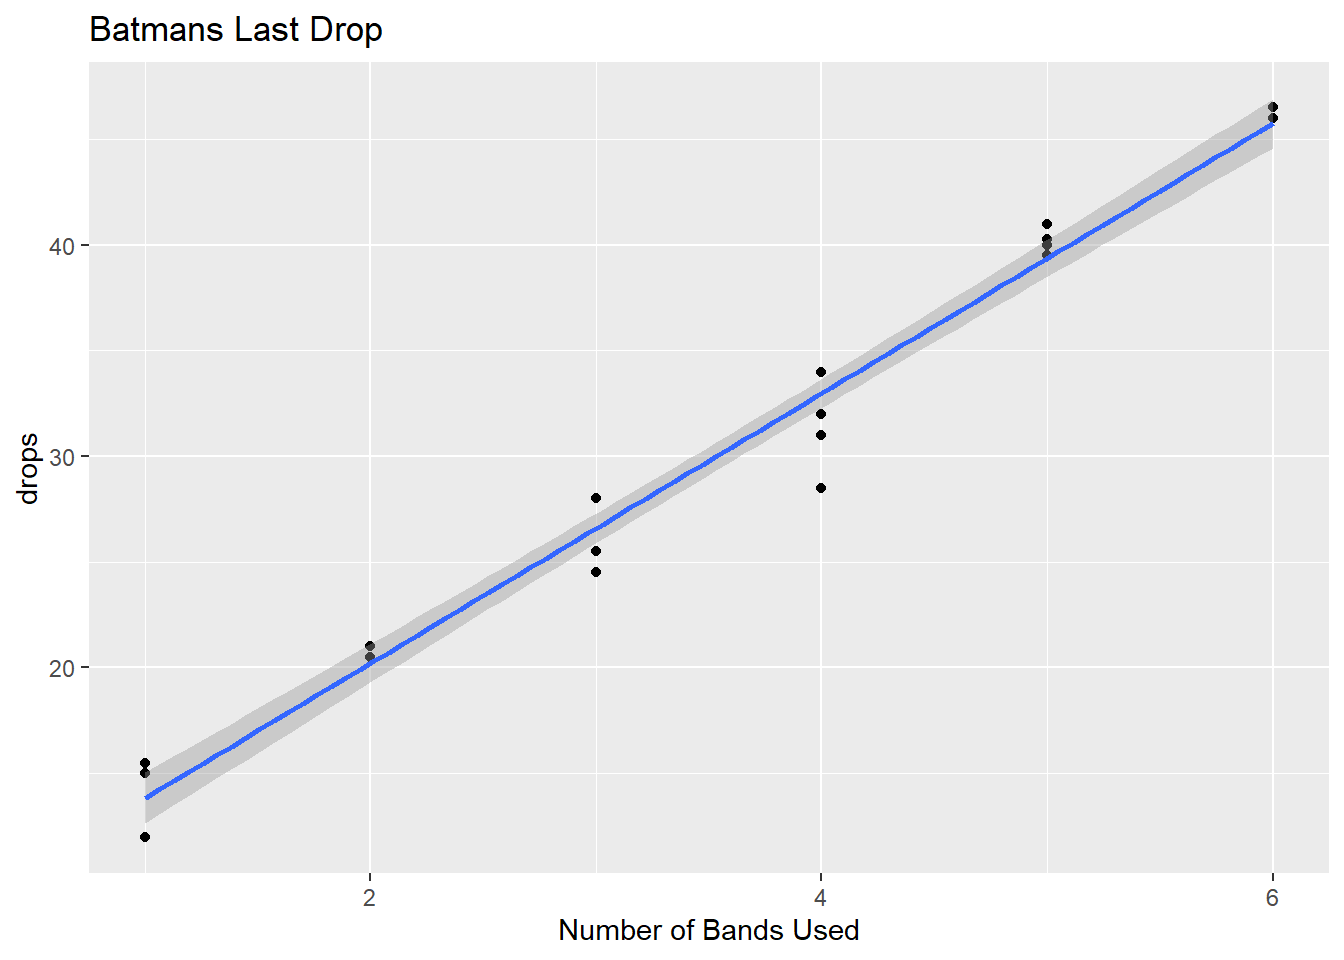
\includegraphics{Employee-Attrition_files/figure-latex/unnamed-chunk-5-1.pdf}

\begin{Shaded}
\begin{Highlighting}[]
\CommentTok{\# LONGEVITY | Department \#\#\#\#}
\NormalTok{attrition }\SpecialCharTok{\%\textgreater{}\%} \FunctionTok{ggplot}\NormalTok{(}\FunctionTok{aes}\NormalTok{(}\AttributeTok{x =}\NormalTok{ YearsAtCompany, }\AttributeTok{y =}\NormalTok{ Department, }\AttributeTok{color =}\NormalTok{ Attrition)) }\SpecialCharTok{+}
  \FunctionTok{geom\_boxplot}\NormalTok{() }\SpecialCharTok{+}
  \FunctionTok{geom\_vline}\NormalTok{(}\FunctionTok{aes}\NormalTok{(}\AttributeTok{xintercept =} \FunctionTok{mean}\NormalTok{(YearsAtCompany)), }\AttributeTok{color =} \StringTok{"black"}\NormalTok{, }\AttributeTok{linetype =} \StringTok{"dashed"}\NormalTok{) }\SpecialCharTok{+}
  \FunctionTok{ylab}\NormalTok{(}\StringTok{"Department"}\NormalTok{) }\SpecialCharTok{+}
  \FunctionTok{xlab}\NormalTok{(}\StringTok{"YearsAtCompany"}\NormalTok{) }\SpecialCharTok{+}
  \FunctionTok{scale\_color\_manual}\NormalTok{(}\AttributeTok{values =}\NormalTok{ colors)}
\end{Highlighting}
\end{Shaded}

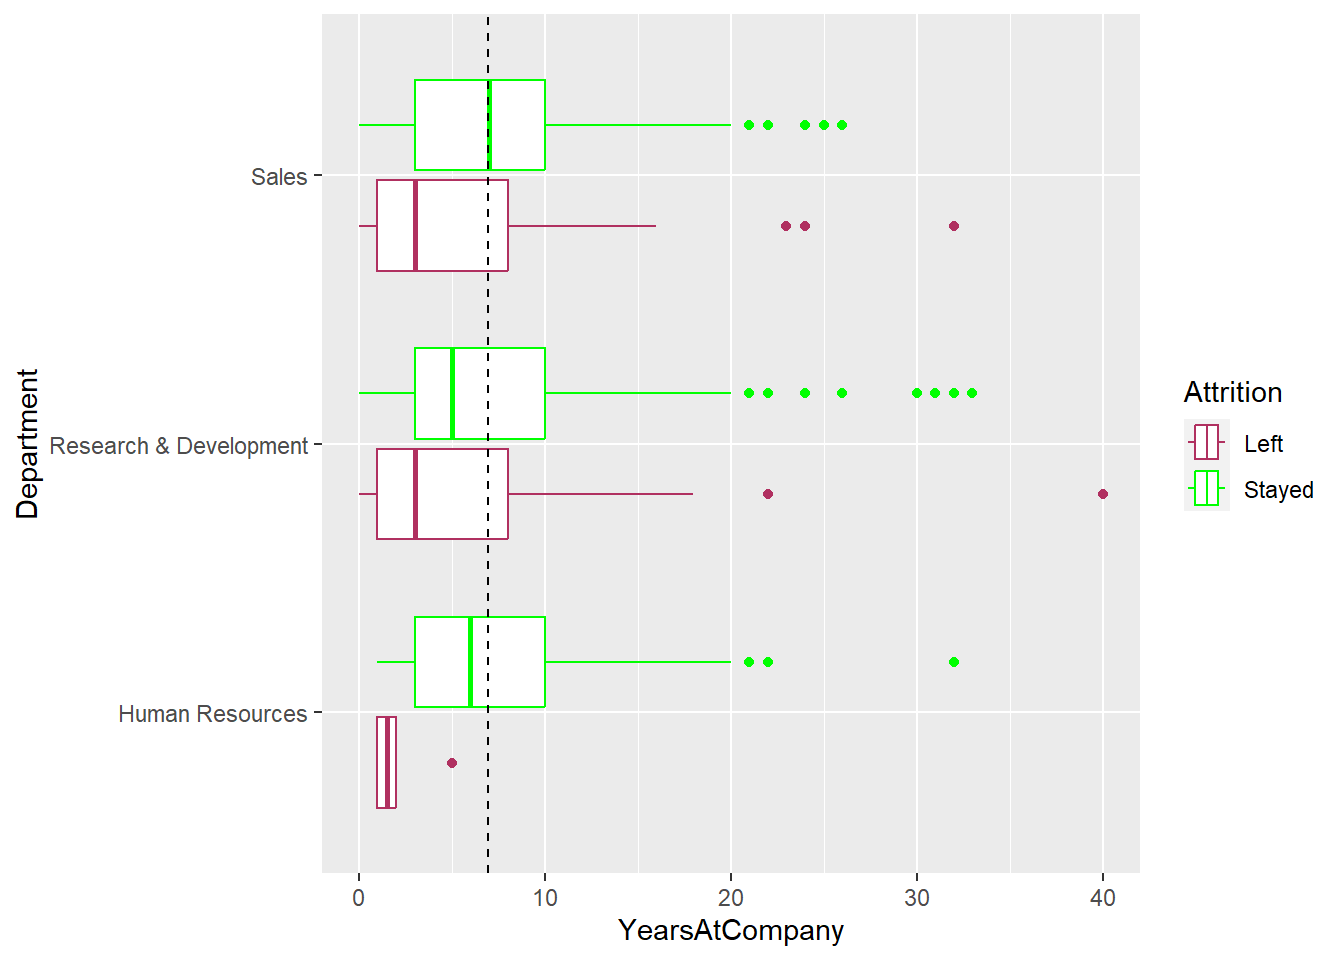
\includegraphics{Employee-Attrition_files/figure-latex/unnamed-chunk-6-1.pdf}

\begin{Shaded}
\begin{Highlighting}[]
\CommentTok{\# LONGEVITY | Department {-} Mean Line \#\#\#\# }
\NormalTok{attrition }\SpecialCharTok{\%\textgreater{}\%} \FunctionTok{ggplot}\NormalTok{(}\FunctionTok{aes}\NormalTok{(}\AttributeTok{x =}\NormalTok{ YearsAtCompany, }\AttributeTok{y =}\NormalTok{ Department, }\AttributeTok{color =}\NormalTok{ Attrition)) }\SpecialCharTok{+}
  \FunctionTok{geom\_point}\NormalTok{(}\AttributeTok{position =} \StringTok{"jitter"}\NormalTok{) }\SpecialCharTok{+}
  \FunctionTok{geom\_vline}\NormalTok{(}\FunctionTok{aes}\NormalTok{(}\AttributeTok{xintercept =} \FunctionTok{mean}\NormalTok{(YearsAtCompany)), }\AttributeTok{color =} \StringTok{"black"}\NormalTok{, }\AttributeTok{linetype =} \StringTok{"dashed"}\NormalTok{) }\SpecialCharTok{+}
  \CommentTok{\#annotate("text", x = mean(attrition$YearsAtCompany), y = max(attrition$Department), label = "Mean Line", vjust = {-}3) +}
  \FunctionTok{ylab}\NormalTok{(}\StringTok{"Department"}\NormalTok{) }\SpecialCharTok{+}
  \FunctionTok{xlab}\NormalTok{(}\StringTok{"YearsAtCompany"}\NormalTok{) }\SpecialCharTok{+}
  \FunctionTok{scale\_color\_manual}\NormalTok{(}\AttributeTok{values =}\NormalTok{ colors)}
\end{Highlighting}
\end{Shaded}

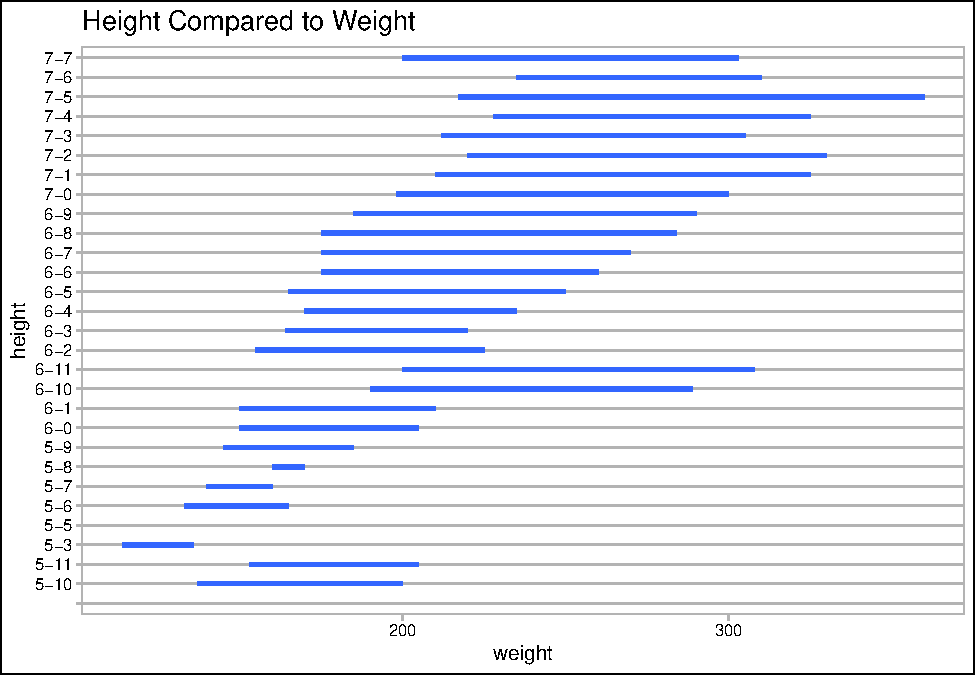
\includegraphics{Employee-Attrition_files/figure-latex/unnamed-chunk-7-1.pdf}

\begin{Shaded}
\begin{Highlighting}[]
\FunctionTok{summary}\NormalTok{(attrition}\SpecialCharTok{$}\NormalTok{YearsAtCompany)}
\end{Highlighting}
\end{Shaded}

\begin{verbatim}
##    Min. 1st Qu.  Median    Mean 3rd Qu.    Max. 
##   0.000   3.000   5.000   6.962  10.000  40.000
\end{verbatim}

\begin{Shaded}
\begin{Highlighting}[]
\CommentTok{\# LONGEVITY | Job Role \#\#\#\#}
\NormalTok{attrition }\SpecialCharTok{\%\textgreater{}\%} \FunctionTok{ggplot}\NormalTok{(}\FunctionTok{aes}\NormalTok{(}\AttributeTok{x =}\NormalTok{ YearsAtCompany, }\AttributeTok{y =}\NormalTok{ JobRole, }\AttributeTok{color =}\NormalTok{ Attrition)) }\SpecialCharTok{+}
  \FunctionTok{geom\_point}\NormalTok{(}\AttributeTok{position =} \StringTok{"jitter"}\NormalTok{) }\SpecialCharTok{+}
  \FunctionTok{ylab}\NormalTok{(}\StringTok{"JobRole"}\NormalTok{) }\SpecialCharTok{+}
  \FunctionTok{xlab}\NormalTok{(}\StringTok{"YearsAtCompany"}\NormalTok{) }\SpecialCharTok{+}
  \FunctionTok{scale\_color\_manual}\NormalTok{(}\AttributeTok{values =}\NormalTok{ colors)}
\end{Highlighting}
\end{Shaded}

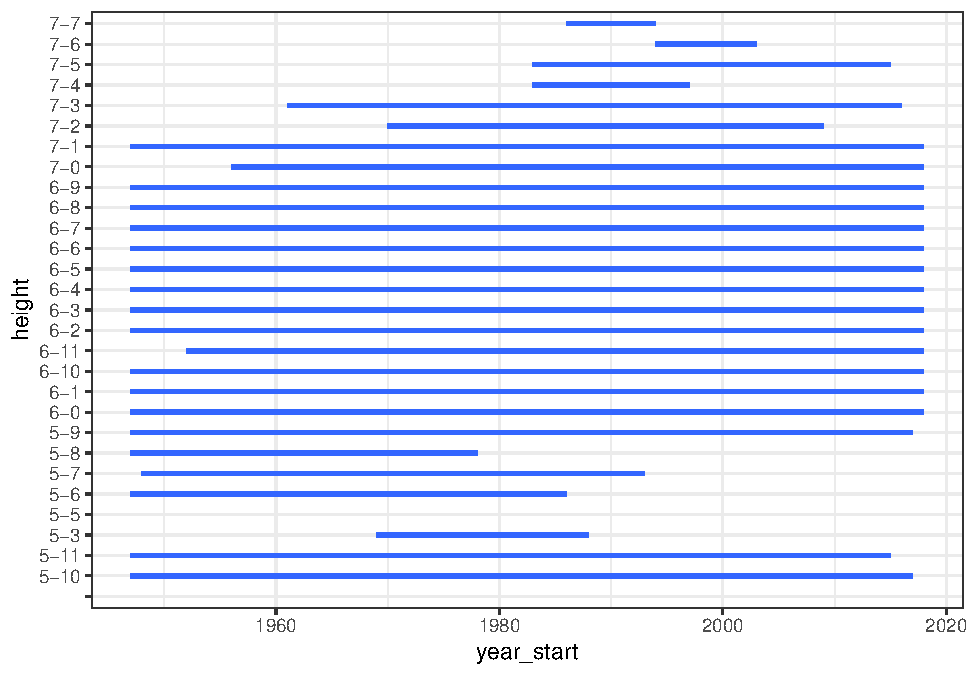
\includegraphics{Employee-Attrition_files/figure-latex/unnamed-chunk-9-1.pdf}

\begin{Shaded}
\begin{Highlighting}[]
\CommentTok{\# LONGEVITY | Job Role {-} Mean Line \#\#\#\# }
\NormalTok{attrition }\SpecialCharTok{\%\textgreater{}\%} \FunctionTok{ggplot}\NormalTok{(}\FunctionTok{aes}\NormalTok{(}\AttributeTok{x =}\NormalTok{ YearsAtCompany, }\AttributeTok{y =}\NormalTok{ JobRole, }\AttributeTok{color =}\NormalTok{ Attrition)) }\SpecialCharTok{+}
  \FunctionTok{geom\_boxplot}\NormalTok{() }\SpecialCharTok{+}
  \FunctionTok{geom\_vline}\NormalTok{(}\FunctionTok{aes}\NormalTok{(}\AttributeTok{xintercept =} \FunctionTok{mean}\NormalTok{(YearsAtCompany)), }\AttributeTok{color =} \StringTok{"black"}\NormalTok{, }\AttributeTok{linetype =} \StringTok{"dashed"}\NormalTok{) }\SpecialCharTok{+}
  \CommentTok{\#annotate("text", x = mean(attrition$YearsAtCompany), y = max(attrition$JobRole), label = "Mean Line", vjust = 0) +}
  \FunctionTok{ylab}\NormalTok{(}\StringTok{"JobRole"}\NormalTok{) }\SpecialCharTok{+}
  \FunctionTok{xlab}\NormalTok{(}\StringTok{"YearsAtCompany"}\NormalTok{) }\SpecialCharTok{+}
  \FunctionTok{scale\_color\_manual}\NormalTok{(}\AttributeTok{values =}\NormalTok{ colors)}
\end{Highlighting}
\end{Shaded}

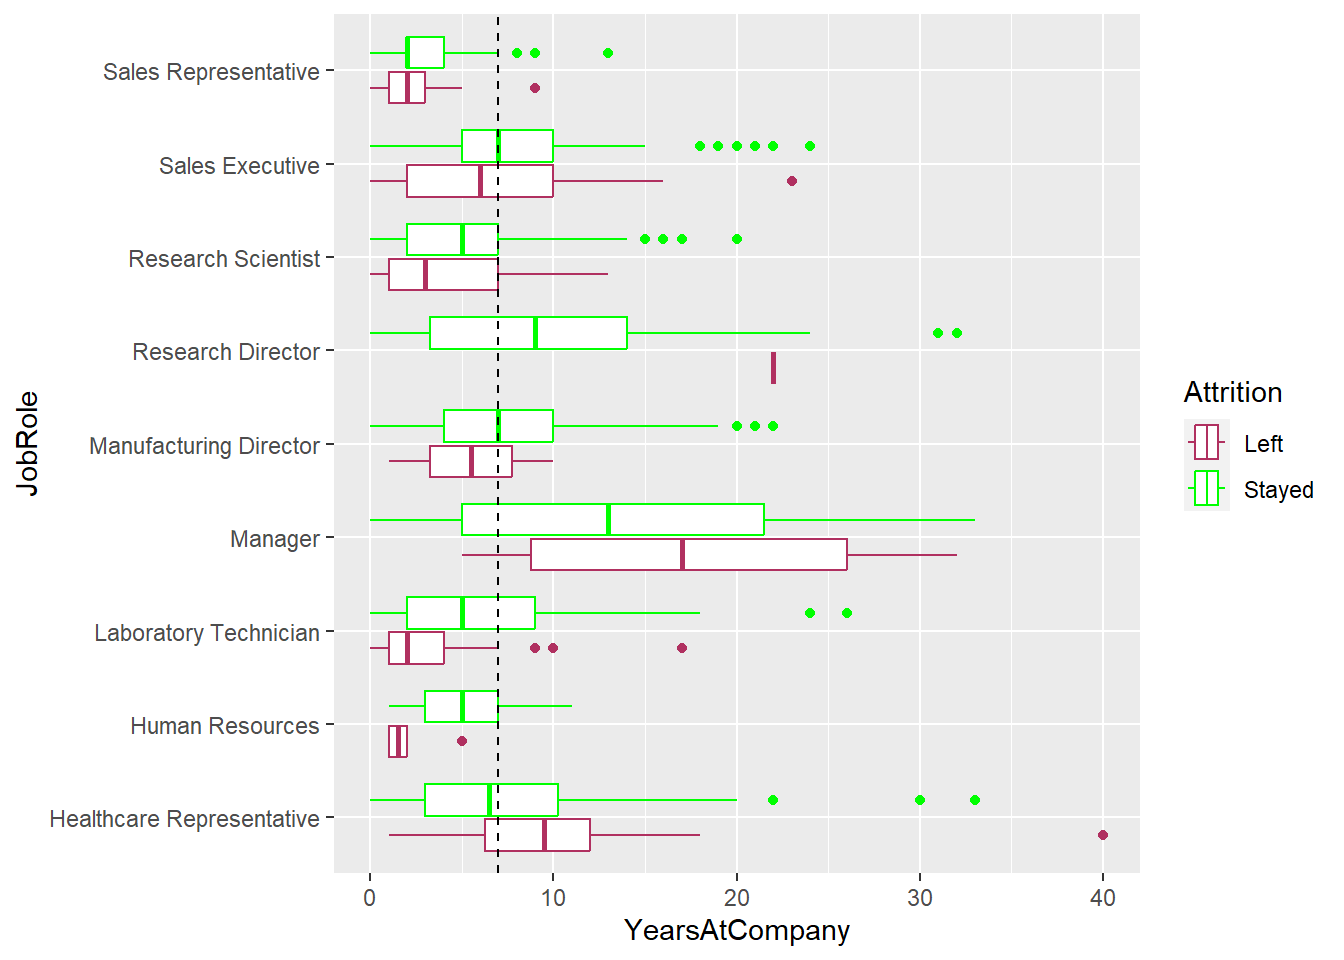
\includegraphics{Employee-Attrition_files/figure-latex/unnamed-chunk-10-1.pdf}

\hypertarget{job-roles-matter}{%
\subsection{Job Roles Matter}\label{job-roles-matter}}

At this point I am noticing that Job Roles play a part in the Attrition
Process. The next few chart wil investigate this theory

\begin{Shaded}
\begin{Highlighting}[]
\CommentTok{\# AGE | Department \#\#\#\#}
\NormalTok{attrition }\SpecialCharTok{\%\textgreater{}\%} \FunctionTok{ggplot}\NormalTok{(}\FunctionTok{aes}\NormalTok{(}\AttributeTok{x =}\NormalTok{ Age, }\AttributeTok{y =}\NormalTok{ Department, }\AttributeTok{color =}\NormalTok{ Attrition)) }\SpecialCharTok{+}
  \FunctionTok{geom\_point}\NormalTok{(}\AttributeTok{position =} \StringTok{"jitter"}\NormalTok{) }\SpecialCharTok{+}
  \FunctionTok{ylab}\NormalTok{(}\StringTok{"Department"}\NormalTok{) }\SpecialCharTok{+}
  \FunctionTok{xlab}\NormalTok{(}\StringTok{"Age"}\NormalTok{) }\SpecialCharTok{+}
  \FunctionTok{scale\_color\_manual}\NormalTok{(}\AttributeTok{values =}\NormalTok{ colors)}
\end{Highlighting}
\end{Shaded}

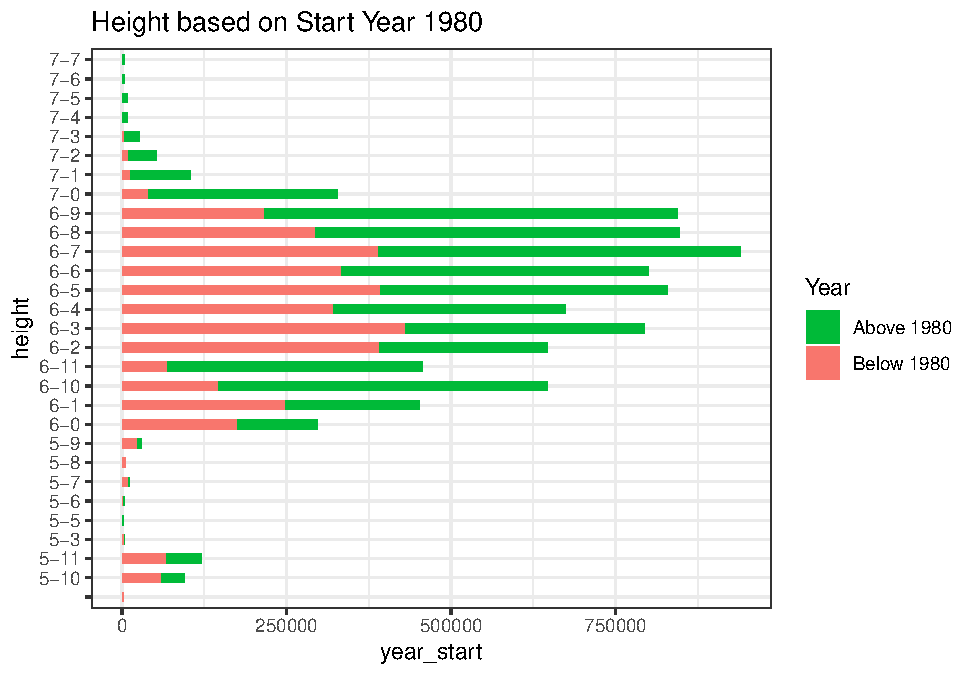
\includegraphics{Employee-Attrition_files/figure-latex/unnamed-chunk-11-1.pdf}

\begin{Shaded}
\begin{Highlighting}[]
\CommentTok{\# AGE  | Department  {-} MEAN \#\#\#\#}
\NormalTok{attrition }\SpecialCharTok{\%\textgreater{}\%} \FunctionTok{ggplot}\NormalTok{(}\FunctionTok{aes}\NormalTok{(}\AttributeTok{x =}\NormalTok{ Age, }\AttributeTok{y =}\NormalTok{ Department, }\AttributeTok{color =}\NormalTok{ Attrition)) }\SpecialCharTok{+}
  \FunctionTok{geom\_point}\NormalTok{(}\AttributeTok{position =} \StringTok{"jitter"}\NormalTok{) }\SpecialCharTok{+}
  \FunctionTok{geom\_vline}\NormalTok{(}\FunctionTok{aes}\NormalTok{(}\AttributeTok{xintercept =} \FunctionTok{mean}\NormalTok{(Age)), }\AttributeTok{color =} \StringTok{"black"}\NormalTok{, }\AttributeTok{linetype =} \StringTok{"dashed"}\NormalTok{) }\SpecialCharTok{+}
  \CommentTok{\#annotate("text", x = mean(attrition$Age), y = max(attrition$Department), label = "Mean Line", vjust = {-}3) +}
  \FunctionTok{ylab}\NormalTok{(}\StringTok{"Department"}\NormalTok{) }\SpecialCharTok{+}
  \FunctionTok{xlab}\NormalTok{(}\StringTok{"Age"}\NormalTok{) }\SpecialCharTok{+}
  \FunctionTok{scale\_color\_manual}\NormalTok{(}\AttributeTok{values =}\NormalTok{ colors)}
\end{Highlighting}
\end{Shaded}

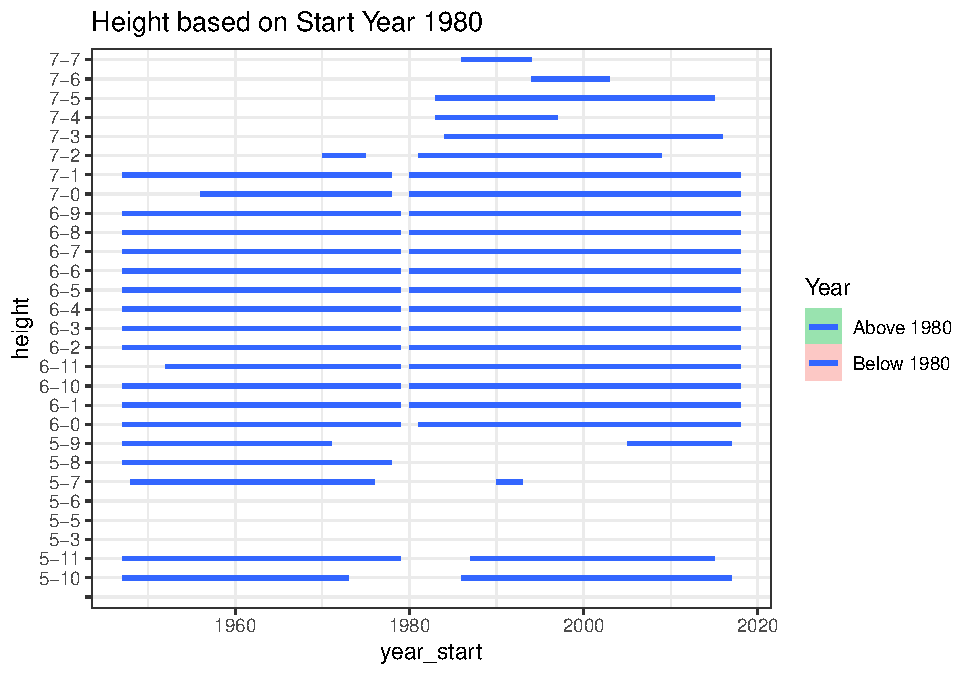
\includegraphics{Employee-Attrition_files/figure-latex/unnamed-chunk-12-1.pdf}

\begin{Shaded}
\begin{Highlighting}[]
\CommentTok{\# AGE {-} JobRole \#\#\#\#}
\NormalTok{attrition }\SpecialCharTok{\%\textgreater{}\%} \FunctionTok{ggplot}\NormalTok{(}\FunctionTok{aes}\NormalTok{(}\AttributeTok{x =}\NormalTok{ Age, }\AttributeTok{y =}\NormalTok{ JobRole, }\AttributeTok{color =}\NormalTok{ Attrition)) }\SpecialCharTok{+}
  \FunctionTok{geom\_point}\NormalTok{(}\AttributeTok{position =} \StringTok{"jitter"}\NormalTok{) }\SpecialCharTok{+}
  \FunctionTok{ylab}\NormalTok{(}\StringTok{"JobRole"}\NormalTok{) }\SpecialCharTok{+}
  \FunctionTok{xlab}\NormalTok{(}\StringTok{"Age"}\NormalTok{) }\SpecialCharTok{+}
  \FunctionTok{scale\_color\_manual}\NormalTok{(}\AttributeTok{values =}\NormalTok{ colors)}
\end{Highlighting}
\end{Shaded}

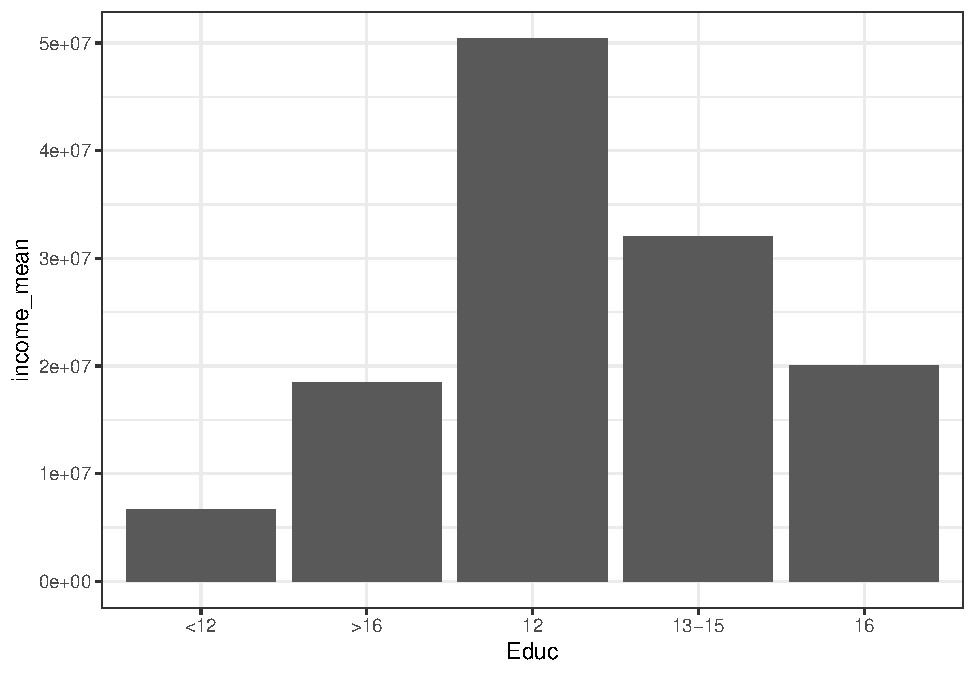
\includegraphics{Employee-Attrition_files/figure-latex/unnamed-chunk-13-1.pdf}

\begin{Shaded}
\begin{Highlighting}[]
\CommentTok{\# AGE | JobRole {-} MEAN \#\#\#\#}
\NormalTok{attrition }\SpecialCharTok{\%\textgreater{}\%} \FunctionTok{ggplot}\NormalTok{(}\FunctionTok{aes}\NormalTok{(}\AttributeTok{x =}\NormalTok{ Age, }\AttributeTok{y =}\NormalTok{ JobRole, }\AttributeTok{color =}\NormalTok{ Attrition)) }\SpecialCharTok{+}
  \FunctionTok{geom\_boxplot}\NormalTok{() }\SpecialCharTok{+}
  \FunctionTok{geom\_vline}\NormalTok{(}\FunctionTok{aes}\NormalTok{(}\AttributeTok{xintercept =} \FunctionTok{mean}\NormalTok{(Age)), }\AttributeTok{color =} \StringTok{"black"}\NormalTok{, }\AttributeTok{linetype =} \StringTok{"dashed"}\NormalTok{) }\SpecialCharTok{+}
  \CommentTok{\#annotate("text", x = mean(attrition$Age), y = max(attrition$JobRole), label = "Mean Line", vjust = {-}3) +}
  \FunctionTok{ylab}\NormalTok{(}\StringTok{"JobRole"}\NormalTok{) }\SpecialCharTok{+}
  \FunctionTok{xlab}\NormalTok{(}\StringTok{"Age"}\NormalTok{) }\SpecialCharTok{+}
  \FunctionTok{scale\_color\_manual}\NormalTok{(}\AttributeTok{values =}\NormalTok{ colors)}
\end{Highlighting}
\end{Shaded}

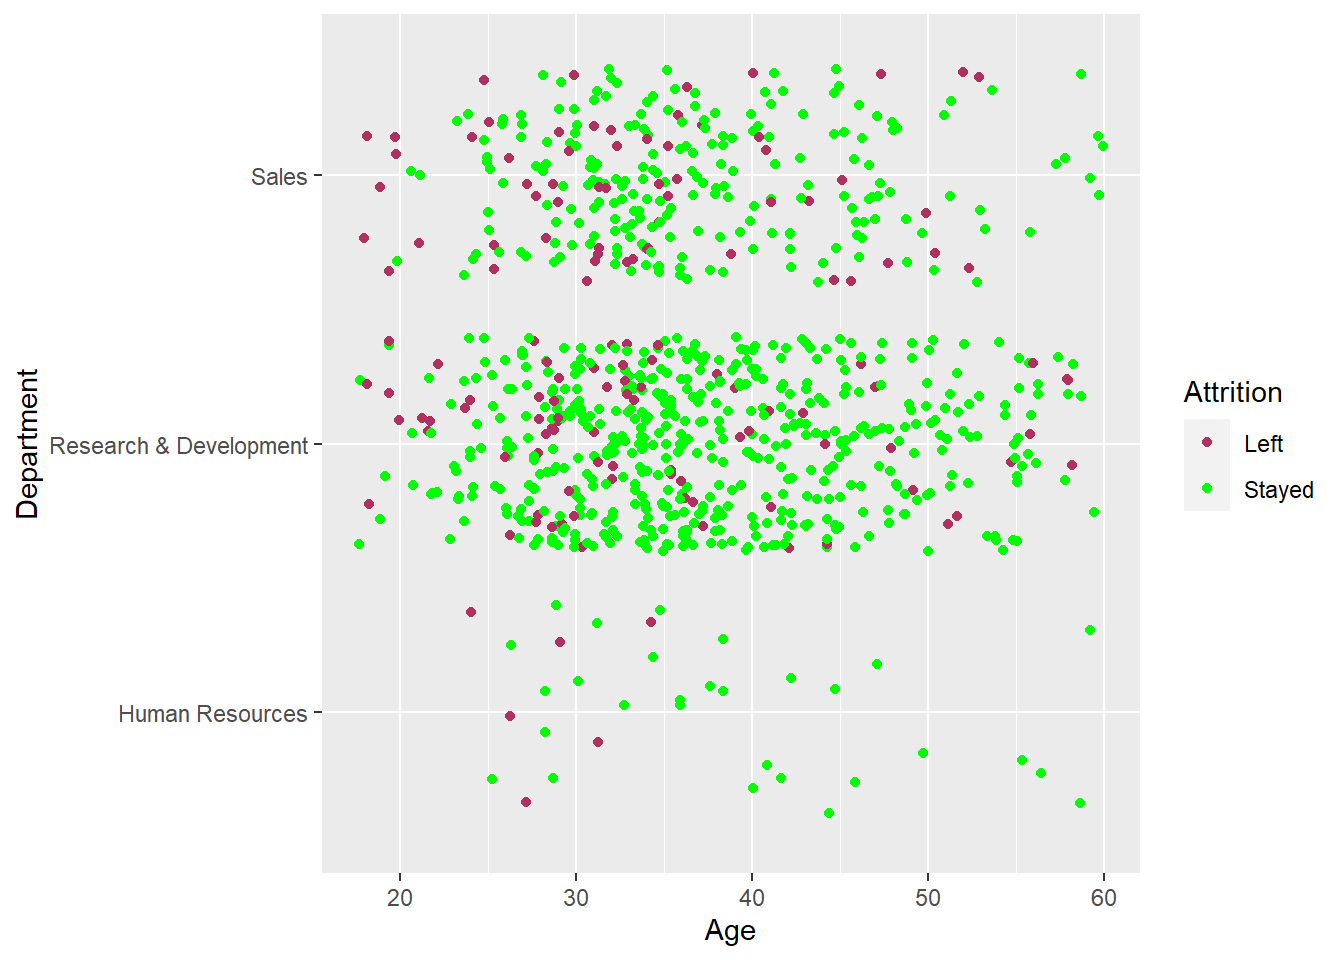
\includegraphics{Employee-Attrition_files/figure-latex/unnamed-chunk-14-1.pdf}

\begin{Shaded}
\begin{Highlighting}[]
\FunctionTok{summary}\NormalTok{(attrition}\SpecialCharTok{$}\NormalTok{Age)}
\end{Highlighting}
\end{Shaded}

\begin{verbatim}
##    Min. 1st Qu.  Median    Mean 3rd Qu.    Max. 
##   18.00   30.00   35.00   36.83   43.00   60.00
\end{verbatim}

\begin{Shaded}
\begin{Highlighting}[]
\CommentTok{\# Younger Job Roles \#\#\#\#}
\NormalTok{y }\OtherTok{\textless{}{-}} \FunctionTok{filter}\NormalTok{(attrition, JobRole }\SpecialCharTok{==} \StringTok{"Sales Representative"} \SpecialCharTok{|}\NormalTok{ JobRole }\SpecialCharTok{==} \StringTok{"Human Resources"}\NormalTok{) }\SpecialCharTok{\%\textgreater{}\%}
  \FunctionTok{ggplot}\NormalTok{(}\FunctionTok{aes}\NormalTok{(}\AttributeTok{x =}\NormalTok{ Age, }\AttributeTok{y =}\NormalTok{ JobRole, }\AttributeTok{color =}\NormalTok{ Attrition)) }\SpecialCharTok{+}
  \FunctionTok{geom\_point}\NormalTok{(}\AttributeTok{position =} \StringTok{"jitter"}\NormalTok{) }\SpecialCharTok{+}
  \FunctionTok{geom\_vline}\NormalTok{(}\FunctionTok{aes}\NormalTok{(}\AttributeTok{xintercept =} \FunctionTok{mean}\NormalTok{(Age)), }\AttributeTok{color =} \StringTok{"black"}\NormalTok{, }\AttributeTok{linetype =} \StringTok{"dashed"}\NormalTok{) }\SpecialCharTok{+}
  \FunctionTok{ylab}\NormalTok{(}\StringTok{"JobRole"}\NormalTok{) }\SpecialCharTok{+}
  \FunctionTok{xlab}\NormalTok{(}\StringTok{"Age"}\NormalTok{) }\SpecialCharTok{+}
  \FunctionTok{scale\_color\_manual}\NormalTok{(}\AttributeTok{values =}\NormalTok{ colors) }\SpecialCharTok{+}
  \FunctionTok{ggtitle}\NormalTok{(}\StringTok{"Younger Ages"}\NormalTok{) }\SpecialCharTok{+}
  \FunctionTok{theme}\NormalTok{(}\AttributeTok{legend.position =} \StringTok{"none"}\NormalTok{) }\SpecialCharTok{+}
  \FunctionTok{theme}\NormalTok{(}\AttributeTok{plot.title =} \FunctionTok{element\_text}\NormalTok{(}\AttributeTok{hjust =} \FloatTok{0.5}\NormalTok{)) }
  

\CommentTok{\# OLDER Job Roles \#\#\#\#}
\NormalTok{o }\OtherTok{\textless{}{-}} \FunctionTok{filter}\NormalTok{(attrition, JobRole }\SpecialCharTok{==} \StringTok{"Manager"} \SpecialCharTok{|}\NormalTok{ JobRole }\SpecialCharTok{==} \StringTok{"Research Director"}\NormalTok{ ) }\SpecialCharTok{\%\textgreater{}\%}
  \FunctionTok{ggplot}\NormalTok{(}\FunctionTok{aes}\NormalTok{(}\AttributeTok{x =}\NormalTok{ Age, }\AttributeTok{y =}\NormalTok{ JobRole, }\AttributeTok{color =}\NormalTok{ Attrition)) }\SpecialCharTok{+}
  \FunctionTok{geom\_point}\NormalTok{(}\AttributeTok{position =} \StringTok{"jitter"}\NormalTok{) }\SpecialCharTok{+}
  \FunctionTok{geom\_vline}\NormalTok{(}\FunctionTok{aes}\NormalTok{(}\AttributeTok{xintercept =} \FunctionTok{mean}\NormalTok{(Age)), }\AttributeTok{color =} \StringTok{"black"}\NormalTok{, }\AttributeTok{linetype =} \StringTok{"dashed"}\NormalTok{) }\SpecialCharTok{+}
  \FunctionTok{ylab}\NormalTok{(}\StringTok{"JobRole"}\NormalTok{) }\SpecialCharTok{+}
  \FunctionTok{xlab}\NormalTok{(}\StringTok{"Age"}\NormalTok{) }\SpecialCharTok{+}
  \FunctionTok{scale\_color\_manual}\NormalTok{(}\AttributeTok{values =}\NormalTok{ colors) }\SpecialCharTok{+}
  \FunctionTok{ggtitle}\NormalTok{(}\StringTok{"Older Ages"}\NormalTok{) }\SpecialCharTok{+}
  \FunctionTok{theme}\NormalTok{(}\AttributeTok{legend.position =} \StringTok{"none"}\NormalTok{) }\SpecialCharTok{+}
  \FunctionTok{theme}\NormalTok{(}\AttributeTok{plot.title =} \FunctionTok{element\_text}\NormalTok{(}\AttributeTok{hjust =} \FloatTok{0.5}\NormalTok{)) }


\CommentTok{\# ALL AGES Job Roles \#\#\#\#}
\NormalTok{a }\OtherTok{\textless{}{-}} \FunctionTok{filter}\NormalTok{(attrition, JobRole }\SpecialCharTok{==} \StringTok{"Research Scientist"} \SpecialCharTok{|}\NormalTok{ JobRole }\SpecialCharTok{==} \StringTok{"Sales Executive"}  \SpecialCharTok{|}\NormalTok{ JobRole }\SpecialCharTok{==} \StringTok{"Laboratory Technician"} \SpecialCharTok{|}\NormalTok{ JobRole }\SpecialCharTok{==} \StringTok{"Healthcare Representative"}\SpecialCharTok{|}\NormalTok{ JobRole }\SpecialCharTok{==} \StringTok{"Manufacturing Director"}\NormalTok{ ) }\SpecialCharTok{\%\textgreater{}\%}
  \FunctionTok{ggplot}\NormalTok{(}\FunctionTok{aes}\NormalTok{(}\AttributeTok{x =}\NormalTok{ Age, }\AttributeTok{y =}\NormalTok{ JobRole, }\AttributeTok{color =}\NormalTok{ Attrition)) }\SpecialCharTok{+}
  \FunctionTok{geom\_point}\NormalTok{(}\AttributeTok{position =} \StringTok{"jitter"}\NormalTok{) }\SpecialCharTok{+}
  \FunctionTok{geom\_vline}\NormalTok{(}\FunctionTok{aes}\NormalTok{(}\AttributeTok{xintercept =} \FunctionTok{mean}\NormalTok{(Age)), }\AttributeTok{color =} \StringTok{"black"}\NormalTok{, }\AttributeTok{linetype =} \StringTok{"dashed"}\NormalTok{) }\SpecialCharTok{+}
  \FunctionTok{ylab}\NormalTok{(}\StringTok{"JobRole"}\NormalTok{) }\SpecialCharTok{+}
  \FunctionTok{xlab}\NormalTok{(}\StringTok{"Age"}\NormalTok{) }\SpecialCharTok{+}
  \FunctionTok{scale\_color\_manual}\NormalTok{(}\AttributeTok{values =}\NormalTok{ colors) }\SpecialCharTok{+}
  \FunctionTok{ggtitle}\NormalTok{(}\StringTok{"All Ages"}\NormalTok{) }\SpecialCharTok{+}
  \FunctionTok{theme}\NormalTok{(}\AttributeTok{legend.position =} \StringTok{"none"}\NormalTok{) }\SpecialCharTok{+}
  \FunctionTok{theme}\NormalTok{(}\AttributeTok{plot.title =} \FunctionTok{element\_text}\NormalTok{(}\AttributeTok{hjust =} \FloatTok{0.5}\NormalTok{)) }

\FunctionTok{grid.arrange}\NormalTok{(y, o, a, }\AttributeTok{nrow =} \DecValTok{3}\NormalTok{)}
\end{Highlighting}
\end{Shaded}

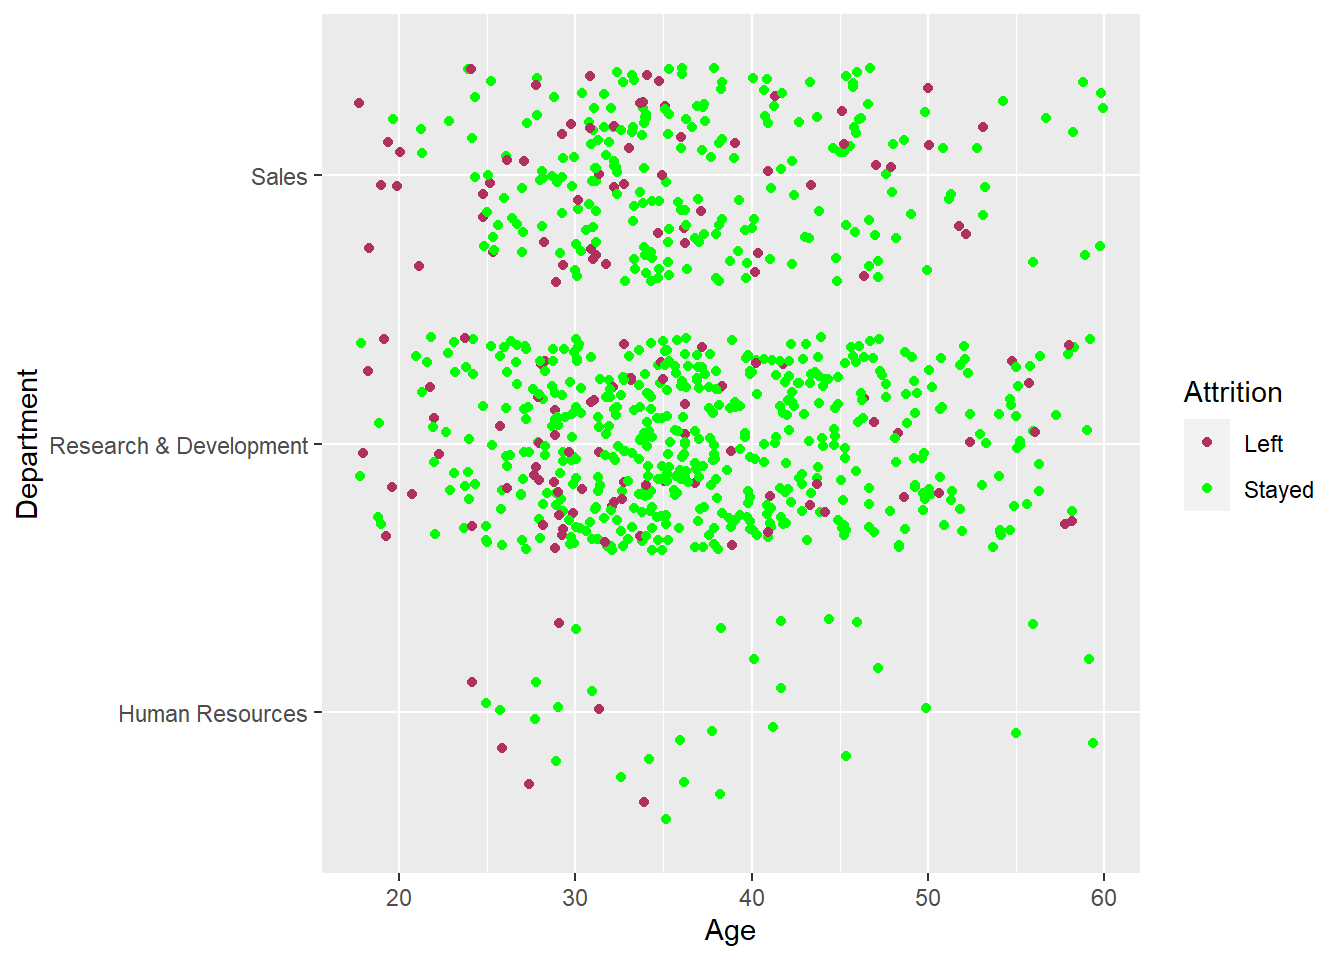
\includegraphics{Employee-Attrition_files/figure-latex/unnamed-chunk-16-1.pdf}

\hypertarget{work-life-balance-review}{%
\subsection{Work Life Balance Review}\label{work-life-balance-review}}

\begin{Shaded}
\begin{Highlighting}[]
\CommentTok{\# Younger Job Roles \#\#\#\#}
\NormalTok{y }\OtherTok{\textless{}{-}} \FunctionTok{filter}\NormalTok{(attrition, JobRole }\SpecialCharTok{==} \StringTok{"Sales Representative"} \SpecialCharTok{|}\NormalTok{ JobRole }\SpecialCharTok{==} \StringTok{"Human Resources"}\NormalTok{) }\SpecialCharTok{\%\textgreater{}\%}
  \FunctionTok{ggplot}\NormalTok{(}\FunctionTok{aes}\NormalTok{(}\AttributeTok{x =}\NormalTok{ WorkLifeBalance, }\AttributeTok{y =}\NormalTok{ JobRole, }\AttributeTok{color =}\NormalTok{ Attrition)) }\SpecialCharTok{+}
  \FunctionTok{geom\_point}\NormalTok{(}\AttributeTok{position =} \StringTok{"jitter"}\NormalTok{) }\SpecialCharTok{+}
  \FunctionTok{ylab}\NormalTok{(}\StringTok{"JobRole"}\NormalTok{) }\SpecialCharTok{+}
  \FunctionTok{xlab}\NormalTok{(}\StringTok{"WorkLifeBalance"}\NormalTok{) }\SpecialCharTok{+}
  \FunctionTok{scale\_color\_manual}\NormalTok{(}\AttributeTok{values =}\NormalTok{ colors) }\SpecialCharTok{+}
  \FunctionTok{ggtitle}\NormalTok{(}\StringTok{"Younger Ages"}\NormalTok{) }\SpecialCharTok{+}
  \FunctionTok{theme}\NormalTok{(}\AttributeTok{legend.position =} \StringTok{"none"}\NormalTok{) }\SpecialCharTok{+}
  \FunctionTok{theme}\NormalTok{(}\AttributeTok{plot.title =} \FunctionTok{element\_text}\NormalTok{(}\AttributeTok{hjust =} \FloatTok{0.5}\NormalTok{)) }
  

\CommentTok{\# OLDER Job Roles \#\#\#\#}
\NormalTok{o }\OtherTok{\textless{}{-}} \FunctionTok{filter}\NormalTok{(attrition, JobRole }\SpecialCharTok{==} \StringTok{"Manager"} \SpecialCharTok{|}\NormalTok{ JobRole }\SpecialCharTok{==} \StringTok{"Research Director"}\NormalTok{ ) }\SpecialCharTok{\%\textgreater{}\%}
  \FunctionTok{ggplot}\NormalTok{(}\FunctionTok{aes}\NormalTok{(}\AttributeTok{x =}\NormalTok{ WorkLifeBalance, }\AttributeTok{y =}\NormalTok{ JobRole, }\AttributeTok{color =}\NormalTok{ Attrition)) }\SpecialCharTok{+}
  \FunctionTok{geom\_point}\NormalTok{(}\AttributeTok{position =} \StringTok{"jitter"}\NormalTok{) }\SpecialCharTok{+}
  \FunctionTok{ylab}\NormalTok{(}\StringTok{"JobRole"}\NormalTok{) }\SpecialCharTok{+}
  \FunctionTok{xlab}\NormalTok{(}\StringTok{"WorkLifeBalance"}\NormalTok{) }\SpecialCharTok{+}
  \FunctionTok{scale\_color\_manual}\NormalTok{(}\AttributeTok{values =}\NormalTok{ colors) }\SpecialCharTok{+}
  \FunctionTok{ggtitle}\NormalTok{(}\StringTok{"Older Ages"}\NormalTok{) }\SpecialCharTok{+}
  \FunctionTok{theme}\NormalTok{(}\AttributeTok{legend.position =} \StringTok{"none"}\NormalTok{) }\SpecialCharTok{+}
  \FunctionTok{theme}\NormalTok{(}\AttributeTok{plot.title =} \FunctionTok{element\_text}\NormalTok{(}\AttributeTok{hjust =} \FloatTok{0.5}\NormalTok{)) }


\CommentTok{\# ALL AGES Job Roles \#\#\#\#}
\NormalTok{a }\OtherTok{\textless{}{-}} \FunctionTok{filter}\NormalTok{(attrition, JobRole }\SpecialCharTok{==} \StringTok{"Research Scientist"} \SpecialCharTok{|}\NormalTok{ JobRole }\SpecialCharTok{==} \StringTok{"Sales Executive"}  \SpecialCharTok{|}\NormalTok{ JobRole }\SpecialCharTok{==} \StringTok{"Laboratory Technician"} \SpecialCharTok{|}\NormalTok{ JobRole }\SpecialCharTok{==} \StringTok{"Healthcare Representative"}\SpecialCharTok{|}\NormalTok{ JobRole }\SpecialCharTok{==} \StringTok{"Manufacturing Director"}\NormalTok{ ) }\SpecialCharTok{\%\textgreater{}\%}
  \FunctionTok{ggplot}\NormalTok{(}\FunctionTok{aes}\NormalTok{(}\AttributeTok{x =}\NormalTok{ WorkLifeBalance, }\AttributeTok{y =}\NormalTok{ JobRole, }\AttributeTok{color =}\NormalTok{ Attrition)) }\SpecialCharTok{+}
  \FunctionTok{geom\_point}\NormalTok{(}\AttributeTok{position =} \StringTok{"jitter"}\NormalTok{) }\SpecialCharTok{+}
  \FunctionTok{ylab}\NormalTok{(}\StringTok{"JobRole"}\NormalTok{) }\SpecialCharTok{+}
  \FunctionTok{xlab}\NormalTok{(}\StringTok{"WorkLifeBalance"}\NormalTok{) }\SpecialCharTok{+}
  \FunctionTok{scale\_color\_manual}\NormalTok{(}\AttributeTok{values =}\NormalTok{ colors) }\SpecialCharTok{+}
  \FunctionTok{ggtitle}\NormalTok{(}\StringTok{"All Ages"}\NormalTok{) }\SpecialCharTok{+}
  \FunctionTok{theme}\NormalTok{(}\AttributeTok{legend.position =} \StringTok{"none"}\NormalTok{) }\SpecialCharTok{+}
  \FunctionTok{theme}\NormalTok{(}\AttributeTok{plot.title =} \FunctionTok{element\_text}\NormalTok{(}\AttributeTok{hjust =} \FloatTok{0.5}\NormalTok{)) }

\FunctionTok{grid.arrange}\NormalTok{(y, o, a, }\AttributeTok{nrow =} \DecValTok{3}\NormalTok{)}
\end{Highlighting}
\end{Shaded}

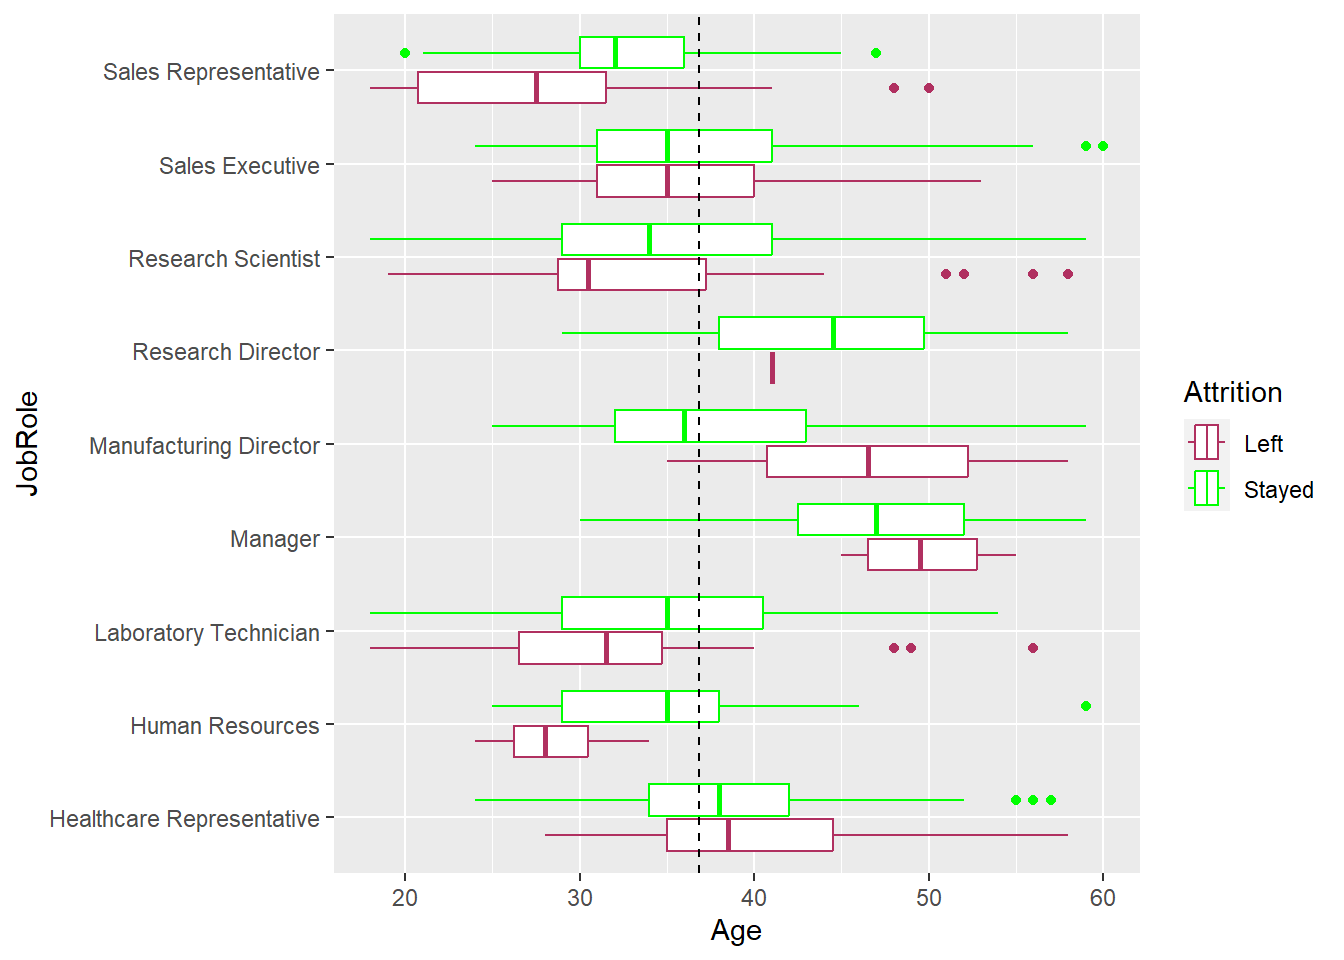
\includegraphics{Employee-Attrition_files/figure-latex/unnamed-chunk-17-1.pdf}

\hypertarget{money-importance-review}{%
\subsection{Money Importance Review}\label{money-importance-review}}

\begin{Shaded}
\begin{Highlighting}[]
\CommentTok{\# Younger Job Roles \#\#\#\#}
\NormalTok{y }\OtherTok{\textless{}{-}} \FunctionTok{filter}\NormalTok{(attrition, JobRole }\SpecialCharTok{==} \StringTok{"Sales Representative"} \SpecialCharTok{|}\NormalTok{ JobRole }\SpecialCharTok{==} \StringTok{"Human Resources"}\NormalTok{) }\SpecialCharTok{\%\textgreater{}\%}
  \FunctionTok{ggplot}\NormalTok{(}\FunctionTok{aes}\NormalTok{(}\AttributeTok{x =}\NormalTok{ MonthlyIncome, }\AttributeTok{y =}\NormalTok{ JobRole, }\AttributeTok{color =}\NormalTok{ Attrition)) }\SpecialCharTok{+}
  \FunctionTok{geom\_boxplot}\NormalTok{() }\SpecialCharTok{+}
  \FunctionTok{geom\_vline}\NormalTok{(}\FunctionTok{aes}\NormalTok{(}\AttributeTok{xintercept =} \FunctionTok{mean}\NormalTok{(MonthlyIncome)), }\AttributeTok{color =} \StringTok{"black"}\NormalTok{, }\AttributeTok{linetype =} \StringTok{"dashed"}\NormalTok{) }\SpecialCharTok{+}
  \FunctionTok{ylab}\NormalTok{(}\StringTok{"JobRole"}\NormalTok{) }\SpecialCharTok{+}
  \FunctionTok{xlab}\NormalTok{(}\StringTok{"MonthlyIncome"}\NormalTok{) }\SpecialCharTok{+}
  \FunctionTok{scale\_color\_manual}\NormalTok{(}\AttributeTok{values =}\NormalTok{ colors) }\SpecialCharTok{+}
  \FunctionTok{ggtitle}\NormalTok{(}\StringTok{"Younger Ages"}\NormalTok{) }\SpecialCharTok{+}
  \FunctionTok{theme}\NormalTok{(}\AttributeTok{legend.position =} \StringTok{"none"}\NormalTok{) }\SpecialCharTok{+}
  \FunctionTok{theme}\NormalTok{(}\AttributeTok{plot.title =} \FunctionTok{element\_text}\NormalTok{(}\AttributeTok{hjust =} \FloatTok{0.5}\NormalTok{)) }
  

\CommentTok{\# OLDER Job Roles \#\#\#\#}
\NormalTok{o }\OtherTok{\textless{}{-}} \FunctionTok{filter}\NormalTok{(attrition, JobRole }\SpecialCharTok{==} \StringTok{"Manager"} \SpecialCharTok{|}\NormalTok{ JobRole }\SpecialCharTok{==} \StringTok{"Research Director"}\NormalTok{ ) }\SpecialCharTok{\%\textgreater{}\%}
  \FunctionTok{ggplot}\NormalTok{(}\FunctionTok{aes}\NormalTok{(}\AttributeTok{x =}\NormalTok{ MonthlyIncome, }\AttributeTok{y =}\NormalTok{ JobRole, }\AttributeTok{color =}\NormalTok{ Attrition)) }\SpecialCharTok{+}
  \FunctionTok{geom\_boxplot}\NormalTok{() }\SpecialCharTok{+}
  \FunctionTok{geom\_vline}\NormalTok{(}\FunctionTok{aes}\NormalTok{(}\AttributeTok{xintercept =} \FunctionTok{mean}\NormalTok{(MonthlyIncome)), }\AttributeTok{color =} \StringTok{"black"}\NormalTok{, }\AttributeTok{linetype =} \StringTok{"dashed"}\NormalTok{) }\SpecialCharTok{+}
  \FunctionTok{ylab}\NormalTok{(}\StringTok{"JobRole"}\NormalTok{) }\SpecialCharTok{+}
  \FunctionTok{xlab}\NormalTok{(}\StringTok{"MonthlyIncome"}\NormalTok{) }\SpecialCharTok{+}
  \FunctionTok{scale\_color\_manual}\NormalTok{(}\AttributeTok{values =}\NormalTok{ colors) }\SpecialCharTok{+}
  \FunctionTok{ggtitle}\NormalTok{(}\StringTok{"Older Ages"}\NormalTok{) }\SpecialCharTok{+}
  \FunctionTok{theme}\NormalTok{(}\AttributeTok{legend.position =} \StringTok{"none"}\NormalTok{) }\SpecialCharTok{+}
  \FunctionTok{theme}\NormalTok{(}\AttributeTok{plot.title =} \FunctionTok{element\_text}\NormalTok{(}\AttributeTok{hjust =} \FloatTok{0.5}\NormalTok{)) }


\CommentTok{\# ALL AGES Job Roles \#\#\#\#}
\NormalTok{a }\OtherTok{\textless{}{-}} \FunctionTok{filter}\NormalTok{(attrition, JobRole }\SpecialCharTok{==} \StringTok{"Research Scientist"} \SpecialCharTok{|}\NormalTok{ JobRole }\SpecialCharTok{==} \StringTok{"Sales Executive"}  \SpecialCharTok{|}\NormalTok{ JobRole }\SpecialCharTok{==} \StringTok{"Laboratory Technician"} \SpecialCharTok{|}\NormalTok{ JobRole }\SpecialCharTok{==} \StringTok{"Healthcare Representative"}\SpecialCharTok{|}\NormalTok{ JobRole }\SpecialCharTok{==} \StringTok{"Manufacturing Director"}\NormalTok{ ) }\SpecialCharTok{\%\textgreater{}\%}
  \FunctionTok{ggplot}\NormalTok{(}\FunctionTok{aes}\NormalTok{(}\AttributeTok{x =}\NormalTok{ MonthlyIncome, }\AttributeTok{y =}\NormalTok{ JobRole, }\AttributeTok{color =}\NormalTok{ Attrition)) }\SpecialCharTok{+}
  \FunctionTok{geom\_boxplot}\NormalTok{() }\SpecialCharTok{+}
  \FunctionTok{geom\_vline}\NormalTok{(}\FunctionTok{aes}\NormalTok{(}\AttributeTok{xintercept =} \FunctionTok{mean}\NormalTok{(MonthlyIncome)), }\AttributeTok{color =} \StringTok{"black"}\NormalTok{, }\AttributeTok{linetype =} \StringTok{"dashed"}\NormalTok{) }\SpecialCharTok{+}
  \FunctionTok{ylab}\NormalTok{(}\StringTok{"JobRole"}\NormalTok{) }\SpecialCharTok{+}
  \FunctionTok{xlab}\NormalTok{(}\StringTok{"MonthlyIncome"}\NormalTok{) }\SpecialCharTok{+}
  \FunctionTok{scale\_color\_manual}\NormalTok{(}\AttributeTok{values =}\NormalTok{ colors) }\SpecialCharTok{+}
  \FunctionTok{ggtitle}\NormalTok{(}\StringTok{"All Ages"}\NormalTok{) }\SpecialCharTok{+}
  \FunctionTok{theme}\NormalTok{(}\AttributeTok{legend.position =} \StringTok{"none"}\NormalTok{) }\SpecialCharTok{+}
  \FunctionTok{theme}\NormalTok{(}\AttributeTok{plot.title =} \FunctionTok{element\_text}\NormalTok{(}\AttributeTok{hjust =} \FloatTok{0.5}\NormalTok{)) }

\FunctionTok{grid.arrange}\NormalTok{(y, o, a, }\AttributeTok{nrow =} \DecValTok{3}\NormalTok{)}
\end{Highlighting}
\end{Shaded}

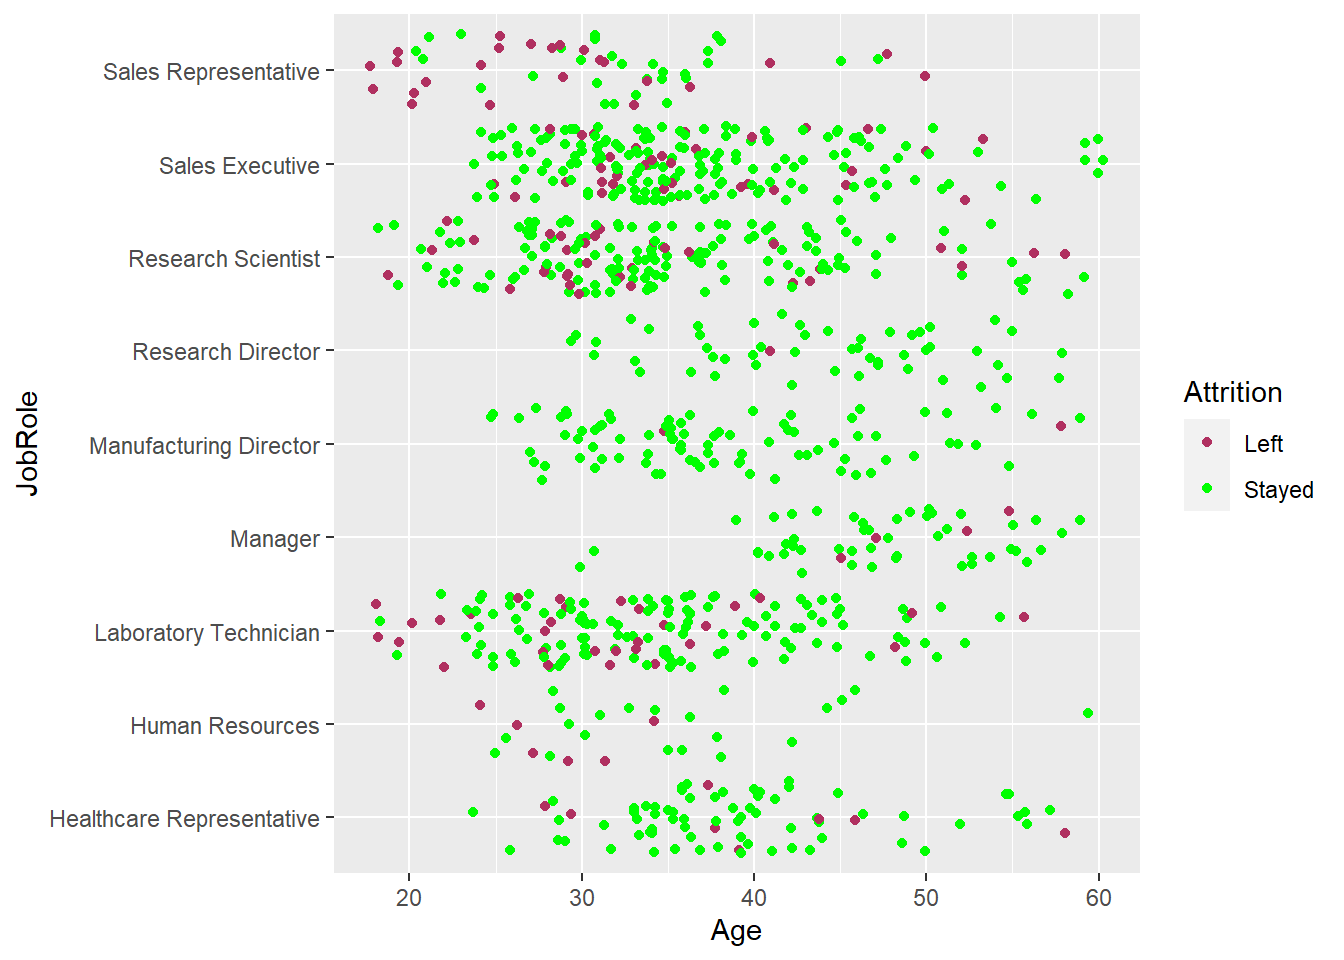
\includegraphics{Employee-Attrition_files/figure-latex/unnamed-chunk-18-1.pdf}

\hypertarget{salary-increase-review}{%
\subsection{Salary Increase Review}\label{salary-increase-review}}

\begin{Shaded}
\begin{Highlighting}[]
\CommentTok{\# Younger Job Roles \#\#\#\#}
\NormalTok{y }\OtherTok{\textless{}{-}} \FunctionTok{filter}\NormalTok{(attrition, JobRole }\SpecialCharTok{==} \StringTok{"Sales Representative"} \SpecialCharTok{|}\NormalTok{ JobRole }\SpecialCharTok{==} \StringTok{"Human Resources"}\NormalTok{) }\SpecialCharTok{\%\textgreater{}\%}
  \FunctionTok{ggplot}\NormalTok{(}\FunctionTok{aes}\NormalTok{(}\AttributeTok{x =}\NormalTok{ PercentSalaryHike, }\AttributeTok{y =}\NormalTok{ JobRole, }\AttributeTok{color =}\NormalTok{ Attrition)) }\SpecialCharTok{+}
  \FunctionTok{geom\_boxplot}\NormalTok{() }\SpecialCharTok{+}
  \FunctionTok{geom\_vline}\NormalTok{(}\FunctionTok{aes}\NormalTok{(}\AttributeTok{xintercept =} \FunctionTok{mean}\NormalTok{(PercentSalaryHike)), }\AttributeTok{color =} \StringTok{"black"}\NormalTok{, }\AttributeTok{linetype =} \StringTok{"dashed"}\NormalTok{) }\SpecialCharTok{+}
  \FunctionTok{ylab}\NormalTok{(}\StringTok{"JobRole"}\NormalTok{) }\SpecialCharTok{+}
  \FunctionTok{xlab}\NormalTok{(}\StringTok{"PercentSalaryHike"}\NormalTok{) }\SpecialCharTok{+}
  \FunctionTok{scale\_color\_manual}\NormalTok{(}\AttributeTok{values =}\NormalTok{ colors) }\SpecialCharTok{+}
  \FunctionTok{ggtitle}\NormalTok{(}\StringTok{"Younger Ages"}\NormalTok{) }\SpecialCharTok{+}
  \FunctionTok{theme}\NormalTok{(}\AttributeTok{legend.position =} \StringTok{"none"}\NormalTok{) }\SpecialCharTok{+}
  \FunctionTok{theme}\NormalTok{(}\AttributeTok{plot.title =} \FunctionTok{element\_text}\NormalTok{(}\AttributeTok{hjust =} \FloatTok{0.5}\NormalTok{)) }
  

\CommentTok{\# OLDER Job Roles \#\#\#\#}
\NormalTok{o }\OtherTok{\textless{}{-}} \FunctionTok{filter}\NormalTok{(attrition, JobRole }\SpecialCharTok{==} \StringTok{"Manager"} \SpecialCharTok{|}\NormalTok{ JobRole }\SpecialCharTok{==} \StringTok{"Research Director"}\NormalTok{ ) }\SpecialCharTok{\%\textgreater{}\%}
  \FunctionTok{ggplot}\NormalTok{(}\FunctionTok{aes}\NormalTok{(}\AttributeTok{x =}\NormalTok{ PercentSalaryHike, }\AttributeTok{y =}\NormalTok{ JobRole, }\AttributeTok{color =}\NormalTok{ Attrition)) }\SpecialCharTok{+}
  \FunctionTok{geom\_boxplot}\NormalTok{() }\SpecialCharTok{+}
  \FunctionTok{geom\_vline}\NormalTok{(}\FunctionTok{aes}\NormalTok{(}\AttributeTok{xintercept =} \FunctionTok{mean}\NormalTok{(PercentSalaryHike)), }\AttributeTok{color =} \StringTok{"black"}\NormalTok{, }\AttributeTok{linetype =} \StringTok{"dashed"}\NormalTok{) }\SpecialCharTok{+}
  \FunctionTok{ylab}\NormalTok{(}\StringTok{"JobRole"}\NormalTok{) }\SpecialCharTok{+}
  \FunctionTok{xlab}\NormalTok{(}\StringTok{"PercentSalaryHike"}\NormalTok{) }\SpecialCharTok{+}
  \FunctionTok{scale\_color\_manual}\NormalTok{(}\AttributeTok{values =}\NormalTok{ colors) }\SpecialCharTok{+}
  \FunctionTok{ggtitle}\NormalTok{(}\StringTok{"Older Ages"}\NormalTok{) }\SpecialCharTok{+}
  \FunctionTok{theme}\NormalTok{(}\AttributeTok{legend.position =} \StringTok{"none"}\NormalTok{) }\SpecialCharTok{+}
  \FunctionTok{theme}\NormalTok{(}\AttributeTok{plot.title =} \FunctionTok{element\_text}\NormalTok{(}\AttributeTok{hjust =} \FloatTok{0.5}\NormalTok{)) }


\CommentTok{\# ALL AGES Job Roles \#\#\#\#}
\NormalTok{a }\OtherTok{\textless{}{-}} \FunctionTok{filter}\NormalTok{(attrition, JobRole }\SpecialCharTok{==} \StringTok{"Research Scientist"} \SpecialCharTok{|}\NormalTok{ JobRole }\SpecialCharTok{==} \StringTok{"Sales Executive"}  \SpecialCharTok{|}\NormalTok{ JobRole }\SpecialCharTok{==} \StringTok{"Laboratory Technician"} \SpecialCharTok{|}\NormalTok{ JobRole }\SpecialCharTok{==} \StringTok{"Healthcare Representative"}\SpecialCharTok{|}\NormalTok{ JobRole }\SpecialCharTok{==} \StringTok{"Manufacturing Director"}\NormalTok{ ) }\SpecialCharTok{\%\textgreater{}\%}
  \FunctionTok{ggplot}\NormalTok{(}\FunctionTok{aes}\NormalTok{(}\AttributeTok{x =}\NormalTok{ PercentSalaryHike, }\AttributeTok{y =}\NormalTok{ JobRole, }\AttributeTok{color =}\NormalTok{ Attrition)) }\SpecialCharTok{+}
  \FunctionTok{geom\_boxplot}\NormalTok{() }\SpecialCharTok{+}
  \FunctionTok{geom\_vline}\NormalTok{(}\FunctionTok{aes}\NormalTok{(}\AttributeTok{xintercept =} \FunctionTok{mean}\NormalTok{(PercentSalaryHike)), }\AttributeTok{color =} \StringTok{"black"}\NormalTok{, }\AttributeTok{linetype =} \StringTok{"dashed"}\NormalTok{) }\SpecialCharTok{+}
  \FunctionTok{ylab}\NormalTok{(}\StringTok{"JobRole"}\NormalTok{) }\SpecialCharTok{+}
  \FunctionTok{xlab}\NormalTok{(}\StringTok{"PercentSalaryHike"}\NormalTok{) }\SpecialCharTok{+}
  \FunctionTok{scale\_color\_manual}\NormalTok{(}\AttributeTok{values =}\NormalTok{ colors) }\SpecialCharTok{+}
  \FunctionTok{ggtitle}\NormalTok{(}\StringTok{"All Ages"}\NormalTok{) }\SpecialCharTok{+}
  \FunctionTok{theme}\NormalTok{(}\AttributeTok{legend.position =} \StringTok{"none"}\NormalTok{) }\SpecialCharTok{+}
  \FunctionTok{theme}\NormalTok{(}\AttributeTok{plot.title =} \FunctionTok{element\_text}\NormalTok{(}\AttributeTok{hjust =} \FloatTok{0.5}\NormalTok{)) }

\FunctionTok{grid.arrange}\NormalTok{(y, o, a, }\AttributeTok{nrow =} \DecValTok{3}\NormalTok{)}
\end{Highlighting}
\end{Shaded}

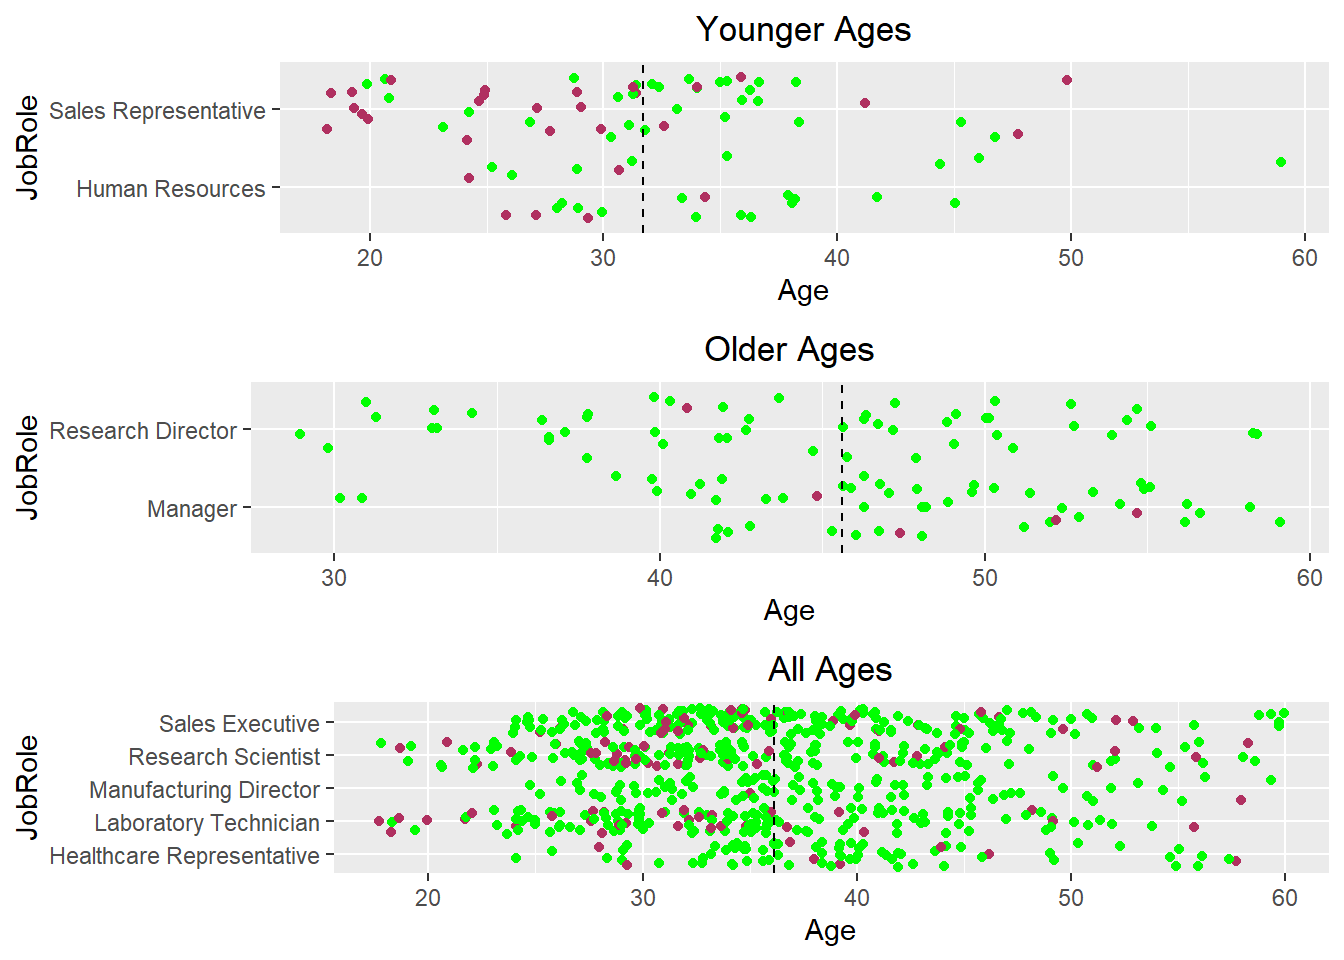
\includegraphics{Employee-Attrition_files/figure-latex/unnamed-chunk-19-1.pdf}

\hypertarget{years-since-last-promotion-review}{%
\subsection{Years Since Last Promotion
Review}\label{years-since-last-promotion-review}}

\begin{Shaded}
\begin{Highlighting}[]
\CommentTok{\# Younger Job Roles \#\#\#\#}
\NormalTok{y }\OtherTok{\textless{}{-}} \FunctionTok{filter}\NormalTok{(attrition, JobRole }\SpecialCharTok{==} \StringTok{"Sales Representative"} \SpecialCharTok{|}\NormalTok{ JobRole }\SpecialCharTok{==} \StringTok{"Human Resources"}\NormalTok{) }\SpecialCharTok{\%\textgreater{}\%}
  \FunctionTok{ggplot}\NormalTok{(}\FunctionTok{aes}\NormalTok{(}\AttributeTok{x =}\NormalTok{ YearsSinceLastPromotion, }\AttributeTok{y =}\NormalTok{ JobRole, }\AttributeTok{color =}\NormalTok{ Attrition)) }\SpecialCharTok{+}
  \FunctionTok{geom\_boxplot}\NormalTok{() }\SpecialCharTok{+}
  \FunctionTok{geom\_vline}\NormalTok{(}\FunctionTok{aes}\NormalTok{(}\AttributeTok{xintercept =} \FunctionTok{mean}\NormalTok{(YearsSinceLastPromotion)), }\AttributeTok{color =} \StringTok{"black"}\NormalTok{, }\AttributeTok{linetype =} \StringTok{"dashed"}\NormalTok{) }\SpecialCharTok{+}
  \FunctionTok{ylab}\NormalTok{(}\StringTok{"JobRole"}\NormalTok{) }\SpecialCharTok{+}
  \FunctionTok{xlab}\NormalTok{(}\StringTok{"YearsSinceLastPromotion"}\NormalTok{) }\SpecialCharTok{+}
  \FunctionTok{scale\_color\_manual}\NormalTok{(}\AttributeTok{values =}\NormalTok{ colors) }\SpecialCharTok{+}
  \FunctionTok{ggtitle}\NormalTok{(}\StringTok{"Younger Ages"}\NormalTok{) }\SpecialCharTok{+}
  \FunctionTok{theme}\NormalTok{(}\AttributeTok{legend.position =} \StringTok{"none"}\NormalTok{) }\SpecialCharTok{+}
  \FunctionTok{theme}\NormalTok{(}\AttributeTok{plot.title =} \FunctionTok{element\_text}\NormalTok{(}\AttributeTok{hjust =} \FloatTok{0.5}\NormalTok{)) }
  

\CommentTok{\# OLDER Job Roles \#\#\#\#}
\NormalTok{o }\OtherTok{\textless{}{-}} \FunctionTok{filter}\NormalTok{(attrition, JobRole }\SpecialCharTok{==} \StringTok{"Manager"} \SpecialCharTok{|}\NormalTok{ JobRole }\SpecialCharTok{==} \StringTok{"Research Director"}\NormalTok{ ) }\SpecialCharTok{\%\textgreater{}\%}
  \FunctionTok{ggplot}\NormalTok{(}\FunctionTok{aes}\NormalTok{(}\AttributeTok{x =}\NormalTok{ YearsSinceLastPromotion, }\AttributeTok{y =}\NormalTok{ JobRole, }\AttributeTok{color =}\NormalTok{ Attrition)) }\SpecialCharTok{+}
  \FunctionTok{geom\_boxplot}\NormalTok{() }\SpecialCharTok{+}
  \FunctionTok{geom\_vline}\NormalTok{(}\FunctionTok{aes}\NormalTok{(}\AttributeTok{xintercept =} \FunctionTok{mean}\NormalTok{(YearsSinceLastPromotion)), }\AttributeTok{color =} \StringTok{"black"}\NormalTok{, }\AttributeTok{linetype =} \StringTok{"dashed"}\NormalTok{) }\SpecialCharTok{+}
  \FunctionTok{ylab}\NormalTok{(}\StringTok{"JobRole"}\NormalTok{) }\SpecialCharTok{+}
  \FunctionTok{xlab}\NormalTok{(}\StringTok{"YearsSinceLastPromotion"}\NormalTok{) }\SpecialCharTok{+}
  \FunctionTok{scale\_color\_manual}\NormalTok{(}\AttributeTok{values =}\NormalTok{ colors) }\SpecialCharTok{+}
  \FunctionTok{ggtitle}\NormalTok{(}\StringTok{"Older Ages"}\NormalTok{) }\SpecialCharTok{+}
  \FunctionTok{theme}\NormalTok{(}\AttributeTok{legend.position =} \StringTok{"none"}\NormalTok{) }\SpecialCharTok{+}
  \FunctionTok{theme}\NormalTok{(}\AttributeTok{plot.title =} \FunctionTok{element\_text}\NormalTok{(}\AttributeTok{hjust =} \FloatTok{0.5}\NormalTok{)) }


\CommentTok{\# ALL AGES Job Roles \#\#\#\#}
\NormalTok{a }\OtherTok{\textless{}{-}} \FunctionTok{filter}\NormalTok{(attrition, JobRole }\SpecialCharTok{==} \StringTok{"Research Scientist"} \SpecialCharTok{|}\NormalTok{ JobRole }\SpecialCharTok{==} \StringTok{"Sales Executive"}  \SpecialCharTok{|}\NormalTok{ JobRole }\SpecialCharTok{==} \StringTok{"Laboratory Technician"} \SpecialCharTok{|}\NormalTok{ JobRole }\SpecialCharTok{==} \StringTok{"Healthcare Representative"}\SpecialCharTok{|}\NormalTok{ JobRole }\SpecialCharTok{==} \StringTok{"Manufacturing Director"}\NormalTok{ ) }\SpecialCharTok{\%\textgreater{}\%}
  \FunctionTok{ggplot}\NormalTok{(}\FunctionTok{aes}\NormalTok{(}\AttributeTok{x =}\NormalTok{ YearsSinceLastPromotion, }\AttributeTok{y =}\NormalTok{ JobRole, }\AttributeTok{color =}\NormalTok{ Attrition)) }\SpecialCharTok{+}
  \FunctionTok{geom\_boxplot}\NormalTok{() }\SpecialCharTok{+}
  \FunctionTok{geom\_vline}\NormalTok{(}\FunctionTok{aes}\NormalTok{(}\AttributeTok{xintercept =} \FunctionTok{mean}\NormalTok{(YearsSinceLastPromotion)), }\AttributeTok{color =} \StringTok{"black"}\NormalTok{, }\AttributeTok{linetype =} \StringTok{"dashed"}\NormalTok{) }\SpecialCharTok{+}
  \FunctionTok{ylab}\NormalTok{(}\StringTok{"JobRole"}\NormalTok{) }\SpecialCharTok{+}
  \FunctionTok{xlab}\NormalTok{(}\StringTok{"YearsSinceLastPromotion"}\NormalTok{) }\SpecialCharTok{+}
  \FunctionTok{scale\_color\_manual}\NormalTok{(}\AttributeTok{values =}\NormalTok{ colors) }\SpecialCharTok{+}
  \FunctionTok{ggtitle}\NormalTok{(}\StringTok{"All Ages"}\NormalTok{) }\SpecialCharTok{+}
  \FunctionTok{theme}\NormalTok{(}\AttributeTok{legend.position =} \StringTok{"none"}\NormalTok{) }\SpecialCharTok{+}
  \FunctionTok{theme}\NormalTok{(}\AttributeTok{plot.title =} \FunctionTok{element\_text}\NormalTok{(}\AttributeTok{hjust =} \FloatTok{0.5}\NormalTok{)) }

\FunctionTok{grid.arrange}\NormalTok{(y, o, a, }\AttributeTok{nrow =} \DecValTok{3}\NormalTok{)}
\end{Highlighting}
\end{Shaded}

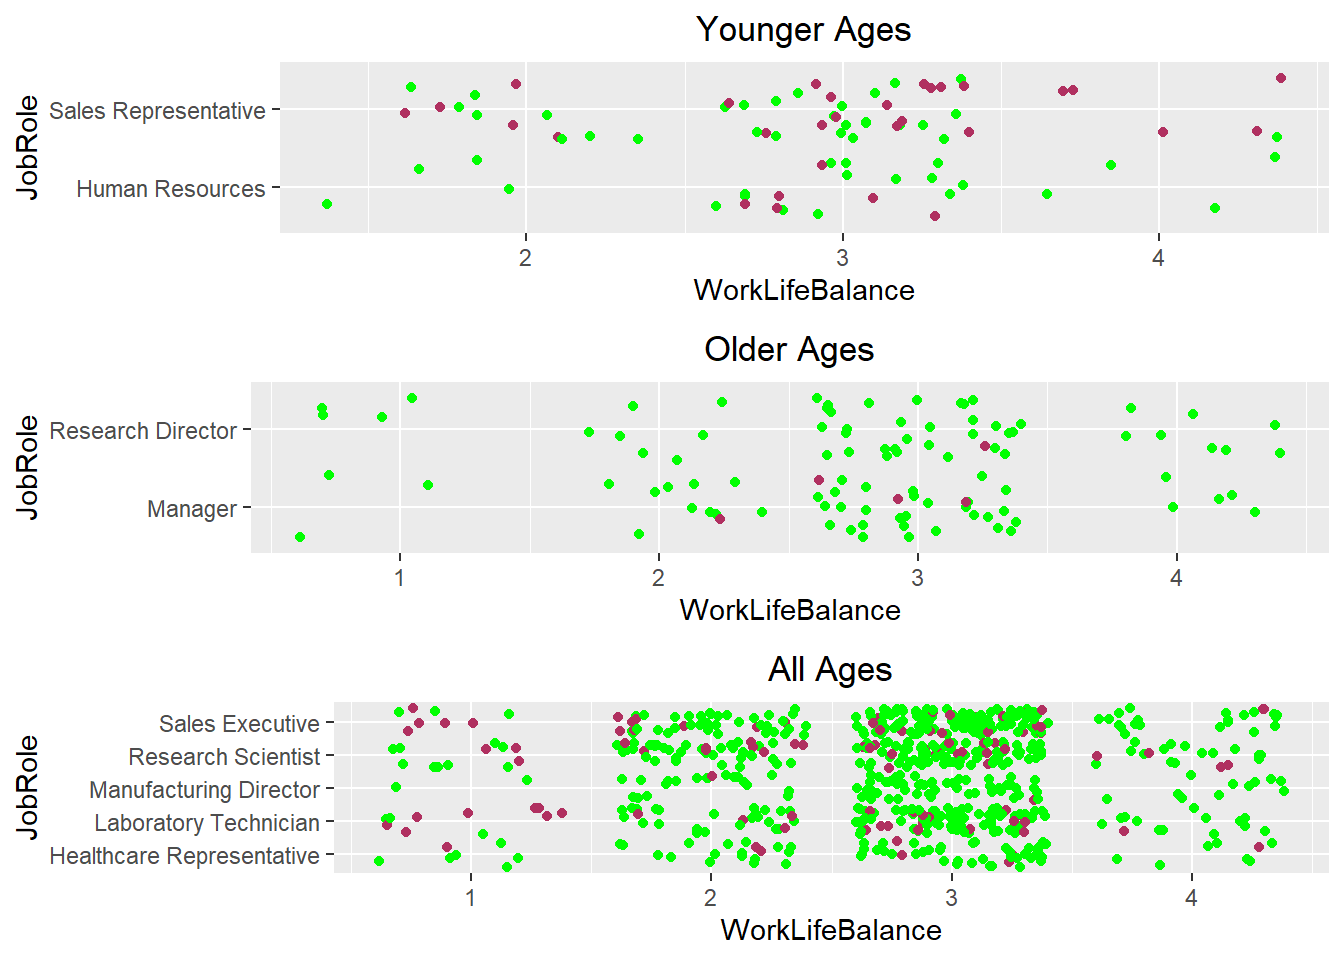
\includegraphics{Employee-Attrition_files/figure-latex/unnamed-chunk-20-1.pdf}

\begin{Shaded}
\begin{Highlighting}[]
\CommentTok{\# Younger Job Roles \#\#\#\#}
\NormalTok{y }\OtherTok{\textless{}{-}} \FunctionTok{filter}\NormalTok{(attrition, JobRole }\SpecialCharTok{==} \StringTok{"Sales Representative"} \SpecialCharTok{|}\NormalTok{ JobRole }\SpecialCharTok{==} \StringTok{"Human Resources"}\NormalTok{) }\SpecialCharTok{\%\textgreater{}\%}
  \FunctionTok{ggplot}\NormalTok{(}\FunctionTok{aes}\NormalTok{(}\AttributeTok{x =}\NormalTok{ YearsInCurrentRole, }\AttributeTok{y =}\NormalTok{ JobRole, }\AttributeTok{color =}\NormalTok{ Attrition)) }\SpecialCharTok{+}
  \FunctionTok{geom\_boxplot}\NormalTok{() }\SpecialCharTok{+}
  \FunctionTok{geom\_vline}\NormalTok{(}\FunctionTok{aes}\NormalTok{(}\AttributeTok{xintercept =} \FunctionTok{mean}\NormalTok{(YearsInCurrentRole)), }\AttributeTok{color =} \StringTok{"black"}\NormalTok{, }\AttributeTok{linetype =} \StringTok{"dashed"}\NormalTok{) }\SpecialCharTok{+}
  \FunctionTok{ylab}\NormalTok{(}\StringTok{"JobRole"}\NormalTok{) }\SpecialCharTok{+}
  \FunctionTok{xlab}\NormalTok{(}\StringTok{"YearsInCurrentRole"}\NormalTok{) }\SpecialCharTok{+}
  \FunctionTok{scale\_color\_manual}\NormalTok{(}\AttributeTok{values =}\NormalTok{ colors) }\SpecialCharTok{+}
  \FunctionTok{ggtitle}\NormalTok{(}\StringTok{"Younger Ages"}\NormalTok{) }\SpecialCharTok{+}
  \FunctionTok{theme}\NormalTok{(}\AttributeTok{legend.position =} \StringTok{"none"}\NormalTok{) }\SpecialCharTok{+}
  \FunctionTok{theme}\NormalTok{(}\AttributeTok{plot.title =} \FunctionTok{element\_text}\NormalTok{(}\AttributeTok{hjust =} \FloatTok{0.5}\NormalTok{)) }
  

\CommentTok{\# OLDER Job Roles \#\#\#\#}
\NormalTok{o }\OtherTok{\textless{}{-}} \FunctionTok{filter}\NormalTok{(attrition, JobRole }\SpecialCharTok{==} \StringTok{"Manager"} \SpecialCharTok{|}\NormalTok{ JobRole }\SpecialCharTok{==} \StringTok{"Research Director"}\NormalTok{ ) }\SpecialCharTok{\%\textgreater{}\%}
  \FunctionTok{ggplot}\NormalTok{(}\FunctionTok{aes}\NormalTok{(}\AttributeTok{x =}\NormalTok{ YearsInCurrentRole, }\AttributeTok{y =}\NormalTok{ JobRole, }\AttributeTok{color =}\NormalTok{ Attrition)) }\SpecialCharTok{+}
  \FunctionTok{geom\_boxplot}\NormalTok{() }\SpecialCharTok{+}
  \FunctionTok{geom\_vline}\NormalTok{(}\FunctionTok{aes}\NormalTok{(}\AttributeTok{xintercept =} \FunctionTok{mean}\NormalTok{(YearsInCurrentRole)), }\AttributeTok{color =} \StringTok{"black"}\NormalTok{, }\AttributeTok{linetype =} \StringTok{"dashed"}\NormalTok{) }\SpecialCharTok{+}
  \FunctionTok{ylab}\NormalTok{(}\StringTok{"JobRole"}\NormalTok{) }\SpecialCharTok{+}
  \FunctionTok{xlab}\NormalTok{(}\StringTok{"YearsInCurrentRole"}\NormalTok{) }\SpecialCharTok{+}
  \FunctionTok{scale\_color\_manual}\NormalTok{(}\AttributeTok{values =}\NormalTok{ colors) }\SpecialCharTok{+}
  \FunctionTok{ggtitle}\NormalTok{(}\StringTok{"Older Ages"}\NormalTok{) }\SpecialCharTok{+}
  \FunctionTok{theme}\NormalTok{(}\AttributeTok{legend.position =} \StringTok{"none"}\NormalTok{) }\SpecialCharTok{+}
  \FunctionTok{theme}\NormalTok{(}\AttributeTok{plot.title =} \FunctionTok{element\_text}\NormalTok{(}\AttributeTok{hjust =} \FloatTok{0.5}\NormalTok{)) }


\CommentTok{\# ALL AGES Job Roles \#\#\#\#}
\NormalTok{a }\OtherTok{\textless{}{-}} \FunctionTok{filter}\NormalTok{(attrition, JobRole }\SpecialCharTok{==} \StringTok{"Research Scientist"} \SpecialCharTok{|}\NormalTok{ JobRole }\SpecialCharTok{==} \StringTok{"Sales Executive"}  \SpecialCharTok{|}\NormalTok{ JobRole }\SpecialCharTok{==} \StringTok{"Laboratory Technician"} \SpecialCharTok{|}\NormalTok{ JobRole }\SpecialCharTok{==} \StringTok{"Healthcare Representative"}\SpecialCharTok{|}\NormalTok{ JobRole }\SpecialCharTok{==} \StringTok{"Manufacturing Director"}\NormalTok{ ) }\SpecialCharTok{\%\textgreater{}\%}
  \FunctionTok{ggplot}\NormalTok{(}\FunctionTok{aes}\NormalTok{(}\AttributeTok{x =}\NormalTok{ YearsInCurrentRole, }\AttributeTok{y =}\NormalTok{ JobRole, }\AttributeTok{color =}\NormalTok{ Attrition)) }\SpecialCharTok{+}
  \FunctionTok{geom\_boxplot}\NormalTok{() }\SpecialCharTok{+}
  \FunctionTok{geom\_vline}\NormalTok{(}\FunctionTok{aes}\NormalTok{(}\AttributeTok{xintercept =} \FunctionTok{mean}\NormalTok{(YearsInCurrentRole)), }\AttributeTok{color =} \StringTok{"black"}\NormalTok{, }\AttributeTok{linetype =} \StringTok{"dashed"}\NormalTok{) }\SpecialCharTok{+}
  \FunctionTok{ylab}\NormalTok{(}\StringTok{"JobRole"}\NormalTok{) }\SpecialCharTok{+}
  \FunctionTok{xlab}\NormalTok{(}\StringTok{"YearsInCurrentRole"}\NormalTok{) }\SpecialCharTok{+}
  \FunctionTok{scale\_color\_manual}\NormalTok{(}\AttributeTok{values =}\NormalTok{ colors) }\SpecialCharTok{+}
  \FunctionTok{ggtitle}\NormalTok{(}\StringTok{"All Ages"}\NormalTok{) }\SpecialCharTok{+}
  \FunctionTok{theme}\NormalTok{(}\AttributeTok{legend.position =} \StringTok{"none"}\NormalTok{) }\SpecialCharTok{+}
  \FunctionTok{theme}\NormalTok{(}\AttributeTok{plot.title =} \FunctionTok{element\_text}\NormalTok{(}\AttributeTok{hjust =} \FloatTok{0.5}\NormalTok{)) }

\FunctionTok{grid.arrange}\NormalTok{(y, o, a, }\AttributeTok{nrow =} \DecValTok{3}\NormalTok{)}
\end{Highlighting}
\end{Shaded}

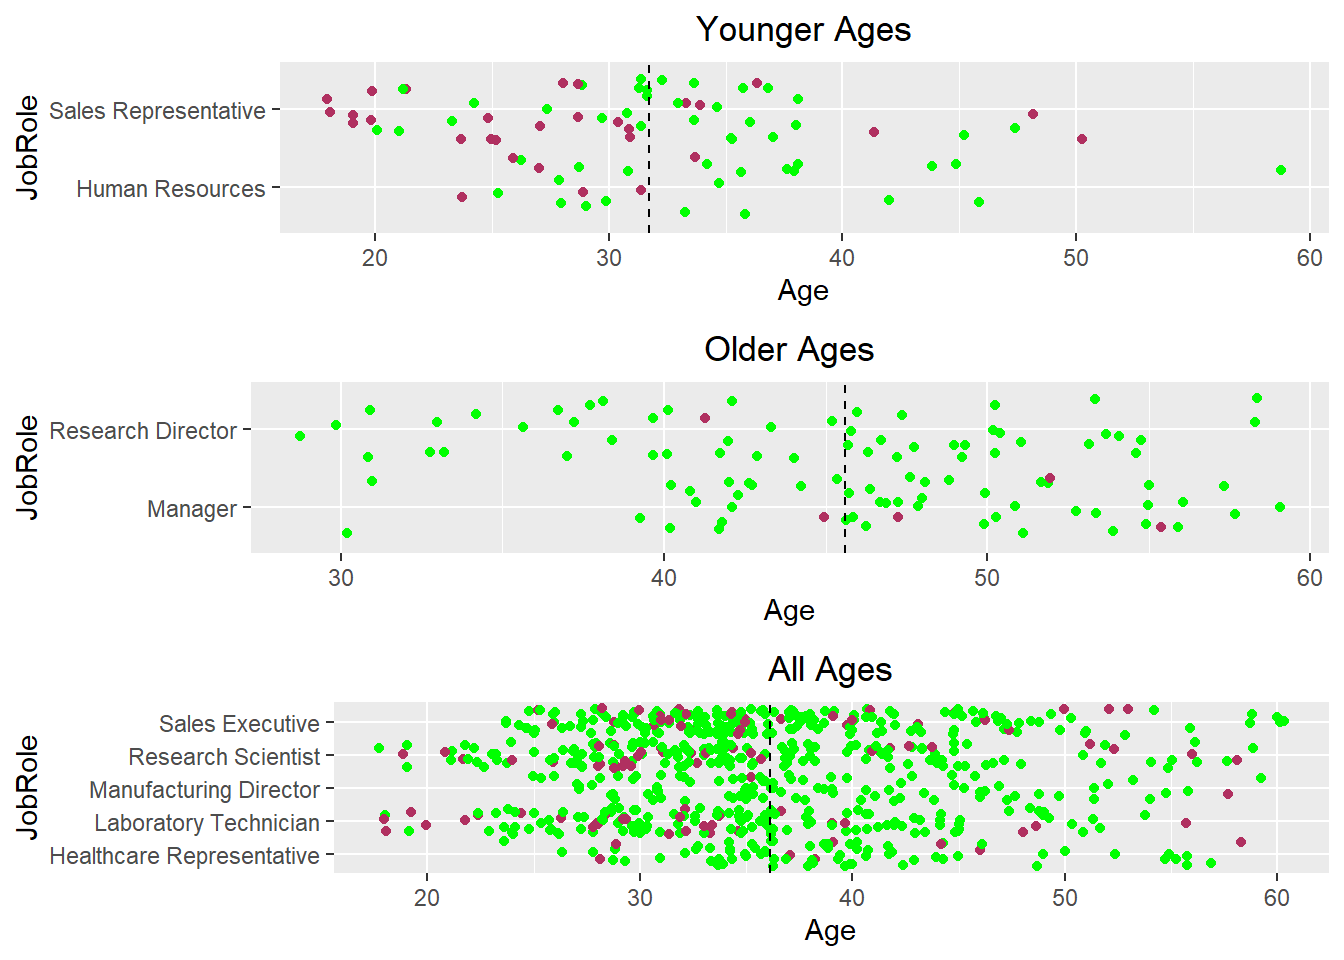
\includegraphics{Employee-Attrition_files/figure-latex/unnamed-chunk-21-1.pdf}

\hypertarget{gender-review}{%
\subsection{Gender Review}\label{gender-review}}

\begin{Shaded}
\begin{Highlighting}[]
\CommentTok{\# Younger Job Roles \#\#\#\#}
\NormalTok{y }\OtherTok{\textless{}{-}} \FunctionTok{filter}\NormalTok{(attrition, JobRole }\SpecialCharTok{==} \StringTok{"Sales Representative"} \SpecialCharTok{|}\NormalTok{ JobRole }\SpecialCharTok{==} \StringTok{"Human Resources"}\NormalTok{) }\SpecialCharTok{\%\textgreater{}\%}
  \FunctionTok{ggplot}\NormalTok{(}\FunctionTok{aes}\NormalTok{(}\AttributeTok{x =}\NormalTok{ Gender, }\AttributeTok{y =}\NormalTok{ JobRole, }\AttributeTok{color =}\NormalTok{ Attrition)) }\SpecialCharTok{+}
  \FunctionTok{geom\_point}\NormalTok{(}\AttributeTok{position =} \StringTok{"jitter"}\NormalTok{) }\SpecialCharTok{+}
  \FunctionTok{ylab}\NormalTok{(}\StringTok{"JobRole"}\NormalTok{) }\SpecialCharTok{+}
  \FunctionTok{xlab}\NormalTok{(}\StringTok{"Gender"}\NormalTok{) }\SpecialCharTok{+}
  \FunctionTok{scale\_color\_manual}\NormalTok{(}\AttributeTok{values =}\NormalTok{ colors) }\SpecialCharTok{+}
  \FunctionTok{ggtitle}\NormalTok{(}\StringTok{"Younger Ages"}\NormalTok{) }\SpecialCharTok{+}
  \FunctionTok{theme}\NormalTok{(}\AttributeTok{legend.position =} \StringTok{"none"}\NormalTok{) }\SpecialCharTok{+}
  \FunctionTok{theme}\NormalTok{(}\AttributeTok{plot.title =} \FunctionTok{element\_text}\NormalTok{(}\AttributeTok{hjust =} \FloatTok{0.5}\NormalTok{)) }
  

\CommentTok{\# OLDER Job Roles \#\#\#\#}
\NormalTok{o }\OtherTok{\textless{}{-}} \FunctionTok{filter}\NormalTok{(attrition, JobRole }\SpecialCharTok{==} \StringTok{"Manager"} \SpecialCharTok{|}\NormalTok{ JobRole }\SpecialCharTok{==} \StringTok{"Research Director"}\NormalTok{ ) }\SpecialCharTok{\%\textgreater{}\%}
  \FunctionTok{ggplot}\NormalTok{(}\FunctionTok{aes}\NormalTok{(}\AttributeTok{x =}\NormalTok{ Gender, }\AttributeTok{y =}\NormalTok{ JobRole, }\AttributeTok{color =}\NormalTok{ Attrition)) }\SpecialCharTok{+}
  \FunctionTok{geom\_point}\NormalTok{(}\AttributeTok{position =} \StringTok{"jitter"}\NormalTok{) }\SpecialCharTok{+}
  \FunctionTok{ylab}\NormalTok{(}\StringTok{"JobRole"}\NormalTok{) }\SpecialCharTok{+}
  \FunctionTok{xlab}\NormalTok{(}\StringTok{"Gender"}\NormalTok{) }\SpecialCharTok{+}
  \FunctionTok{scale\_color\_manual}\NormalTok{(}\AttributeTok{values =}\NormalTok{ colors) }\SpecialCharTok{+}
  \FunctionTok{ggtitle}\NormalTok{(}\StringTok{"Older Ages"}\NormalTok{) }\SpecialCharTok{+}
  \FunctionTok{theme}\NormalTok{(}\AttributeTok{legend.position =} \StringTok{"none"}\NormalTok{) }\SpecialCharTok{+}
  \FunctionTok{theme}\NormalTok{(}\AttributeTok{plot.title =} \FunctionTok{element\_text}\NormalTok{(}\AttributeTok{hjust =} \FloatTok{0.5}\NormalTok{)) }


\CommentTok{\# ALL AGES Job Roles \#\#\#\#}
\NormalTok{a }\OtherTok{\textless{}{-}} \FunctionTok{filter}\NormalTok{(attrition, JobRole }\SpecialCharTok{==} \StringTok{"Research Scientist"} \SpecialCharTok{|}\NormalTok{ JobRole }\SpecialCharTok{==} \StringTok{"Sales Executive"}  \SpecialCharTok{|}\NormalTok{ JobRole }\SpecialCharTok{==} \StringTok{"Laboratory Technician"} \SpecialCharTok{|}\NormalTok{ JobRole }\SpecialCharTok{==} \StringTok{"Healthcare Representative"}\SpecialCharTok{|}\NormalTok{ JobRole }\SpecialCharTok{==} \StringTok{"Manufacturing Director"}\NormalTok{ ) }\SpecialCharTok{\%\textgreater{}\%}
  \FunctionTok{ggplot}\NormalTok{(}\FunctionTok{aes}\NormalTok{(}\AttributeTok{x =}\NormalTok{ Gender, }\AttributeTok{y =}\NormalTok{ JobRole, }\AttributeTok{color =}\NormalTok{ Attrition)) }\SpecialCharTok{+}
  \FunctionTok{geom\_point}\NormalTok{(}\AttributeTok{position =} \StringTok{"jitter"}\NormalTok{) }\SpecialCharTok{+}
  \FunctionTok{ylab}\NormalTok{(}\StringTok{"JobRole"}\NormalTok{) }\SpecialCharTok{+}
  \FunctionTok{xlab}\NormalTok{(}\StringTok{"Gender"}\NormalTok{) }\SpecialCharTok{+}
  \FunctionTok{scale\_color\_manual}\NormalTok{(}\AttributeTok{values =}\NormalTok{ colors) }\SpecialCharTok{+}
  \FunctionTok{ggtitle}\NormalTok{(}\StringTok{"All Ages"}\NormalTok{) }\SpecialCharTok{+}
  \FunctionTok{theme}\NormalTok{(}\AttributeTok{legend.position =} \StringTok{"none"}\NormalTok{) }\SpecialCharTok{+}
  \FunctionTok{theme}\NormalTok{(}\AttributeTok{plot.title =} \FunctionTok{element\_text}\NormalTok{(}\AttributeTok{hjust =} \FloatTok{0.5}\NormalTok{)) }

\FunctionTok{grid.arrange}\NormalTok{(y, o, a, }\AttributeTok{nrow =} \DecValTok{3}\NormalTok{)}
\end{Highlighting}
\end{Shaded}

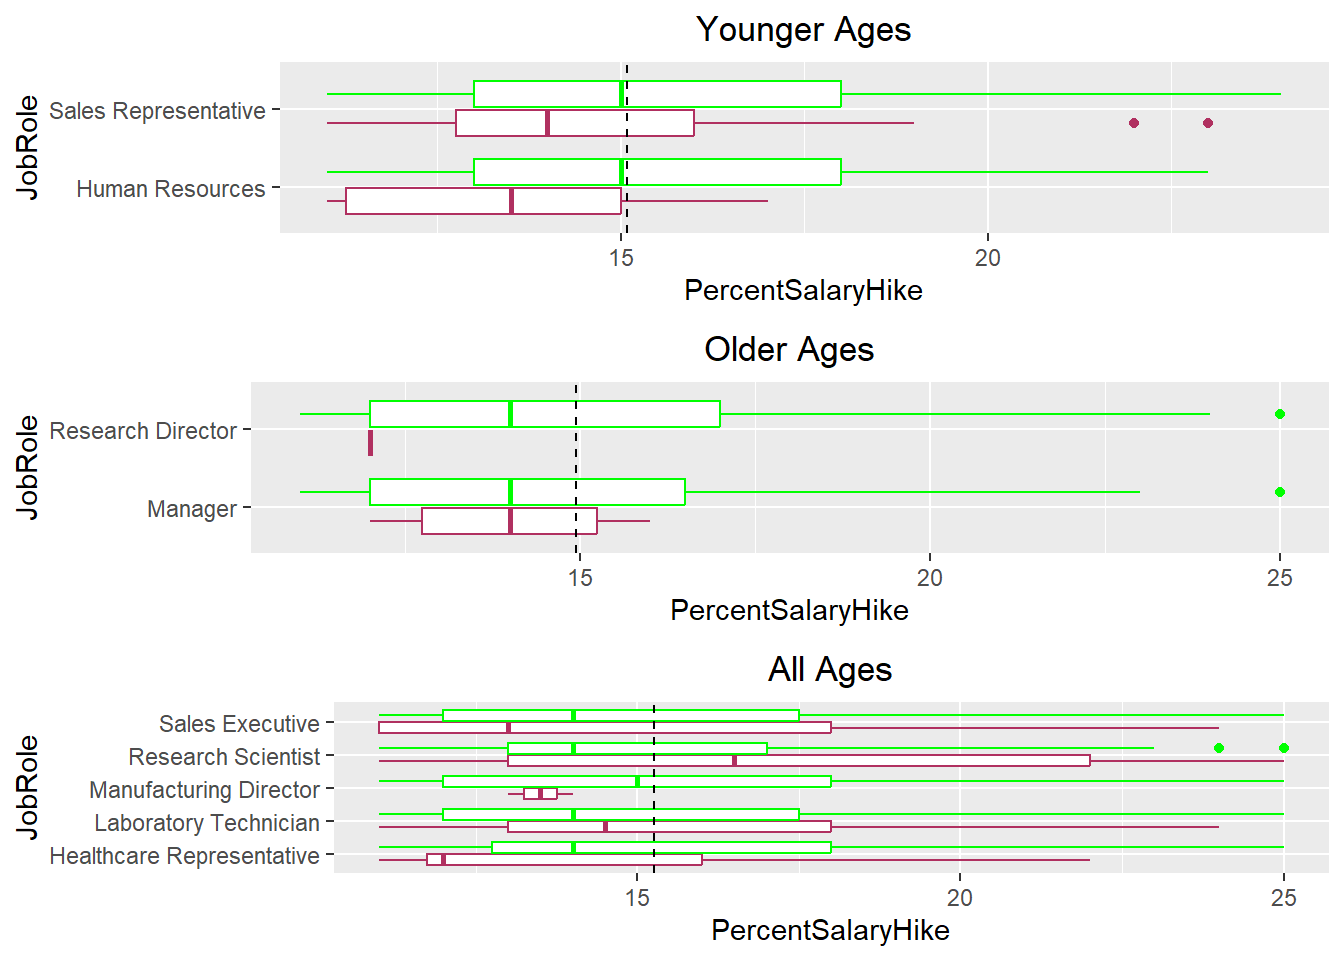
\includegraphics{Employee-Attrition_files/figure-latex/unnamed-chunk-22-1.pdf}

\hypertarget{younger-job-role-review}{%
\subsection{Younger Job Role Review}\label{younger-job-role-review}}

\begin{Shaded}
\begin{Highlighting}[]
\CommentTok{\# Training Times Last Year \#\#\#\#}
\FunctionTok{filter}\NormalTok{(attrition, JobRole }\SpecialCharTok{==} \StringTok{"Sales Representative"} \SpecialCharTok{|}\NormalTok{ JobRole }\SpecialCharTok{==} \StringTok{"Human Resources"}\NormalTok{) }\SpecialCharTok{\%\textgreater{}\%}
  \FunctionTok{ggplot}\NormalTok{(}\FunctionTok{aes}\NormalTok{(}\AttributeTok{x =}\NormalTok{ TrainingTimesLastYear, }\AttributeTok{y =}\NormalTok{ JobRole, }\AttributeTok{color =}\NormalTok{ Attrition)) }\SpecialCharTok{+}
  \FunctionTok{geom\_boxplot}\NormalTok{() }\SpecialCharTok{+}
  \FunctionTok{geom\_vline}\NormalTok{(}\FunctionTok{aes}\NormalTok{(}\AttributeTok{xintercept =} \FunctionTok{mean}\NormalTok{(TrainingTimesLastYear)), }\AttributeTok{color =} \StringTok{"black"}\NormalTok{, }\AttributeTok{linetype =} \StringTok{"dashed"}\NormalTok{) }\SpecialCharTok{+}
  \FunctionTok{ylab}\NormalTok{(}\StringTok{"JobRole"}\NormalTok{) }\SpecialCharTok{+}
  \FunctionTok{xlab}\NormalTok{(}\StringTok{"TrainingTimesLastYear"}\NormalTok{) }\SpecialCharTok{+}
  \FunctionTok{ggtitle}\NormalTok{(}\StringTok{"Training Times Last Year"}\NormalTok{) }\SpecialCharTok{+}
  \FunctionTok{scale\_color\_manual}\NormalTok{(}\AttributeTok{values =}\NormalTok{ colors) }\SpecialCharTok{+}
  \FunctionTok{theme}\NormalTok{(}\AttributeTok{legend.position =} \StringTok{"none"}\NormalTok{) }\SpecialCharTok{+}
  \FunctionTok{theme}\NormalTok{(}\AttributeTok{plot.title =} \FunctionTok{element\_text}\NormalTok{(}\AttributeTok{hjust =} \FloatTok{0.5}\NormalTok{)) }
\end{Highlighting}
\end{Shaded}

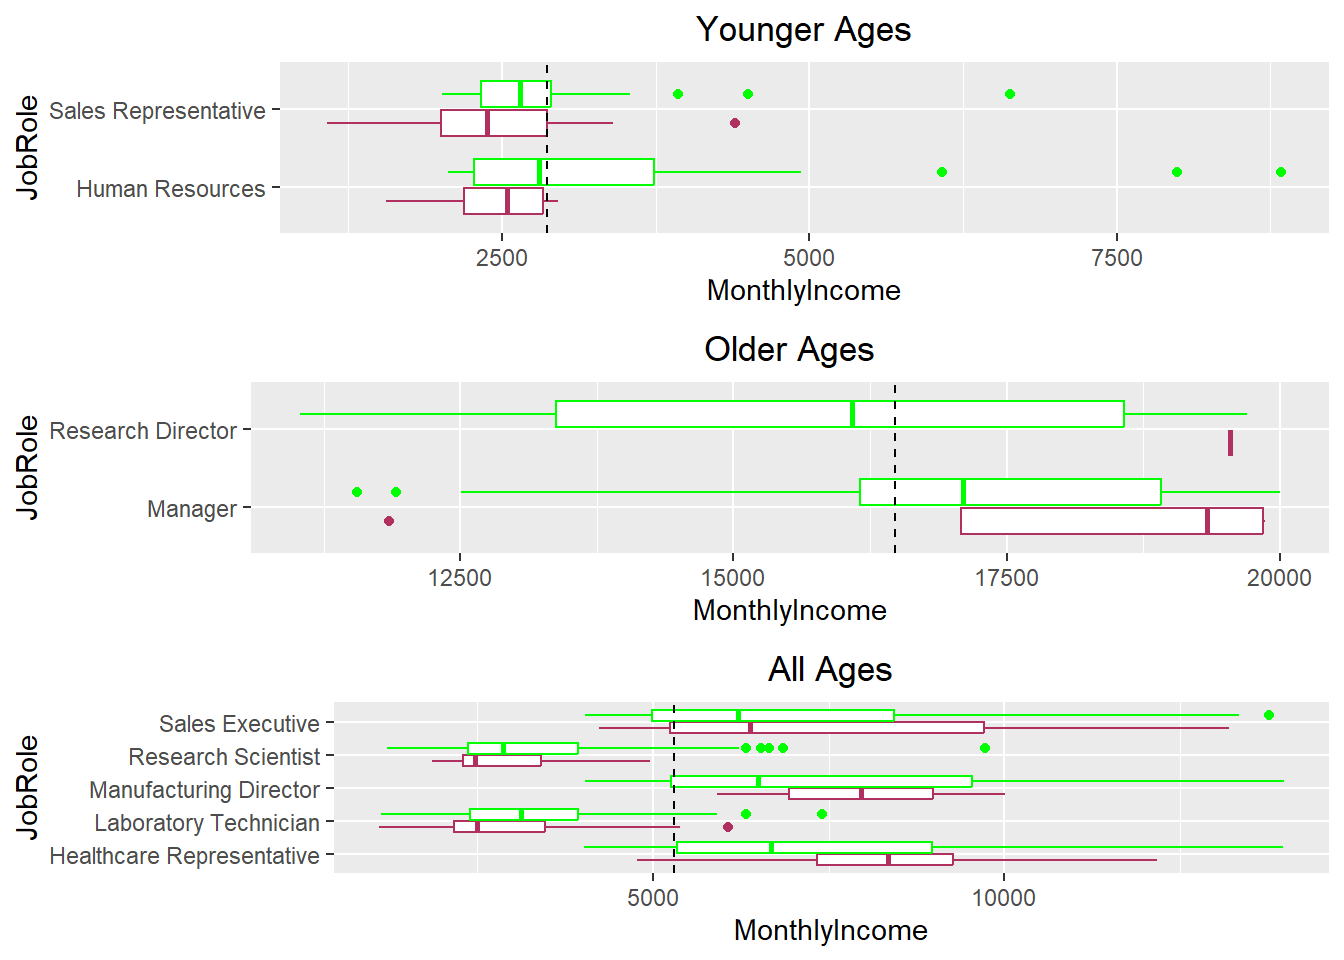
\includegraphics{Employee-Attrition_files/figure-latex/unnamed-chunk-23-1.pdf}

\begin{Shaded}
\begin{Highlighting}[]
\CommentTok{\# Education \#\#\#\#}
\FunctionTok{filter}\NormalTok{(attrition, JobRole }\SpecialCharTok{==} \StringTok{"Sales Representative"} \SpecialCharTok{|}\NormalTok{ JobRole }\SpecialCharTok{==} \StringTok{"Human Resources"}\NormalTok{) }\SpecialCharTok{\%\textgreater{}\%}
  \FunctionTok{ggplot}\NormalTok{(}\FunctionTok{aes}\NormalTok{(}\AttributeTok{x =}\NormalTok{ Education, }\AttributeTok{y =}\NormalTok{ JobRole, }\AttributeTok{color =}\NormalTok{ Attrition)) }\SpecialCharTok{+}
  \FunctionTok{geom\_boxplot}\NormalTok{() }\SpecialCharTok{+}
  \FunctionTok{geom\_vline}\NormalTok{(}\FunctionTok{aes}\NormalTok{(}\AttributeTok{xintercept =} \FunctionTok{mean}\NormalTok{(Education)), }\AttributeTok{color =} \StringTok{"black"}\NormalTok{, }\AttributeTok{linetype =} \StringTok{"dashed"}\NormalTok{) }\SpecialCharTok{+}
  \FunctionTok{ylab}\NormalTok{(}\StringTok{"JobRole"}\NormalTok{) }\SpecialCharTok{+}
  \FunctionTok{xlab}\NormalTok{(}\StringTok{"Education"}\NormalTok{) }\SpecialCharTok{+}
  \FunctionTok{ggtitle}\NormalTok{(}\StringTok{"Education"}\NormalTok{) }\SpecialCharTok{+}
  \FunctionTok{scale\_color\_manual}\NormalTok{(}\AttributeTok{values =}\NormalTok{ colors) }\SpecialCharTok{+}
  \FunctionTok{theme}\NormalTok{(}\AttributeTok{legend.position =} \StringTok{"none"}\NormalTok{) }\SpecialCharTok{+}
  \FunctionTok{theme}\NormalTok{(}\AttributeTok{plot.title =} \FunctionTok{element\_text}\NormalTok{(}\AttributeTok{hjust =} \FloatTok{0.5}\NormalTok{)) }
\end{Highlighting}
\end{Shaded}

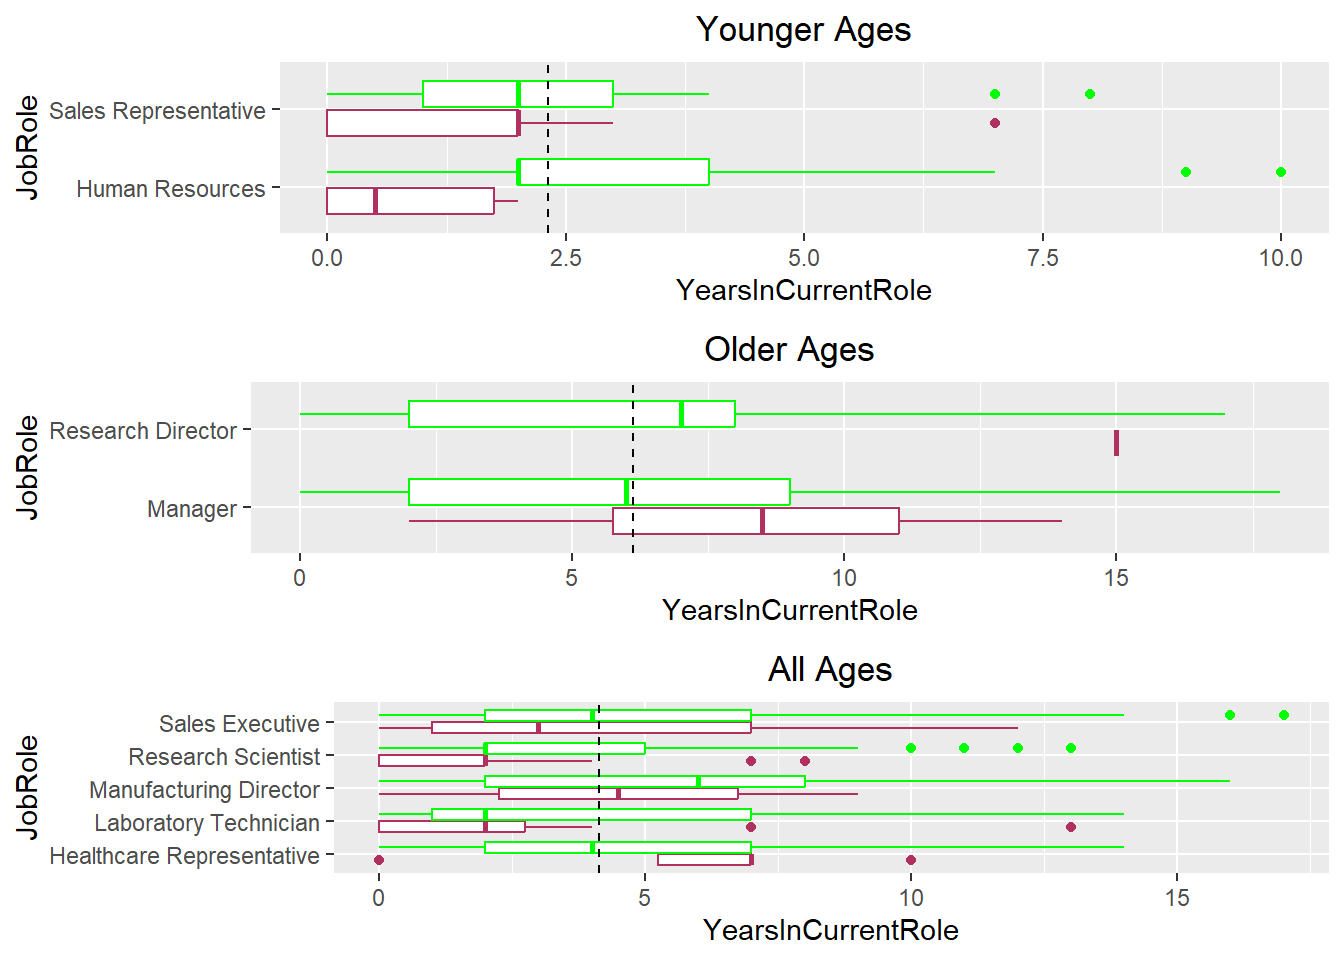
\includegraphics{Employee-Attrition_files/figure-latex/unnamed-chunk-24-1.pdf}

\begin{Shaded}
\begin{Highlighting}[]
\CommentTok{\# Distance From Home \#\#\#\#}
\FunctionTok{filter}\NormalTok{(attrition, JobRole }\SpecialCharTok{==} \StringTok{"Sales Representative"} \SpecialCharTok{|}\NormalTok{ JobRole }\SpecialCharTok{==} \StringTok{"Human Resources"}\NormalTok{) }\SpecialCharTok{\%\textgreater{}\%}
  \FunctionTok{ggplot}\NormalTok{(}\FunctionTok{aes}\NormalTok{(}\AttributeTok{x =}\NormalTok{ DistanceFromHome, }\AttributeTok{y =}\NormalTok{ JobRole, }\AttributeTok{color =}\NormalTok{ Attrition)) }\SpecialCharTok{+}
  \FunctionTok{geom\_boxplot}\NormalTok{() }\SpecialCharTok{+}
  \FunctionTok{geom\_vline}\NormalTok{(}\FunctionTok{aes}\NormalTok{(}\AttributeTok{xintercept =} \FunctionTok{mean}\NormalTok{(DistanceFromHome)), }\AttributeTok{color =} \StringTok{"black"}\NormalTok{, }\AttributeTok{linetype =} \StringTok{"dashed"}\NormalTok{) }\SpecialCharTok{+}
  \FunctionTok{ylab}\NormalTok{(}\StringTok{"JobRole"}\NormalTok{) }\SpecialCharTok{+}
  \FunctionTok{xlab}\NormalTok{(}\StringTok{"DistanceFromHome"}\NormalTok{) }\SpecialCharTok{+}
  \FunctionTok{ggtitle}\NormalTok{(}\StringTok{"Distance From Home"}\NormalTok{) }\SpecialCharTok{+}
  \FunctionTok{scale\_color\_manual}\NormalTok{(}\AttributeTok{values =}\NormalTok{ colors) }\SpecialCharTok{+}
  \FunctionTok{theme}\NormalTok{(}\AttributeTok{legend.position =} \StringTok{"none"}\NormalTok{) }\SpecialCharTok{+}
  \FunctionTok{theme}\NormalTok{(}\AttributeTok{plot.title =} \FunctionTok{element\_text}\NormalTok{(}\AttributeTok{hjust =} \FloatTok{0.5}\NormalTok{)) }
\end{Highlighting}
\end{Shaded}

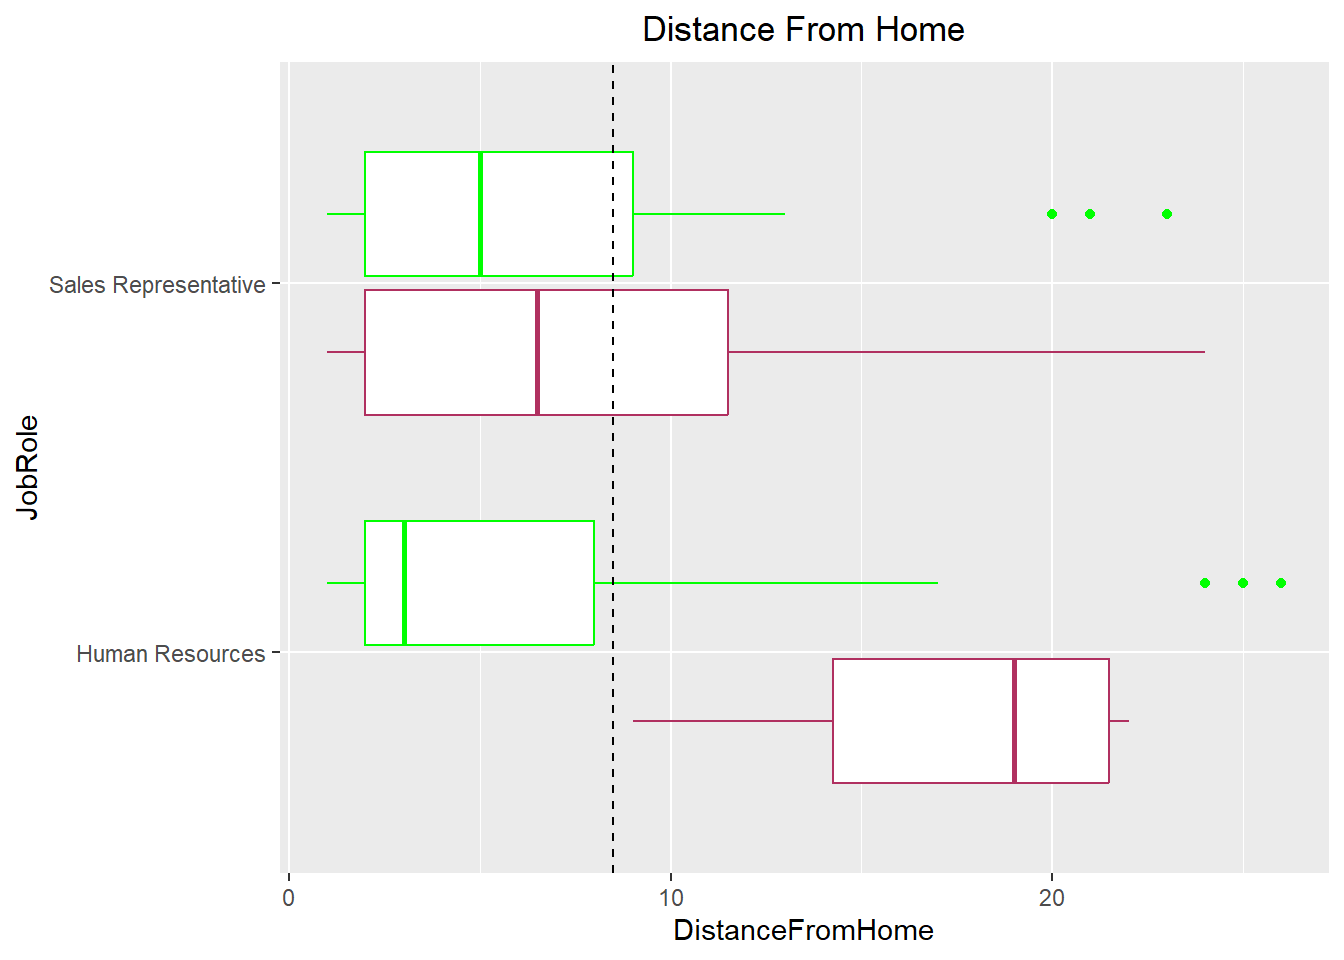
\includegraphics{Employee-Attrition_files/figure-latex/unnamed-chunk-25-1.pdf}

\begin{Shaded}
\begin{Highlighting}[]
\CommentTok{\# Years in Current Role \#\#\#\#}
\FunctionTok{filter}\NormalTok{(attrition, JobRole }\SpecialCharTok{==} \StringTok{"Sales Representative"} \SpecialCharTok{|}\NormalTok{ JobRole }\SpecialCharTok{==} \StringTok{"Human Resources"}\NormalTok{) }\SpecialCharTok{\%\textgreater{}\%}
  \FunctionTok{ggplot}\NormalTok{(}\FunctionTok{aes}\NormalTok{(}\AttributeTok{x =}\NormalTok{ YearsInCurrentRole, }\AttributeTok{y =}\NormalTok{ JobRole, }\AttributeTok{color =}\NormalTok{ Attrition)) }\SpecialCharTok{+}
  \FunctionTok{geom\_boxplot}\NormalTok{() }\SpecialCharTok{+}
  \FunctionTok{geom\_vline}\NormalTok{(}\FunctionTok{aes}\NormalTok{(}\AttributeTok{xintercept =} \FunctionTok{mean}\NormalTok{(YearsInCurrentRole)), }\AttributeTok{color =} \StringTok{"black"}\NormalTok{, }\AttributeTok{linetype =} \StringTok{"dashed"}\NormalTok{) }\SpecialCharTok{+}
  \FunctionTok{ylab}\NormalTok{(}\StringTok{"JobRole"}\NormalTok{) }\SpecialCharTok{+}
  \FunctionTok{xlab}\NormalTok{(}\StringTok{"YearsInCurrentRole"}\NormalTok{) }\SpecialCharTok{+}
  \FunctionTok{ggtitle}\NormalTok{(}\StringTok{"Years In Current Role"}\NormalTok{) }\SpecialCharTok{+}
  \FunctionTok{scale\_color\_manual}\NormalTok{(}\AttributeTok{values =}\NormalTok{ colors) }\SpecialCharTok{+}
  \FunctionTok{theme}\NormalTok{(}\AttributeTok{legend.position =} \StringTok{"none"}\NormalTok{) }\SpecialCharTok{+}
  \FunctionTok{theme}\NormalTok{(}\AttributeTok{plot.title =} \FunctionTok{element\_text}\NormalTok{(}\AttributeTok{hjust =} \FloatTok{0.5}\NormalTok{)) }
\end{Highlighting}
\end{Shaded}

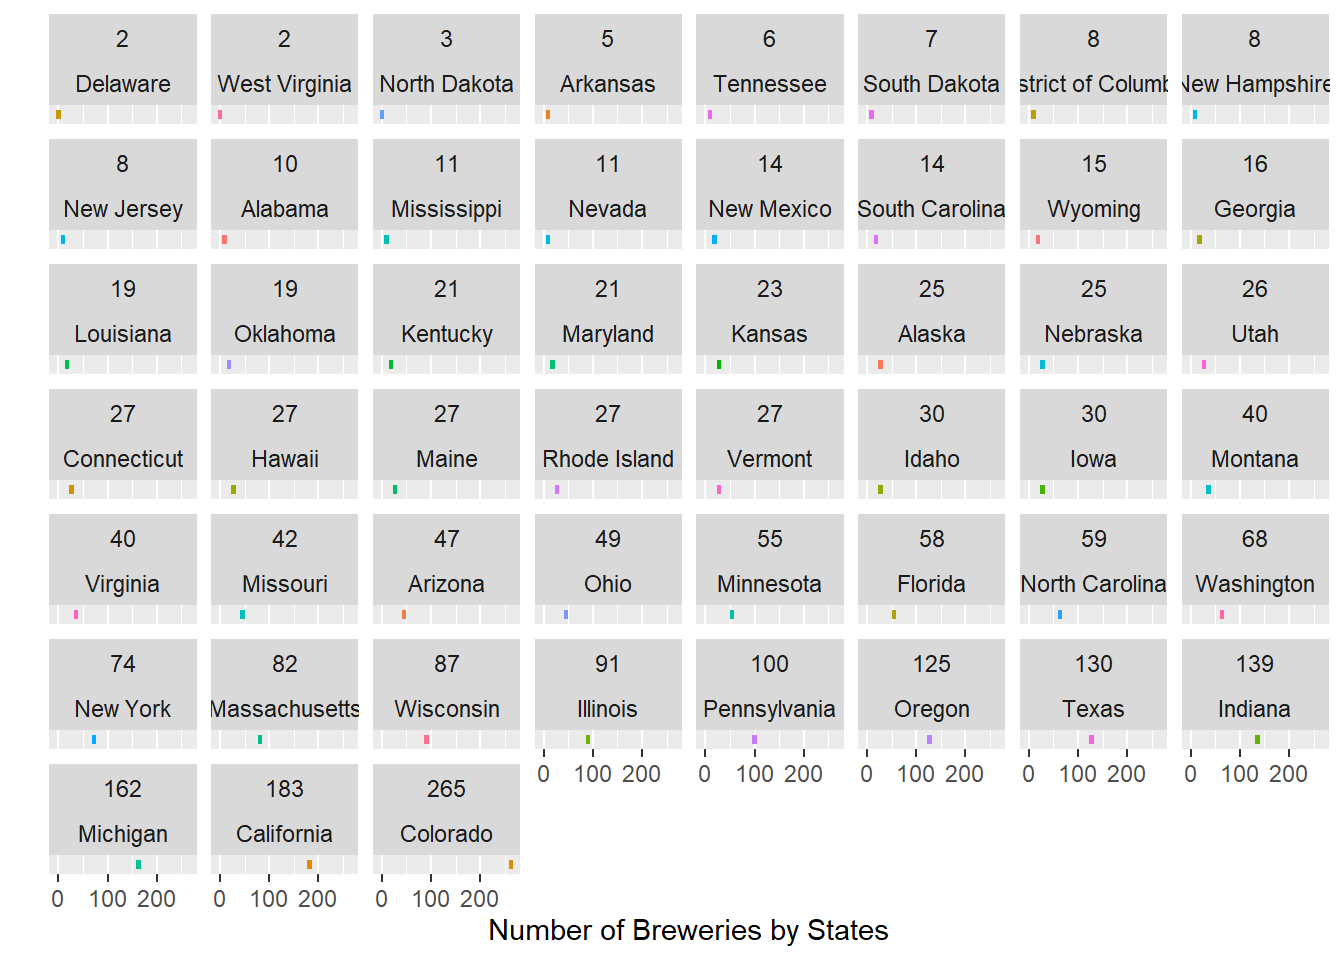
\includegraphics{Employee-Attrition_files/figure-latex/unnamed-chunk-26-1.pdf}

\begin{Shaded}
\begin{Highlighting}[]
\CommentTok{\# Years Since Last Promotion Review \#\#\#\#}
\FunctionTok{filter}\NormalTok{(attrition, JobRole }\SpecialCharTok{==} \StringTok{"Sales Representative"} \SpecialCharTok{|}\NormalTok{ JobRole }\SpecialCharTok{==} \StringTok{"Human Resources"}\NormalTok{) }\SpecialCharTok{\%\textgreater{}\%}
  \FunctionTok{ggplot}\NormalTok{(}\FunctionTok{aes}\NormalTok{(}\AttributeTok{x =}\NormalTok{ YearsSinceLastPromotion, }\AttributeTok{y =}\NormalTok{ JobRole, }\AttributeTok{color =}\NormalTok{ Attrition)) }\SpecialCharTok{+}
  \FunctionTok{geom\_boxplot}\NormalTok{() }\SpecialCharTok{+}
  \FunctionTok{geom\_vline}\NormalTok{(}\FunctionTok{aes}\NormalTok{(}\AttributeTok{xintercept =} \FunctionTok{mean}\NormalTok{(YearsSinceLastPromotion)), }\AttributeTok{color =} \StringTok{"black"}\NormalTok{, }\AttributeTok{linetype =} \StringTok{"dashed"}\NormalTok{) }\SpecialCharTok{+}
  \FunctionTok{ylab}\NormalTok{(}\StringTok{"JobRole"}\NormalTok{) }\SpecialCharTok{+}
  \FunctionTok{xlab}\NormalTok{(}\StringTok{"YearsSinceLastPromotion"}\NormalTok{) }\SpecialCharTok{+}
  \FunctionTok{ggtitle}\NormalTok{(}\StringTok{"Years Since Last Promotion"}\NormalTok{) }\SpecialCharTok{+}
  \FunctionTok{scale\_color\_manual}\NormalTok{(}\AttributeTok{values =}\NormalTok{ colors) }\SpecialCharTok{+}
  \FunctionTok{theme}\NormalTok{(}\AttributeTok{legend.position =} \StringTok{"none"}\NormalTok{) }\SpecialCharTok{+}
  \FunctionTok{theme}\NormalTok{(}\AttributeTok{plot.title =} \FunctionTok{element\_text}\NormalTok{(}\AttributeTok{hjust =} \FloatTok{0.5}\NormalTok{)) }
\end{Highlighting}
\end{Shaded}

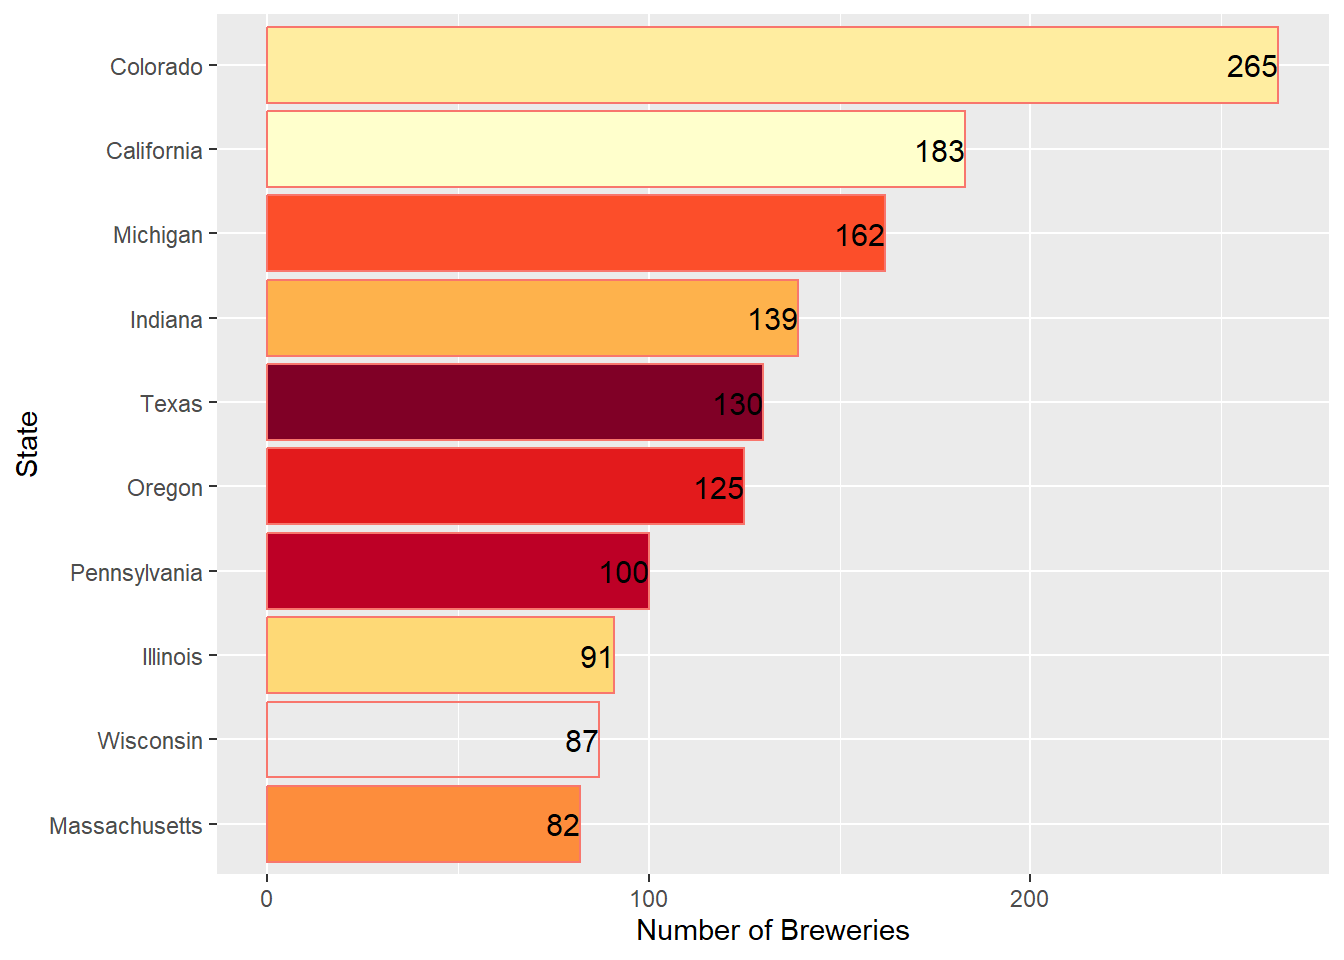
\includegraphics{Employee-Attrition_files/figure-latex/unnamed-chunk-27-1.pdf}

\hypertarget{older-job-role-review}{%
\subsection{Older Job Role Review}\label{older-job-role-review}}

\begin{Shaded}
\begin{Highlighting}[]
\CommentTok{\# JobInvolvement \#\#\#\#}
\FunctionTok{filter}\NormalTok{(attrition, JobRole }\SpecialCharTok{==} \StringTok{"Manager"} \SpecialCharTok{|}\NormalTok{ JobRole }\SpecialCharTok{==} \StringTok{"Research Director"}\NormalTok{ ) }\SpecialCharTok{\%\textgreater{}\%}
  \FunctionTok{ggplot}\NormalTok{(}\FunctionTok{aes}\NormalTok{(}\AttributeTok{x =}\NormalTok{ JobInvolvement, }\AttributeTok{y =}\NormalTok{ JobRole, }\AttributeTok{color =}\NormalTok{ Attrition)) }\SpecialCharTok{+}
  \FunctionTok{geom\_boxplot}\NormalTok{() }\SpecialCharTok{+}
  \FunctionTok{geom\_vline}\NormalTok{(}\FunctionTok{aes}\NormalTok{(}\AttributeTok{xintercept =} \FunctionTok{mean}\NormalTok{(JobInvolvement)), }\AttributeTok{color =} \StringTok{"black"}\NormalTok{, }\AttributeTok{linetype =} \StringTok{"dashed"}\NormalTok{) }\SpecialCharTok{+}
  \FunctionTok{ylab}\NormalTok{(}\StringTok{"JobRole"}\NormalTok{) }\SpecialCharTok{+}
  \FunctionTok{xlab}\NormalTok{(}\StringTok{"JobInvolvement"}\NormalTok{) }\SpecialCharTok{+}
  \FunctionTok{ggtitle}\NormalTok{(}\StringTok{"Job Involvement"}\NormalTok{) }\SpecialCharTok{+}
  \FunctionTok{scale\_color\_manual}\NormalTok{(}\AttributeTok{values =}\NormalTok{ colors) }\SpecialCharTok{+}
  \FunctionTok{theme}\NormalTok{(}\AttributeTok{legend.position =} \StringTok{"none"}\NormalTok{) }\SpecialCharTok{+}
  \FunctionTok{theme}\NormalTok{(}\AttributeTok{plot.title =} \FunctionTok{element\_text}\NormalTok{(}\AttributeTok{hjust =} \FloatTok{0.5}\NormalTok{)) }
\end{Highlighting}
\end{Shaded}

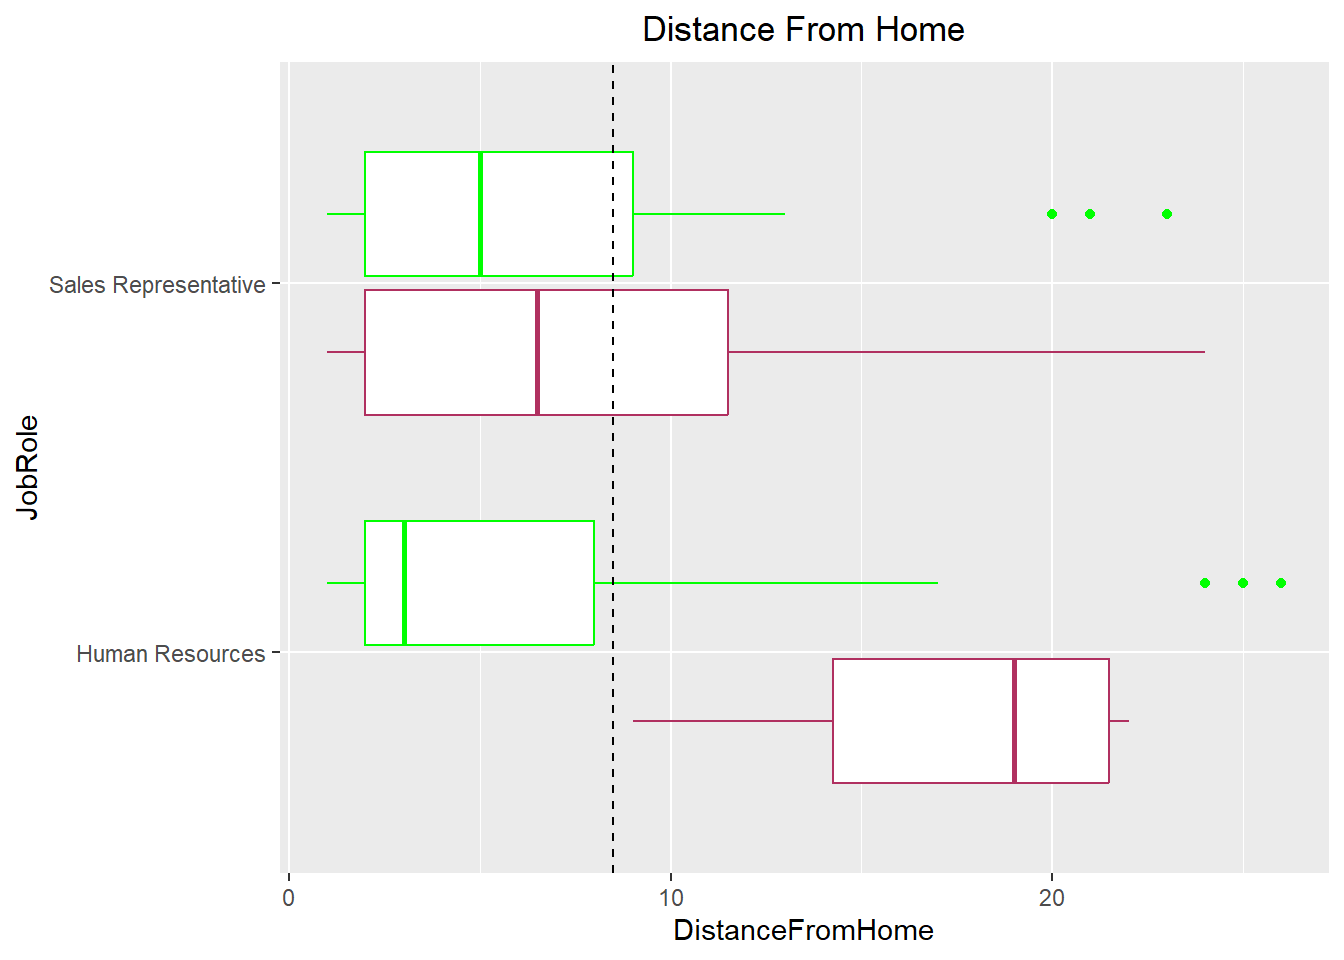
\includegraphics{Employee-Attrition_files/figure-latex/unnamed-chunk-28-1.pdf}

\begin{Shaded}
\begin{Highlighting}[]
\CommentTok{\# RelationshipSatisfaction \#\#\#\#}
\FunctionTok{filter}\NormalTok{(attrition, JobRole }\SpecialCharTok{==} \StringTok{"Manager"} \SpecialCharTok{|}\NormalTok{ JobRole }\SpecialCharTok{==} \StringTok{"Research Director"}\NormalTok{ ) }\SpecialCharTok{\%\textgreater{}\%}
  \FunctionTok{ggplot}\NormalTok{(}\FunctionTok{aes}\NormalTok{(}\AttributeTok{x =}\NormalTok{ RelationshipSatisfaction, }\AttributeTok{y =}\NormalTok{ JobRole, }\AttributeTok{color =}\NormalTok{ Attrition)) }\SpecialCharTok{+}
  \FunctionTok{geom\_boxplot}\NormalTok{() }\SpecialCharTok{+}
  \FunctionTok{geom\_vline}\NormalTok{(}\FunctionTok{aes}\NormalTok{(}\AttributeTok{xintercept =} \FunctionTok{mean}\NormalTok{(RelationshipSatisfaction)), }\AttributeTok{color =} \StringTok{"black"}\NormalTok{, }\AttributeTok{linetype =} \StringTok{"dashed"}\NormalTok{) }\SpecialCharTok{+}
  \FunctionTok{ylab}\NormalTok{(}\StringTok{"JobRole"}\NormalTok{) }\SpecialCharTok{+}
  \FunctionTok{xlab}\NormalTok{(}\StringTok{"RelationshipSatisfaction"}\NormalTok{) }\SpecialCharTok{+}
  \FunctionTok{ggtitle}\NormalTok{(}\StringTok{"Relationship Satisfaction"}\NormalTok{) }\SpecialCharTok{+}
  \FunctionTok{scale\_color\_manual}\NormalTok{(}\AttributeTok{values =}\NormalTok{ colors) }\SpecialCharTok{+}
  \FunctionTok{theme}\NormalTok{(}\AttributeTok{legend.position =} \StringTok{"none"}\NormalTok{) }\SpecialCharTok{+}
  \FunctionTok{theme}\NormalTok{(}\AttributeTok{plot.title =} \FunctionTok{element\_text}\NormalTok{(}\AttributeTok{hjust =} \FloatTok{0.5}\NormalTok{)) }
\end{Highlighting}
\end{Shaded}

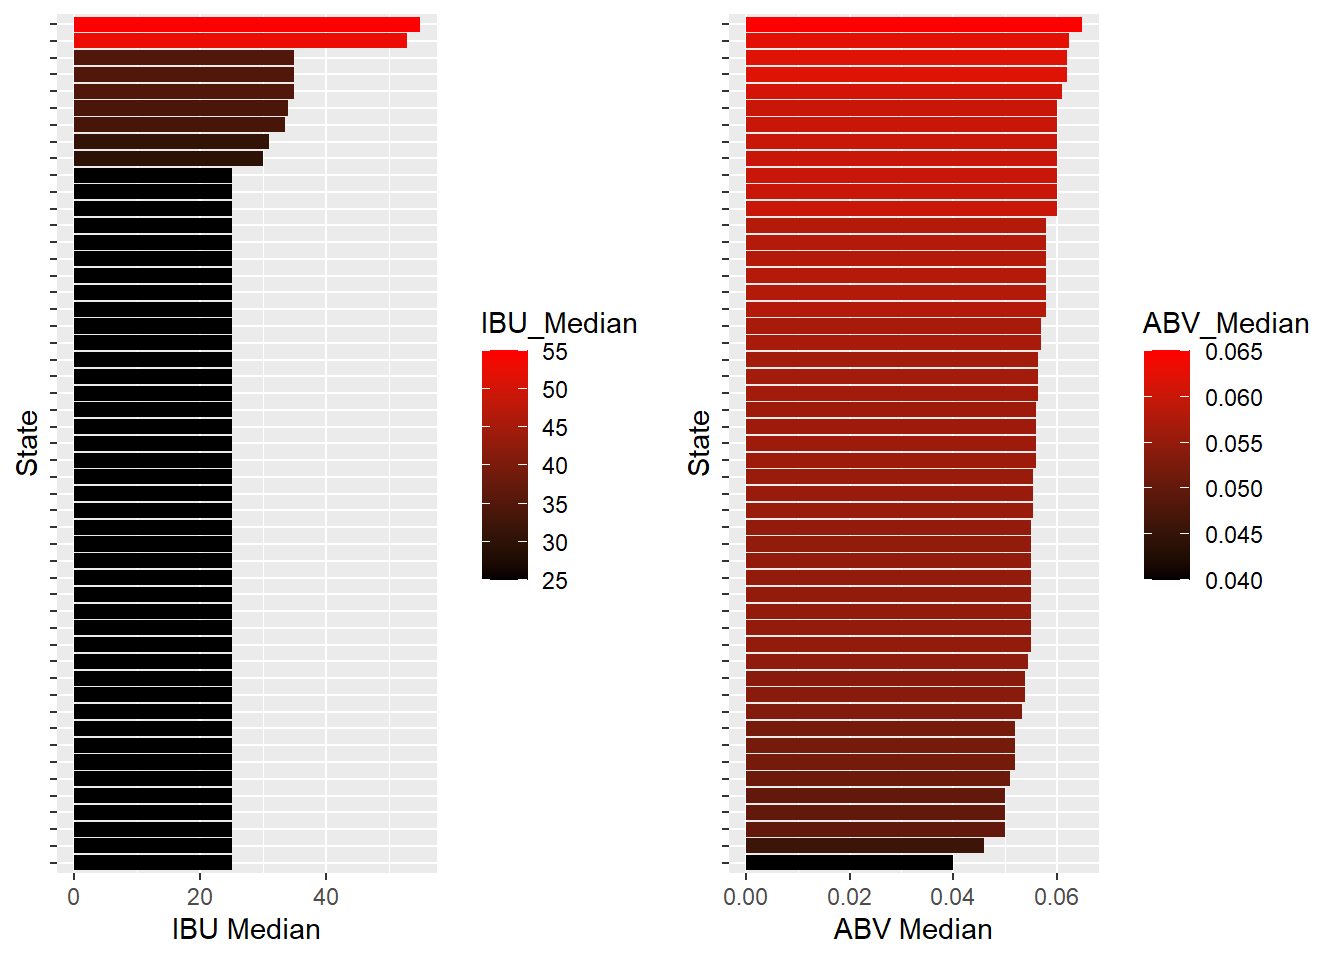
\includegraphics{Employee-Attrition_files/figure-latex/unnamed-chunk-29-1.pdf}

\begin{Shaded}
\begin{Highlighting}[]
\CommentTok{\# Total Working Years \#\#\#\#}
\FunctionTok{filter}\NormalTok{(attrition, JobRole }\SpecialCharTok{==} \StringTok{"Manager"} \SpecialCharTok{|}\NormalTok{ JobRole }\SpecialCharTok{==} \StringTok{"Research Director"}\NormalTok{ ) }\SpecialCharTok{\%\textgreater{}\%}
  \FunctionTok{ggplot}\NormalTok{(}\FunctionTok{aes}\NormalTok{(}\AttributeTok{x =}\NormalTok{ TotalWorkingYears, }\AttributeTok{y =}\NormalTok{ JobRole, }\AttributeTok{color =}\NormalTok{ Attrition)) }\SpecialCharTok{+}
  \FunctionTok{geom\_boxplot}\NormalTok{() }\SpecialCharTok{+}
  \FunctionTok{geom\_vline}\NormalTok{(}\FunctionTok{aes}\NormalTok{(}\AttributeTok{xintercept =} \FunctionTok{mean}\NormalTok{(TotalWorkingYears)), }\AttributeTok{color =} \StringTok{"black"}\NormalTok{, }\AttributeTok{linetype =} \StringTok{"dashed"}\NormalTok{) }\SpecialCharTok{+}
  \FunctionTok{ylab}\NormalTok{(}\StringTok{"JobRole"}\NormalTok{) }\SpecialCharTok{+}
  \FunctionTok{xlab}\NormalTok{(}\StringTok{"TotalWorkingYears"}\NormalTok{) }\SpecialCharTok{+}
  \FunctionTok{ggtitle}\NormalTok{(}\StringTok{"Total Working Years"}\NormalTok{) }\SpecialCharTok{+}
  \FunctionTok{scale\_color\_manual}\NormalTok{(}\AttributeTok{values =}\NormalTok{ colors) }\SpecialCharTok{+}
  \FunctionTok{theme}\NormalTok{(}\AttributeTok{legend.position =} \StringTok{"none"}\NormalTok{) }\SpecialCharTok{+}
  \FunctionTok{theme}\NormalTok{(}\AttributeTok{plot.title =} \FunctionTok{element\_text}\NormalTok{(}\AttributeTok{hjust =} \FloatTok{0.5}\NormalTok{)) }
\end{Highlighting}
\end{Shaded}

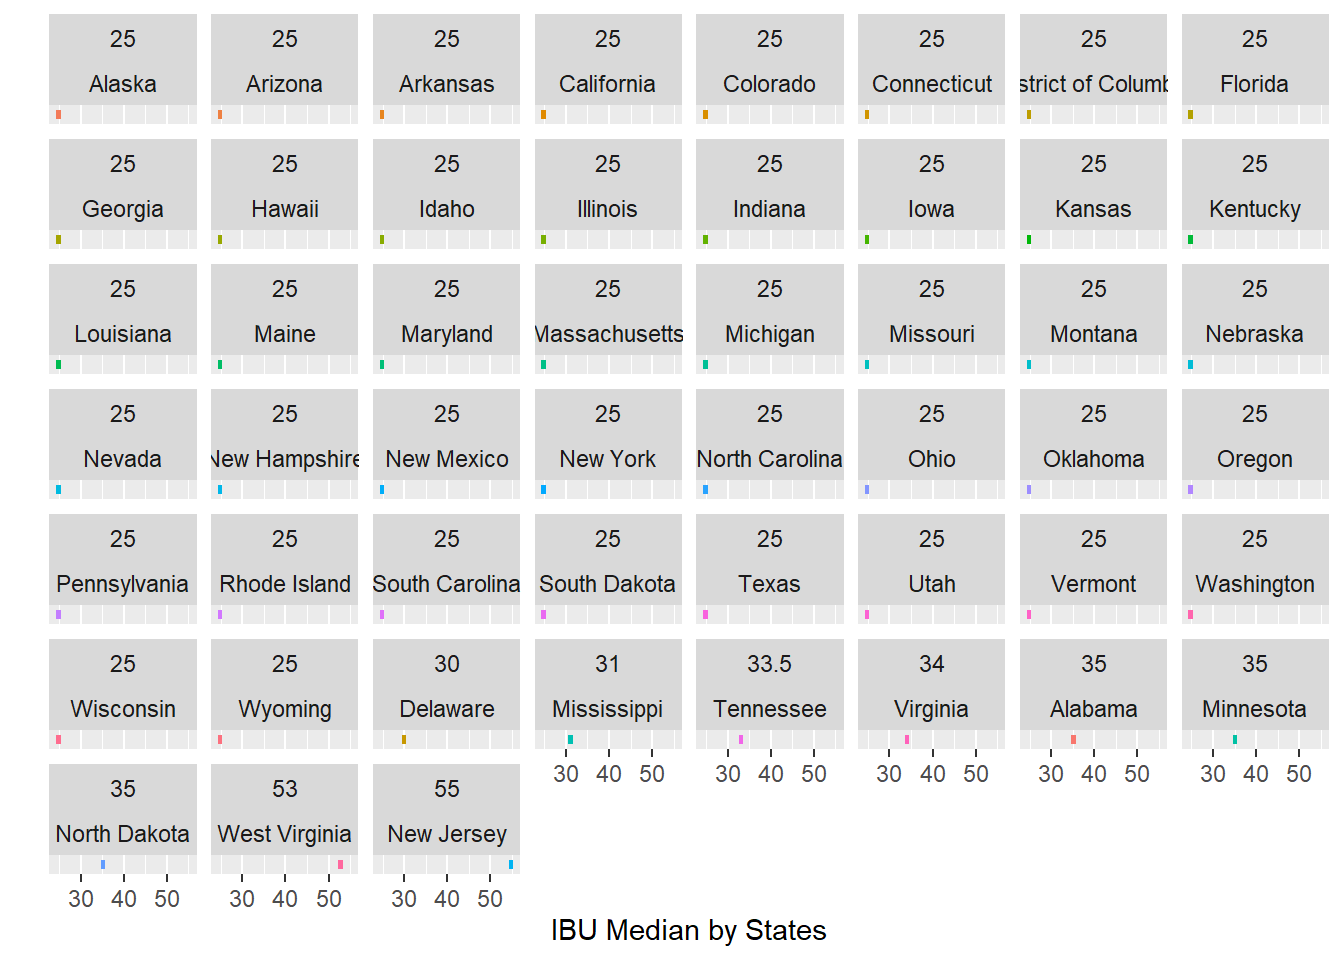
\includegraphics{Employee-Attrition_files/figure-latex/unnamed-chunk-30-1.pdf}

\begin{Shaded}
\begin{Highlighting}[]
\CommentTok{\# Education \#\#\#\#}
\FunctionTok{filter}\NormalTok{(attrition, JobRole }\SpecialCharTok{==} \StringTok{"Manager"} \SpecialCharTok{|}\NormalTok{ JobRole }\SpecialCharTok{==} \StringTok{"Research Director"}\NormalTok{ ) }\SpecialCharTok{\%\textgreater{}\%}
  \FunctionTok{ggplot}\NormalTok{(}\FunctionTok{aes}\NormalTok{(}\AttributeTok{x =}\NormalTok{ Education, }\AttributeTok{y =}\NormalTok{ JobRole, }\AttributeTok{color =}\NormalTok{ Attrition)) }\SpecialCharTok{+}
  \FunctionTok{geom\_boxplot}\NormalTok{() }\SpecialCharTok{+}
  \FunctionTok{geom\_vline}\NormalTok{(}\FunctionTok{aes}\NormalTok{(}\AttributeTok{xintercept =} \FunctionTok{mean}\NormalTok{(Education)), }\AttributeTok{color =} \StringTok{"black"}\NormalTok{, }\AttributeTok{linetype =} \StringTok{"dashed"}\NormalTok{) }\SpecialCharTok{+}
  \FunctionTok{ylab}\NormalTok{(}\StringTok{"JobRole"}\NormalTok{) }\SpecialCharTok{+}
  \FunctionTok{xlab}\NormalTok{(}\StringTok{"Education"}\NormalTok{) }\SpecialCharTok{+}
  \FunctionTok{ggtitle}\NormalTok{(}\StringTok{"Education"}\NormalTok{) }\SpecialCharTok{+}
  \FunctionTok{scale\_color\_manual}\NormalTok{(}\AttributeTok{values =}\NormalTok{ colors) }\SpecialCharTok{+}
  \FunctionTok{theme}\NormalTok{(}\AttributeTok{legend.position =} \StringTok{"none"}\NormalTok{) }\SpecialCharTok{+}
  \FunctionTok{theme}\NormalTok{(}\AttributeTok{plot.title =} \FunctionTok{element\_text}\NormalTok{(}\AttributeTok{hjust =} \FloatTok{0.5}\NormalTok{)) }
\end{Highlighting}
\end{Shaded}

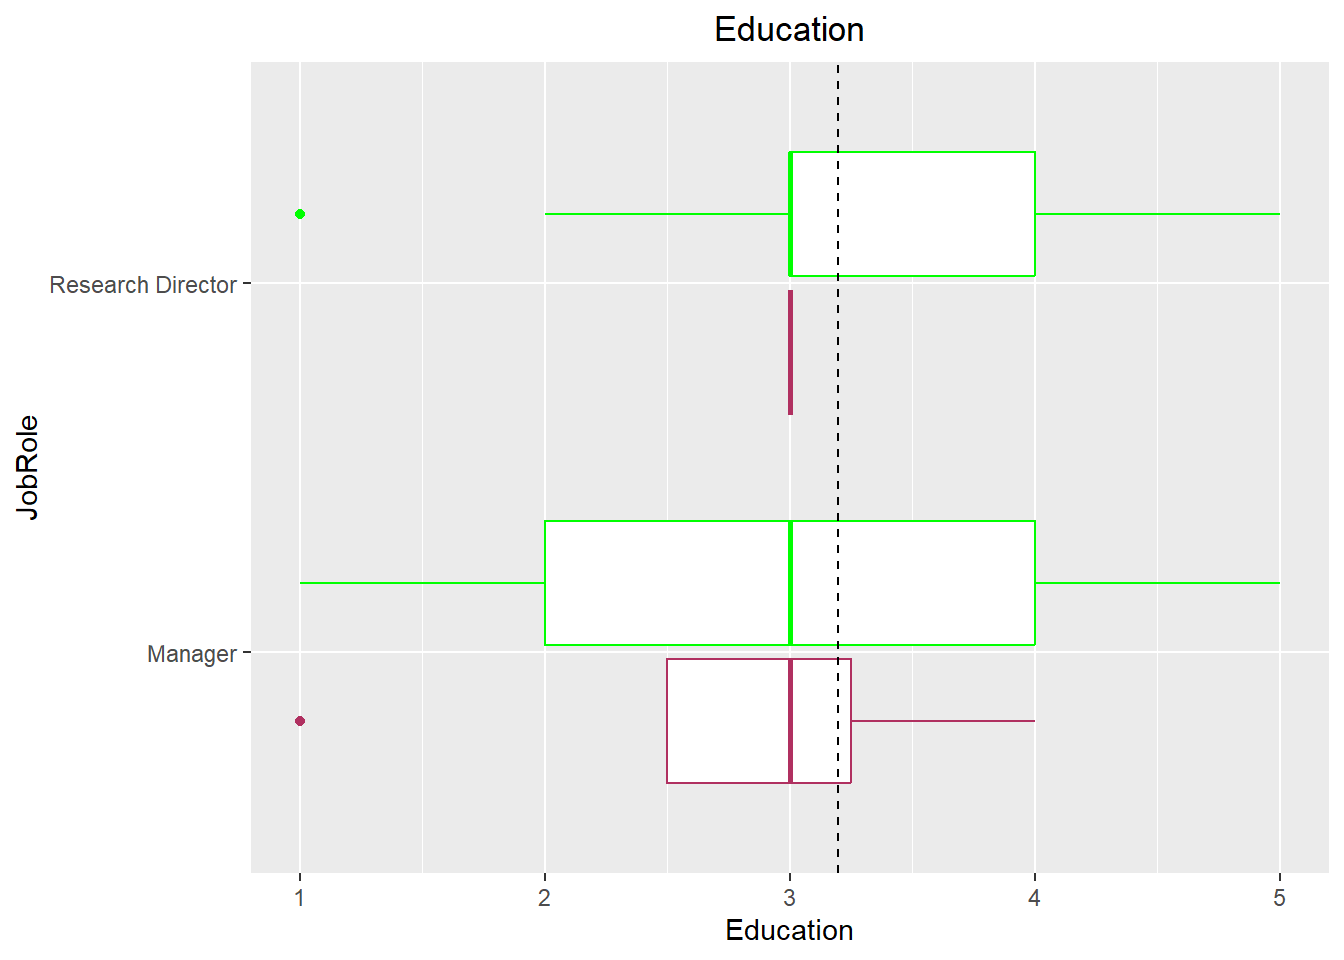
\includegraphics{Employee-Attrition_files/figure-latex/unnamed-chunk-31-1.pdf}

\begin{Shaded}
\begin{Highlighting}[]
\CommentTok{\# Years in Current Role \#\#\#\#}
\FunctionTok{filter}\NormalTok{(attrition, JobRole }\SpecialCharTok{==} \StringTok{"Manager"} \SpecialCharTok{|}\NormalTok{ JobRole }\SpecialCharTok{==} \StringTok{"Research Director"}\NormalTok{ ) }\SpecialCharTok{\%\textgreater{}\%}
  \FunctionTok{ggplot}\NormalTok{(}\FunctionTok{aes}\NormalTok{(}\AttributeTok{x =}\NormalTok{ YearsInCurrentRole, }\AttributeTok{y =}\NormalTok{ JobRole, }\AttributeTok{color =}\NormalTok{ Attrition)) }\SpecialCharTok{+}
  \FunctionTok{geom\_boxplot}\NormalTok{() }\SpecialCharTok{+}
  \FunctionTok{geom\_vline}\NormalTok{(}\FunctionTok{aes}\NormalTok{(}\AttributeTok{xintercept =} \FunctionTok{mean}\NormalTok{(YearsInCurrentRole)), }\AttributeTok{color =} \StringTok{"black"}\NormalTok{, }\AttributeTok{linetype =} \StringTok{"dashed"}\NormalTok{) }\SpecialCharTok{+}
  \FunctionTok{ylab}\NormalTok{(}\StringTok{"JobRole"}\NormalTok{) }\SpecialCharTok{+}
  \FunctionTok{xlab}\NormalTok{(}\StringTok{"YearsInCurrentRole"}\NormalTok{) }\SpecialCharTok{+}
  \FunctionTok{ggtitle}\NormalTok{(}\StringTok{"Years In Current Role"}\NormalTok{) }\SpecialCharTok{+}
  \FunctionTok{scale\_color\_manual}\NormalTok{(}\AttributeTok{values =}\NormalTok{ colors) }\SpecialCharTok{+}
  \FunctionTok{theme}\NormalTok{(}\AttributeTok{legend.position =} \StringTok{"none"}\NormalTok{) }\SpecialCharTok{+}
  \FunctionTok{theme}\NormalTok{(}\AttributeTok{plot.title =} \FunctionTok{element\_text}\NormalTok{(}\AttributeTok{hjust =} \FloatTok{0.5}\NormalTok{)) }
\end{Highlighting}
\end{Shaded}

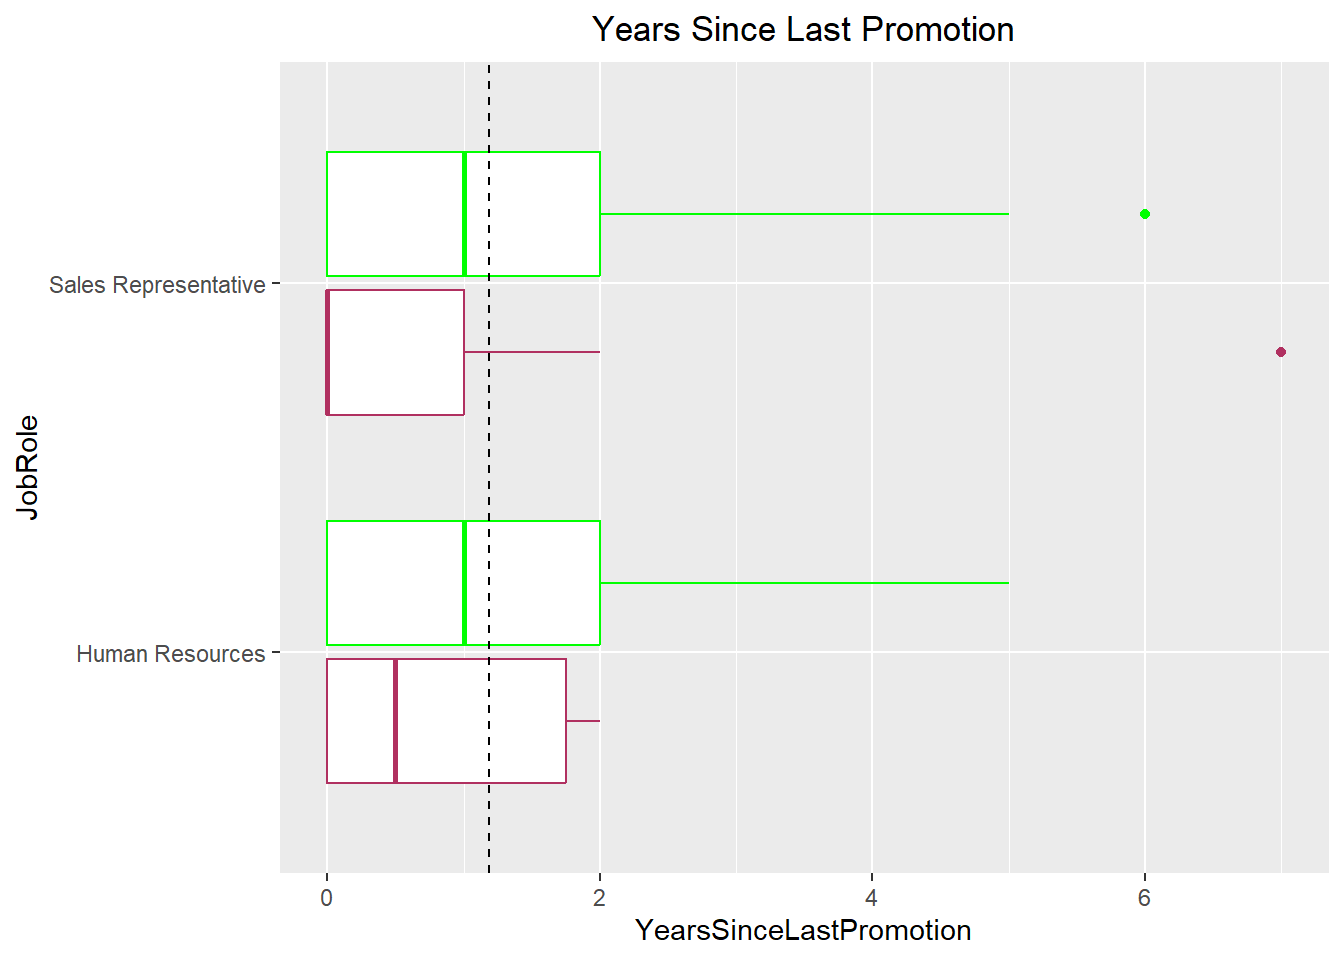
\includegraphics{Employee-Attrition_files/figure-latex/unnamed-chunk-32-1.pdf}

\begin{Shaded}
\begin{Highlighting}[]
\CommentTok{\# Years Since Last Promotion Review \#\#\#\#}
\FunctionTok{filter}\NormalTok{(attrition, JobRole }\SpecialCharTok{==} \StringTok{"Manager"} \SpecialCharTok{|}\NormalTok{ JobRole }\SpecialCharTok{==} \StringTok{"Research Director"}\NormalTok{ ) }\SpecialCharTok{\%\textgreater{}\%}
  \FunctionTok{ggplot}\NormalTok{(}\FunctionTok{aes}\NormalTok{(}\AttributeTok{x =}\NormalTok{ YearsSinceLastPromotion, }\AttributeTok{y =}\NormalTok{ JobRole, }\AttributeTok{color =}\NormalTok{ Attrition)) }\SpecialCharTok{+}
  \FunctionTok{geom\_boxplot}\NormalTok{() }\SpecialCharTok{+}
  \FunctionTok{geom\_vline}\NormalTok{(}\FunctionTok{aes}\NormalTok{(}\AttributeTok{xintercept =} \FunctionTok{mean}\NormalTok{(YearsSinceLastPromotion)), }\AttributeTok{color =} \StringTok{"black"}\NormalTok{, }\AttributeTok{linetype =} \StringTok{"dashed"}\NormalTok{) }\SpecialCharTok{+}
  \FunctionTok{ylab}\NormalTok{(}\StringTok{"JobRole"}\NormalTok{) }\SpecialCharTok{+}
  \FunctionTok{xlab}\NormalTok{(}\StringTok{"YearsSinceLastPromotion"}\NormalTok{) }\SpecialCharTok{+}
  \FunctionTok{ggtitle}\NormalTok{(}\StringTok{"Years Since Last Promotion"}\NormalTok{) }\SpecialCharTok{+}
  \FunctionTok{scale\_color\_manual}\NormalTok{(}\AttributeTok{values =}\NormalTok{ colors) }\SpecialCharTok{+}
  \FunctionTok{theme}\NormalTok{(}\AttributeTok{legend.position =} \StringTok{"none"}\NormalTok{) }\SpecialCharTok{+}
  \FunctionTok{theme}\NormalTok{(}\AttributeTok{plot.title =} \FunctionTok{element\_text}\NormalTok{(}\AttributeTok{hjust =} \FloatTok{0.5}\NormalTok{)) }
\end{Highlighting}
\end{Shaded}

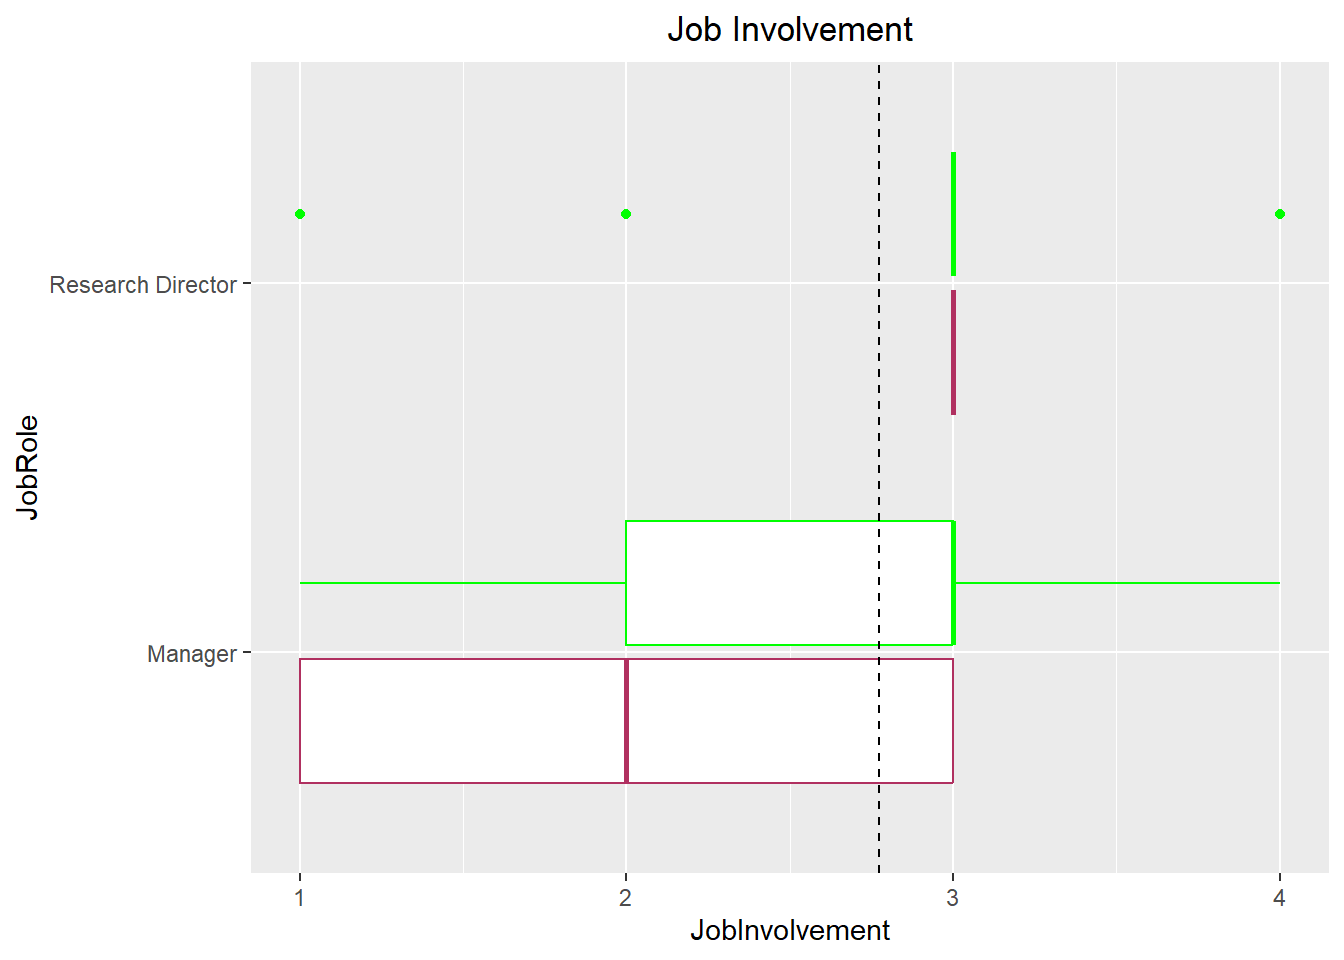
\includegraphics{Employee-Attrition_files/figure-latex/unnamed-chunk-33-1.pdf}

\hypertarget{generation-z-specific}{%
\subsection{Generation z Specific}\label{generation-z-specific}}

\begin{Shaded}
\begin{Highlighting}[]
\CommentTok{\# Training Times Last Year \#\#\#\#}
\NormalTok{t }\OtherTok{\textless{}{-}} \FunctionTok{filter}\NormalTok{(attrition, JobRole }\SpecialCharTok{==} \StringTok{"Sales Representative"} \SpecialCharTok{|}\NormalTok{ JobRole }\SpecialCharTok{==} \StringTok{"Human Resources"} \SpecialCharTok{\&}\NormalTok{ Age }\SpecialCharTok{\textless{}} \DecValTok{22}\NormalTok{) }\SpecialCharTok{\%\textgreater{}\%}
  \FunctionTok{ggplot}\NormalTok{(}\FunctionTok{aes}\NormalTok{(}\AttributeTok{x =}\NormalTok{ TrainingTimesLastYear, }\AttributeTok{y =}\NormalTok{ JobRole, }\AttributeTok{color =}\NormalTok{ Attrition)) }\SpecialCharTok{+}
  \FunctionTok{geom\_boxplot}\NormalTok{() }\SpecialCharTok{+}
  \FunctionTok{geom\_vline}\NormalTok{(}\FunctionTok{aes}\NormalTok{(}\AttributeTok{xintercept =} \FunctionTok{mean}\NormalTok{(TrainingTimesLastYear)), }\AttributeTok{color =} \StringTok{"black"}\NormalTok{, }\AttributeTok{linetype =} \StringTok{"dashed"}\NormalTok{) }\SpecialCharTok{+}
  \FunctionTok{ylab}\NormalTok{(}\StringTok{"JobRole"}\NormalTok{) }\SpecialCharTok{+}
  \FunctionTok{xlab}\NormalTok{(}\StringTok{"TrainingTimesLastYear"}\NormalTok{) }\SpecialCharTok{+}
  \FunctionTok{ggtitle}\NormalTok{(}\StringTok{"Training Times Last Year"}\NormalTok{) }\SpecialCharTok{+}
  \FunctionTok{scale\_color\_manual}\NormalTok{(}\AttributeTok{values =}\NormalTok{ colors) }\SpecialCharTok{+}
  \FunctionTok{theme}\NormalTok{(}\AttributeTok{legend.position =} \StringTok{"none"}\NormalTok{) }\SpecialCharTok{+}
  \FunctionTok{theme}\NormalTok{(}\AttributeTok{plot.title =} \FunctionTok{element\_text}\NormalTok{(}\AttributeTok{hjust =} \FloatTok{0.5}\NormalTok{)) }


\CommentTok{\# Education \#\#\#\#}
\NormalTok{e }\OtherTok{\textless{}{-}} \FunctionTok{filter}\NormalTok{(attrition, JobRole }\SpecialCharTok{==} \StringTok{"Sales Representative"} \SpecialCharTok{|}\NormalTok{ JobRole }\SpecialCharTok{==} \StringTok{"Human Resources"} \SpecialCharTok{\&}\NormalTok{ Age }\SpecialCharTok{\textless{}} \DecValTok{22}\NormalTok{) }\SpecialCharTok{\%\textgreater{}\%}
  \FunctionTok{ggplot}\NormalTok{(}\FunctionTok{aes}\NormalTok{(}\AttributeTok{x =}\NormalTok{ Education, }\AttributeTok{y =}\NormalTok{ JobRole, }\AttributeTok{color =}\NormalTok{ Attrition)) }\SpecialCharTok{+}
  \FunctionTok{geom\_boxplot}\NormalTok{() }\SpecialCharTok{+}
  \FunctionTok{geom\_vline}\NormalTok{(}\FunctionTok{aes}\NormalTok{(}\AttributeTok{xintercept =} \FunctionTok{mean}\NormalTok{(Education)), }\AttributeTok{color =} \StringTok{"black"}\NormalTok{, }\AttributeTok{linetype =} \StringTok{"dashed"}\NormalTok{) }\SpecialCharTok{+}
  \FunctionTok{ylab}\NormalTok{(}\StringTok{"JobRole"}\NormalTok{) }\SpecialCharTok{+}
  \FunctionTok{xlab}\NormalTok{(}\StringTok{"Education"}\NormalTok{) }\SpecialCharTok{+}
  \FunctionTok{ggtitle}\NormalTok{(}\StringTok{"Education"}\NormalTok{) }\SpecialCharTok{+}
  \FunctionTok{scale\_color\_manual}\NormalTok{(}\AttributeTok{values =}\NormalTok{ colors) }\SpecialCharTok{+}
  \FunctionTok{theme}\NormalTok{(}\AttributeTok{legend.position =} \StringTok{"none"}\NormalTok{) }\SpecialCharTok{+}
  \FunctionTok{theme}\NormalTok{(}\AttributeTok{plot.title =} \FunctionTok{element\_text}\NormalTok{(}\AttributeTok{hjust =} \FloatTok{0.5}\NormalTok{)) }


\FunctionTok{grid.arrange}\NormalTok{(t, e, }\AttributeTok{nrow =} \DecValTok{2}\NormalTok{)}
\end{Highlighting}
\end{Shaded}

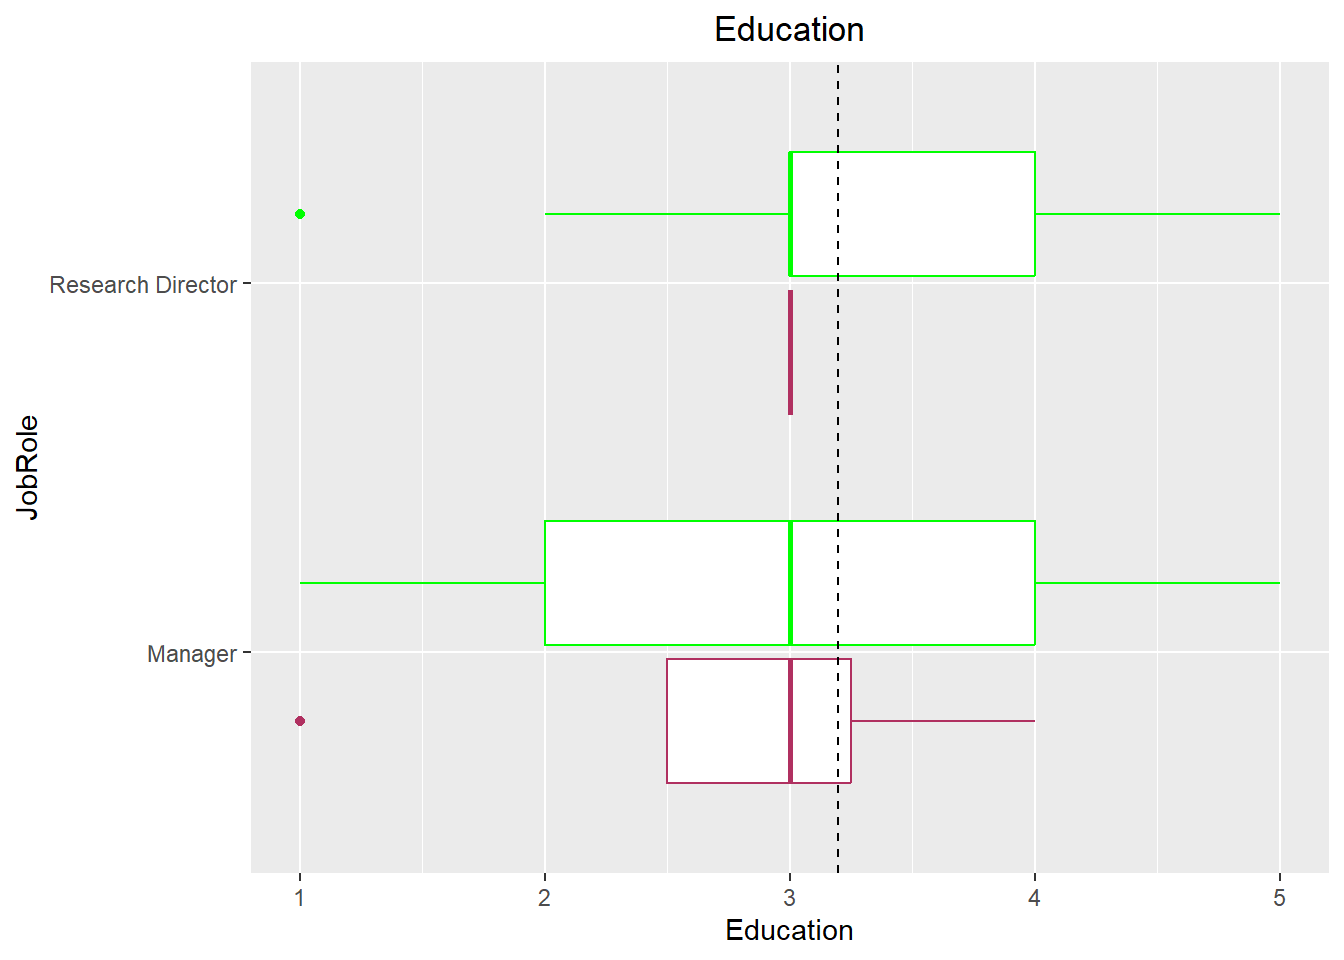
\includegraphics{Employee-Attrition_files/figure-latex/unnamed-chunk-34-1.pdf}

\begin{Shaded}
\begin{Highlighting}[]
\CommentTok{\# Distance From Home \#\#\#\#}
\FunctionTok{filter}\NormalTok{(attrition, JobRole }\SpecialCharTok{==} \StringTok{"Sales Representative"} \SpecialCharTok{|}\NormalTok{ JobRole }\SpecialCharTok{==} \StringTok{"Human Resources"} \SpecialCharTok{\&}\NormalTok{ Age }\SpecialCharTok{\textless{}} \DecValTok{22}\NormalTok{) }\SpecialCharTok{\%\textgreater{}\%}
  \FunctionTok{ggplot}\NormalTok{(}\FunctionTok{aes}\NormalTok{(}\AttributeTok{x =}\NormalTok{ DistanceFromHome, }\AttributeTok{y =}\NormalTok{ JobRole, }\AttributeTok{color =}\NormalTok{ Attrition)) }\SpecialCharTok{+}
  \FunctionTok{geom\_boxplot}\NormalTok{() }\SpecialCharTok{+}
  \FunctionTok{geom\_vline}\NormalTok{(}\FunctionTok{aes}\NormalTok{(}\AttributeTok{xintercept =} \FunctionTok{mean}\NormalTok{(DistanceFromHome)), }\AttributeTok{color =} \StringTok{"black"}\NormalTok{, }\AttributeTok{linetype =} \StringTok{"dashed"}\NormalTok{) }\SpecialCharTok{+}
  \FunctionTok{ylab}\NormalTok{(}\StringTok{"JobRole"}\NormalTok{) }\SpecialCharTok{+}
  \FunctionTok{xlab}\NormalTok{(}\StringTok{"DistanceFromHome"}\NormalTok{) }\SpecialCharTok{+}
  \FunctionTok{ggtitle}\NormalTok{(}\StringTok{"Distance From Home"}\NormalTok{) }\SpecialCharTok{+}
  \FunctionTok{scale\_color\_manual}\NormalTok{(}\AttributeTok{values =}\NormalTok{ colors) }\SpecialCharTok{+}
  \FunctionTok{theme}\NormalTok{(}\AttributeTok{legend.position =} \StringTok{"none"}\NormalTok{) }\SpecialCharTok{+}
  \FunctionTok{theme}\NormalTok{(}\AttributeTok{plot.title =} \FunctionTok{element\_text}\NormalTok{(}\AttributeTok{hjust =} \FloatTok{0.5}\NormalTok{)) }
\end{Highlighting}
\end{Shaded}

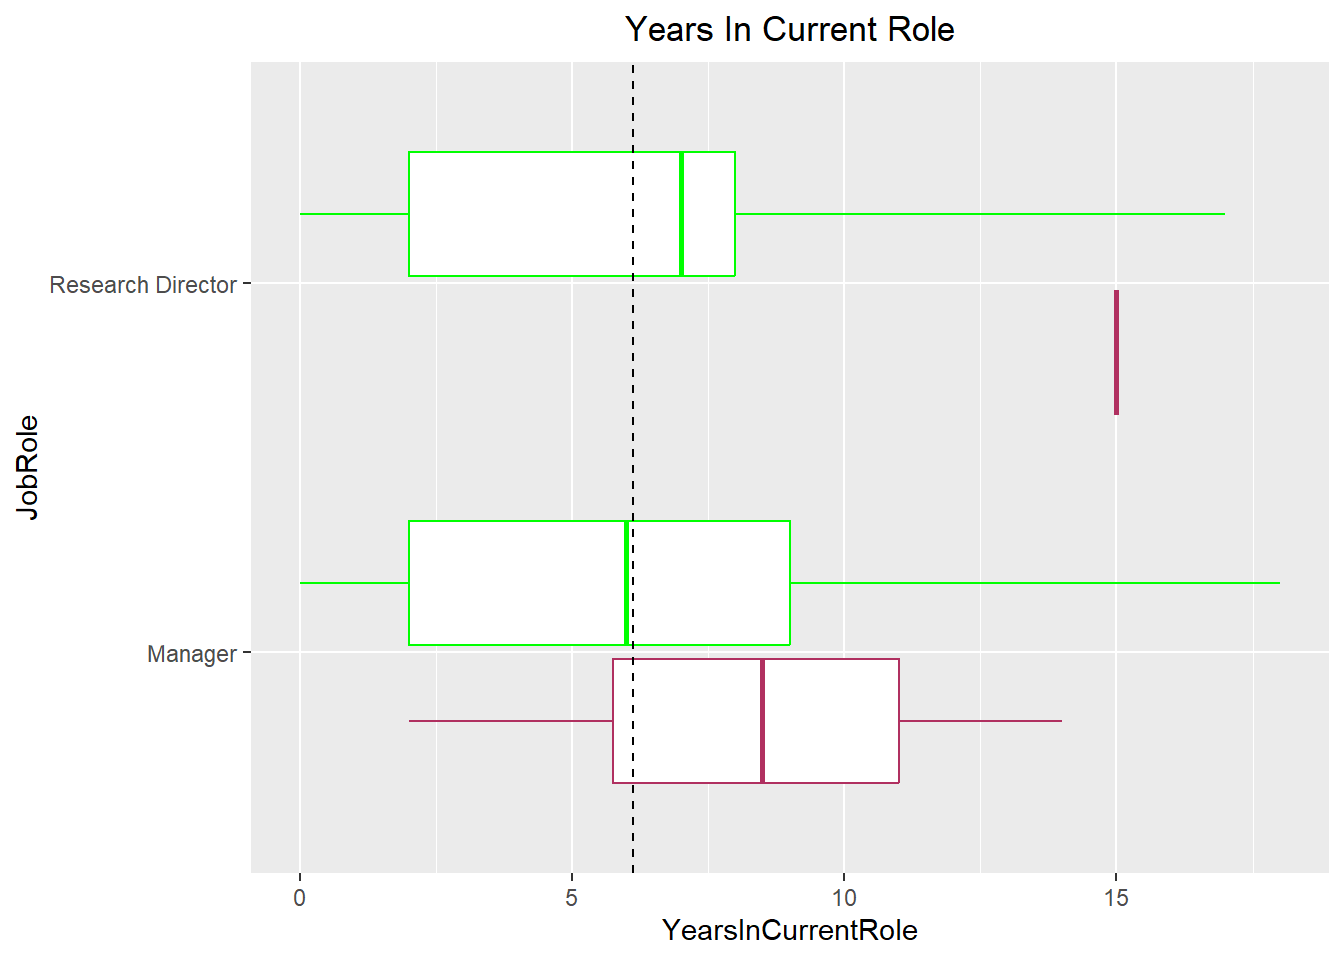
\includegraphics{Employee-Attrition_files/figure-latex/unnamed-chunk-35-1.pdf}

\begin{Shaded}
\begin{Highlighting}[]
\CommentTok{\# Years in Current Role \#\#\#\#}
\NormalTok{y }\OtherTok{\textless{}{-}} \FunctionTok{filter}\NormalTok{(attrition, JobRole }\SpecialCharTok{==} \StringTok{"Sales Representative"} \SpecialCharTok{|}\NormalTok{ JobRole }\SpecialCharTok{==} \StringTok{"Human Resources"} \SpecialCharTok{\&}\NormalTok{ Age }\SpecialCharTok{\textless{}} \DecValTok{22}\NormalTok{) }\SpecialCharTok{\%\textgreater{}\%}
  \FunctionTok{ggplot}\NormalTok{(}\FunctionTok{aes}\NormalTok{(}\AttributeTok{x =}\NormalTok{ YearsInCurrentRole, }\AttributeTok{y =}\NormalTok{ JobRole, }\AttributeTok{color =}\NormalTok{ Attrition)) }\SpecialCharTok{+}
  \FunctionTok{geom\_boxplot}\NormalTok{() }\SpecialCharTok{+}
  \FunctionTok{geom\_vline}\NormalTok{(}\FunctionTok{aes}\NormalTok{(}\AttributeTok{xintercept =} \FunctionTok{mean}\NormalTok{(YearsInCurrentRole)), }\AttributeTok{color =} \StringTok{"black"}\NormalTok{, }\AttributeTok{linetype =} \StringTok{"dashed"}\NormalTok{) }\SpecialCharTok{+}
  \FunctionTok{ylab}\NormalTok{(}\StringTok{"JobRole"}\NormalTok{) }\SpecialCharTok{+}
  \FunctionTok{xlab}\NormalTok{(}\StringTok{"YearsInCurrentRole"}\NormalTok{) }\SpecialCharTok{+}
  \FunctionTok{ggtitle}\NormalTok{(}\StringTok{"Years In Current Role"}\NormalTok{) }\SpecialCharTok{+}
  \FunctionTok{scale\_color\_manual}\NormalTok{(}\AttributeTok{values =}\NormalTok{ colors) }\SpecialCharTok{+}
  \FunctionTok{theme}\NormalTok{(}\AttributeTok{legend.position =} \StringTok{"none"}\NormalTok{) }\SpecialCharTok{+}
  \FunctionTok{theme}\NormalTok{(}\AttributeTok{plot.title =} \FunctionTok{element\_text}\NormalTok{(}\AttributeTok{hjust =} \FloatTok{0.5}\NormalTok{)) }

\CommentTok{\# Years Since Last Promotion Review \#\#\#\#}
\NormalTok{p }\OtherTok{\textless{}{-}} \FunctionTok{filter}\NormalTok{(attrition, JobRole }\SpecialCharTok{==} \StringTok{"Sales Representative"} \SpecialCharTok{|}\NormalTok{ JobRole }\SpecialCharTok{==} \StringTok{"Human Resources"} \SpecialCharTok{\&}\NormalTok{ Age }\SpecialCharTok{\textless{}} \DecValTok{22}\NormalTok{) }\SpecialCharTok{\%\textgreater{}\%}
  \FunctionTok{ggplot}\NormalTok{(}\FunctionTok{aes}\NormalTok{(}\AttributeTok{x =}\NormalTok{ YearsSinceLastPromotion, }\AttributeTok{y =}\NormalTok{ JobRole, }\AttributeTok{color =}\NormalTok{ Attrition)) }\SpecialCharTok{+}
  \FunctionTok{geom\_boxplot}\NormalTok{() }\SpecialCharTok{+}
  \FunctionTok{geom\_vline}\NormalTok{(}\FunctionTok{aes}\NormalTok{(}\AttributeTok{xintercept =} \FunctionTok{mean}\NormalTok{(YearsSinceLastPromotion)), }\AttributeTok{color =} \StringTok{"black"}\NormalTok{, }\AttributeTok{linetype =} \StringTok{"dashed"}\NormalTok{) }\SpecialCharTok{+}
  \FunctionTok{ylab}\NormalTok{(}\StringTok{"JobRole"}\NormalTok{) }\SpecialCharTok{+}
  \FunctionTok{xlab}\NormalTok{(}\StringTok{"YearsSinceLastPromotion"}\NormalTok{) }\SpecialCharTok{+}
  \FunctionTok{ggtitle}\NormalTok{(}\StringTok{"Years Since Last Promotion"}\NormalTok{) }\SpecialCharTok{+}
  \FunctionTok{scale\_color\_manual}\NormalTok{(}\AttributeTok{values =}\NormalTok{ colors) }\SpecialCharTok{+}
  \FunctionTok{theme}\NormalTok{(}\AttributeTok{legend.position =} \StringTok{"none"}\NormalTok{) }\SpecialCharTok{+}
  \FunctionTok{theme}\NormalTok{(}\AttributeTok{plot.title =} \FunctionTok{element\_text}\NormalTok{(}\AttributeTok{hjust =} \FloatTok{0.5}\NormalTok{)) }


\FunctionTok{grid.arrange}\NormalTok{(y, p, }\AttributeTok{nrow =} \DecValTok{2}\NormalTok{)}
\end{Highlighting}
\end{Shaded}

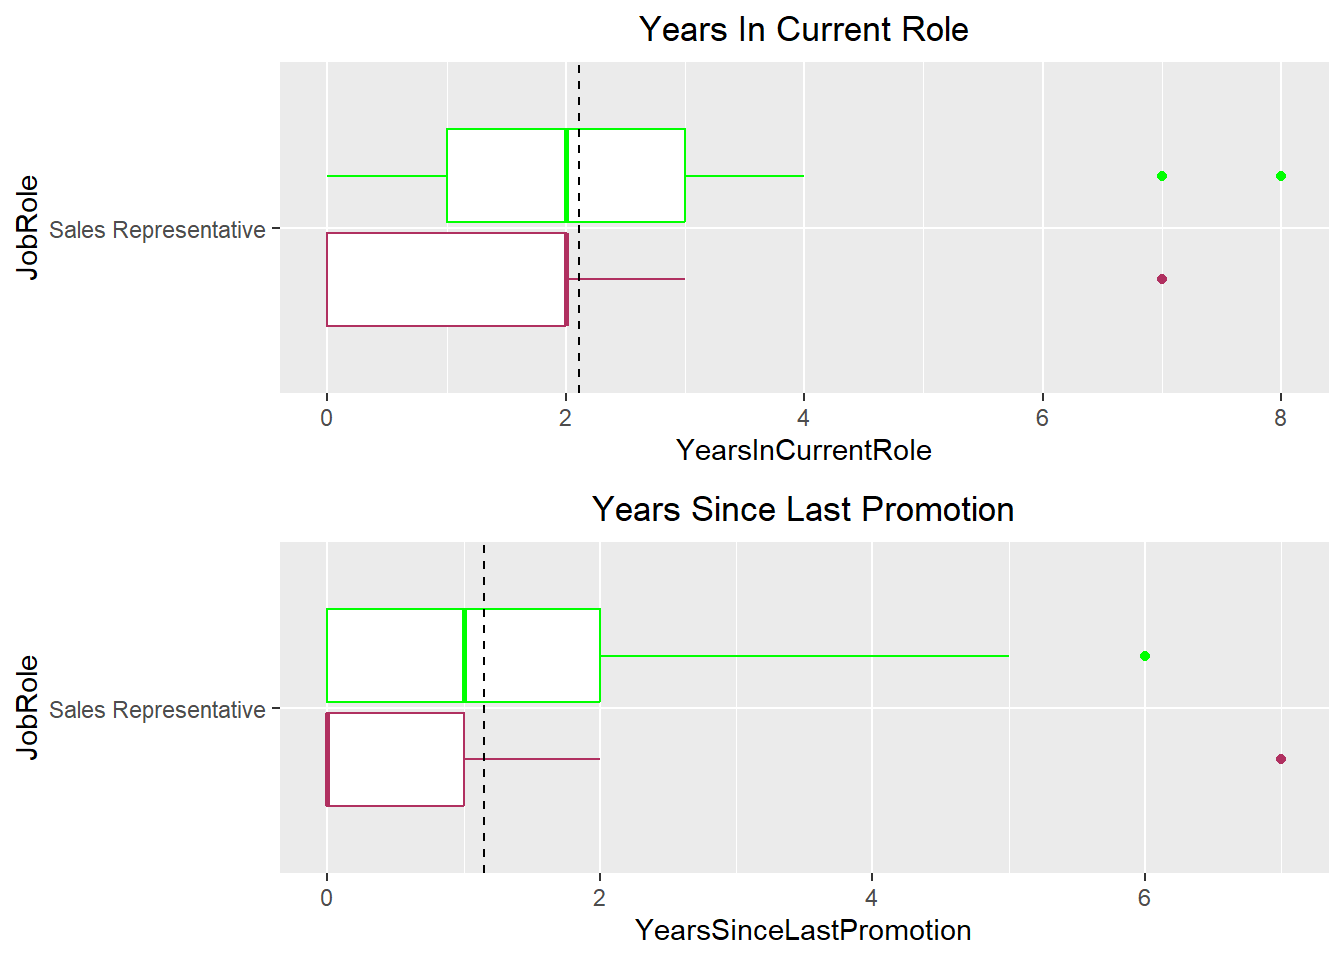
\includegraphics{Employee-Attrition_files/figure-latex/unnamed-chunk-36-1.pdf}

\hypertarget{all-aged-groups}{%
\subsection{All Aged Groups}\label{all-aged-groups}}

\begin{Shaded}
\begin{Highlighting}[]
\CommentTok{\# Training Times Last Year \#\#\#\#}
\NormalTok{t }\OtherTok{\textless{}{-}} \FunctionTok{filter}\NormalTok{(attrition, JobRole }\SpecialCharTok{==} \StringTok{"Research Scientist"} \SpecialCharTok{|}\NormalTok{ JobRole }\SpecialCharTok{==} \StringTok{"Sales Executive"}  \SpecialCharTok{|}\NormalTok{ JobRole }\SpecialCharTok{==} \StringTok{"Laboratory Technician"} \SpecialCharTok{|}\NormalTok{ JobRole }\SpecialCharTok{==} \StringTok{"Healthcare Representative"}\SpecialCharTok{|}\NormalTok{ JobRole }\SpecialCharTok{==} \StringTok{"Manufacturing Director"}\NormalTok{ ) }\SpecialCharTok{\%\textgreater{}\%}
  \FunctionTok{ggplot}\NormalTok{(}\FunctionTok{aes}\NormalTok{(}\AttributeTok{x =}\NormalTok{ TrainingTimesLastYear, }\AttributeTok{y =}\NormalTok{ JobRole, }\AttributeTok{color =}\NormalTok{ Attrition)) }\SpecialCharTok{+}
  \FunctionTok{geom\_boxplot}\NormalTok{() }\SpecialCharTok{+}
  \FunctionTok{geom\_vline}\NormalTok{(}\FunctionTok{aes}\NormalTok{(}\AttributeTok{xintercept =} \FunctionTok{mean}\NormalTok{(TrainingTimesLastYear)), }\AttributeTok{color =} \StringTok{"black"}\NormalTok{, }\AttributeTok{linetype =} \StringTok{"dashed"}\NormalTok{) }\SpecialCharTok{+}
  \FunctionTok{ylab}\NormalTok{(}\StringTok{"JobRole"}\NormalTok{) }\SpecialCharTok{+}
  \FunctionTok{xlab}\NormalTok{(}\StringTok{"TrainingTimesLastYear"}\NormalTok{) }\SpecialCharTok{+}
  \FunctionTok{ggtitle}\NormalTok{(}\StringTok{"Training Times Last Year"}\NormalTok{) }\SpecialCharTok{+}
  \FunctionTok{scale\_color\_manual}\NormalTok{(}\AttributeTok{values =}\NormalTok{ colors) }\SpecialCharTok{+}
  \FunctionTok{theme}\NormalTok{(}\AttributeTok{legend.position =} \StringTok{"none"}\NormalTok{) }\SpecialCharTok{+}
  \FunctionTok{theme}\NormalTok{(}\AttributeTok{plot.title =} \FunctionTok{element\_text}\NormalTok{(}\AttributeTok{hjust =} \FloatTok{0.5}\NormalTok{)) }


\CommentTok{\# Education \#\#\#\#}
\NormalTok{e }\OtherTok{\textless{}{-}} \FunctionTok{filter}\NormalTok{(attrition, JobRole }\SpecialCharTok{==} \StringTok{"Research Scientist"} \SpecialCharTok{|}\NormalTok{ JobRole }\SpecialCharTok{==} \StringTok{"Sales Executive"}  \SpecialCharTok{|}\NormalTok{ JobRole }\SpecialCharTok{==} \StringTok{"Laboratory Technician"} \SpecialCharTok{|}\NormalTok{ JobRole }\SpecialCharTok{==} \StringTok{"Healthcare Representative"}\SpecialCharTok{|}\NormalTok{ JobRole }\SpecialCharTok{==} \StringTok{"Manufacturing Director"}\NormalTok{ ) }\SpecialCharTok{\%\textgreater{}\%}
  \FunctionTok{ggplot}\NormalTok{(}\FunctionTok{aes}\NormalTok{(}\AttributeTok{x =}\NormalTok{ Education, }\AttributeTok{y =}\NormalTok{ JobRole, }\AttributeTok{color =}\NormalTok{ Attrition)) }\SpecialCharTok{+}
  \FunctionTok{geom\_boxplot}\NormalTok{() }\SpecialCharTok{+}
  \FunctionTok{geom\_vline}\NormalTok{(}\FunctionTok{aes}\NormalTok{(}\AttributeTok{xintercept =} \FunctionTok{mean}\NormalTok{(Education)), }\AttributeTok{color =} \StringTok{"black"}\NormalTok{, }\AttributeTok{linetype =} \StringTok{"dashed"}\NormalTok{) }\SpecialCharTok{+}
  \FunctionTok{ylab}\NormalTok{(}\StringTok{"JobRole"}\NormalTok{) }\SpecialCharTok{+}
  \FunctionTok{xlab}\NormalTok{(}\StringTok{"Education"}\NormalTok{) }\SpecialCharTok{+}
  \FunctionTok{ggtitle}\NormalTok{(}\StringTok{"Education"}\NormalTok{) }\SpecialCharTok{+}
  \FunctionTok{scale\_color\_manual}\NormalTok{(}\AttributeTok{values =}\NormalTok{ colors) }\SpecialCharTok{+}
  \FunctionTok{theme}\NormalTok{(}\AttributeTok{legend.position =} \StringTok{"none"}\NormalTok{) }\SpecialCharTok{+}
  \FunctionTok{theme}\NormalTok{(}\AttributeTok{plot.title =} \FunctionTok{element\_text}\NormalTok{(}\AttributeTok{hjust =} \FloatTok{0.5}\NormalTok{)) }


\FunctionTok{grid.arrange}\NormalTok{(t, e, }\AttributeTok{nrow =} \DecValTok{2}\NormalTok{)}
\end{Highlighting}
\end{Shaded}

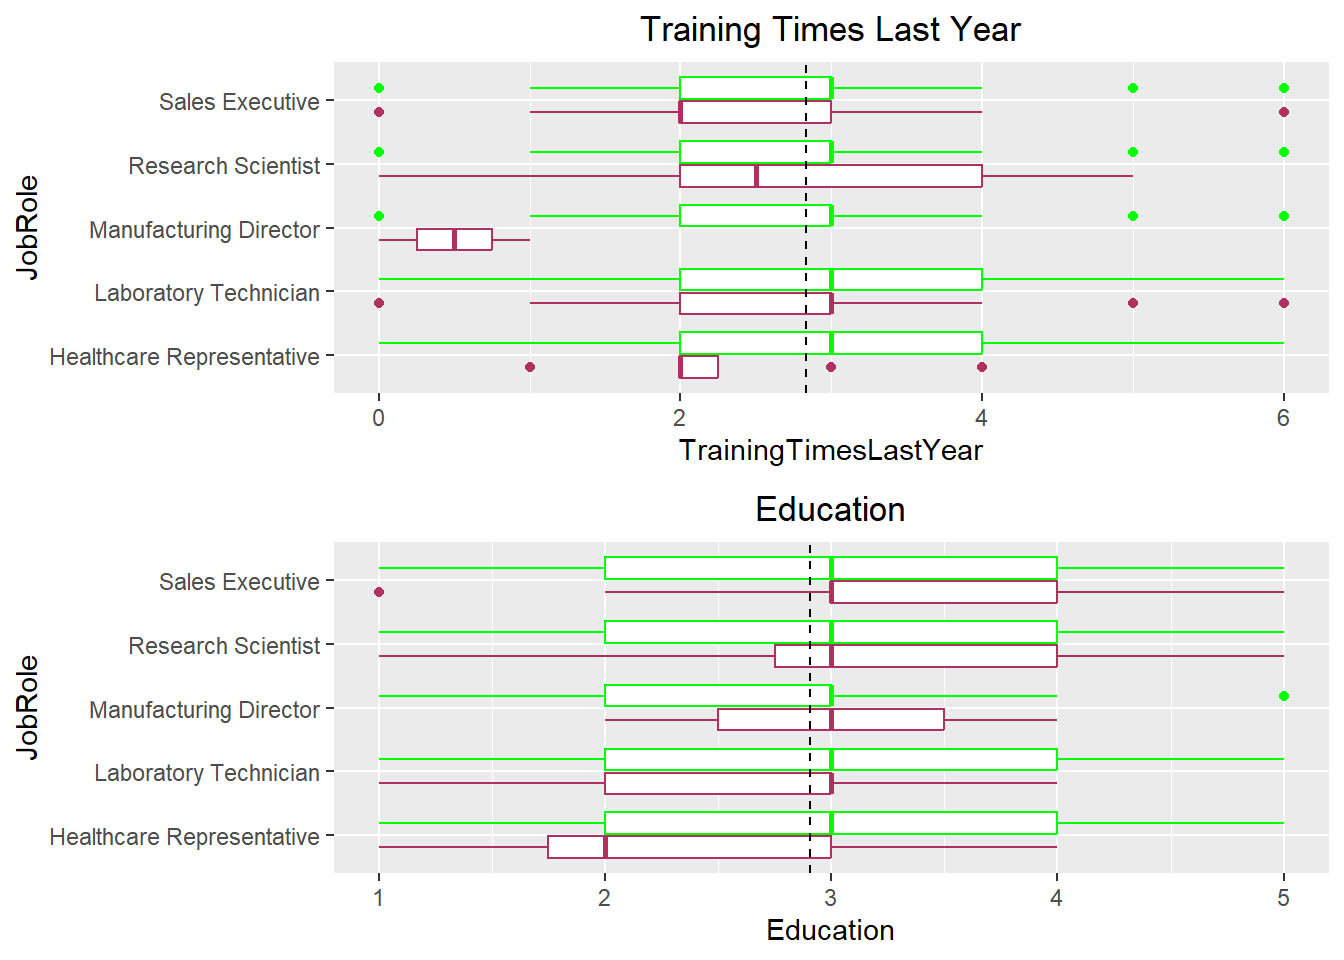
\includegraphics{Employee-Attrition_files/figure-latex/unnamed-chunk-37-1.pdf}

\begin{Shaded}
\begin{Highlighting}[]
\CommentTok{\# Distance From Home \#\#\#\#}
\FunctionTok{filter}\NormalTok{(attrition, JobRole }\SpecialCharTok{==} \StringTok{"Research Scientist"} \SpecialCharTok{|}\NormalTok{ JobRole }\SpecialCharTok{==} \StringTok{"Sales Executive"}  \SpecialCharTok{|}\NormalTok{ JobRole }\SpecialCharTok{==} \StringTok{"Laboratory Technician"} \SpecialCharTok{|}\NormalTok{ JobRole }\SpecialCharTok{==} \StringTok{"Healthcare Representative"}\SpecialCharTok{|}\NormalTok{ JobRole }\SpecialCharTok{==} \StringTok{"Manufacturing Director"}\NormalTok{ ) }\SpecialCharTok{\%\textgreater{}\%}
  \FunctionTok{ggplot}\NormalTok{(}\FunctionTok{aes}\NormalTok{(}\AttributeTok{x =}\NormalTok{ DistanceFromHome, }\AttributeTok{y =}\NormalTok{ JobRole, }\AttributeTok{color =}\NormalTok{ Attrition)) }\SpecialCharTok{+}
  \FunctionTok{geom\_boxplot}\NormalTok{() }\SpecialCharTok{+}
  \FunctionTok{geom\_vline}\NormalTok{(}\FunctionTok{aes}\NormalTok{(}\AttributeTok{xintercept =} \FunctionTok{mean}\NormalTok{(DistanceFromHome)), }\AttributeTok{color =} \StringTok{"black"}\NormalTok{, }\AttributeTok{linetype =} \StringTok{"dashed"}\NormalTok{) }\SpecialCharTok{+}
  \FunctionTok{ylab}\NormalTok{(}\StringTok{"JobRole"}\NormalTok{) }\SpecialCharTok{+}
  \FunctionTok{xlab}\NormalTok{(}\StringTok{"DistanceFromHome"}\NormalTok{) }\SpecialCharTok{+}
  \FunctionTok{ggtitle}\NormalTok{(}\StringTok{"Distance From Home"}\NormalTok{) }\SpecialCharTok{+}
  \FunctionTok{scale\_color\_manual}\NormalTok{(}\AttributeTok{values =}\NormalTok{ colors) }\SpecialCharTok{+}
  \FunctionTok{theme}\NormalTok{(}\AttributeTok{legend.position =} \StringTok{"none"}\NormalTok{) }\SpecialCharTok{+}
  \FunctionTok{theme}\NormalTok{(}\AttributeTok{plot.title =} \FunctionTok{element\_text}\NormalTok{(}\AttributeTok{hjust =} \FloatTok{0.5}\NormalTok{)) }
\end{Highlighting}
\end{Shaded}

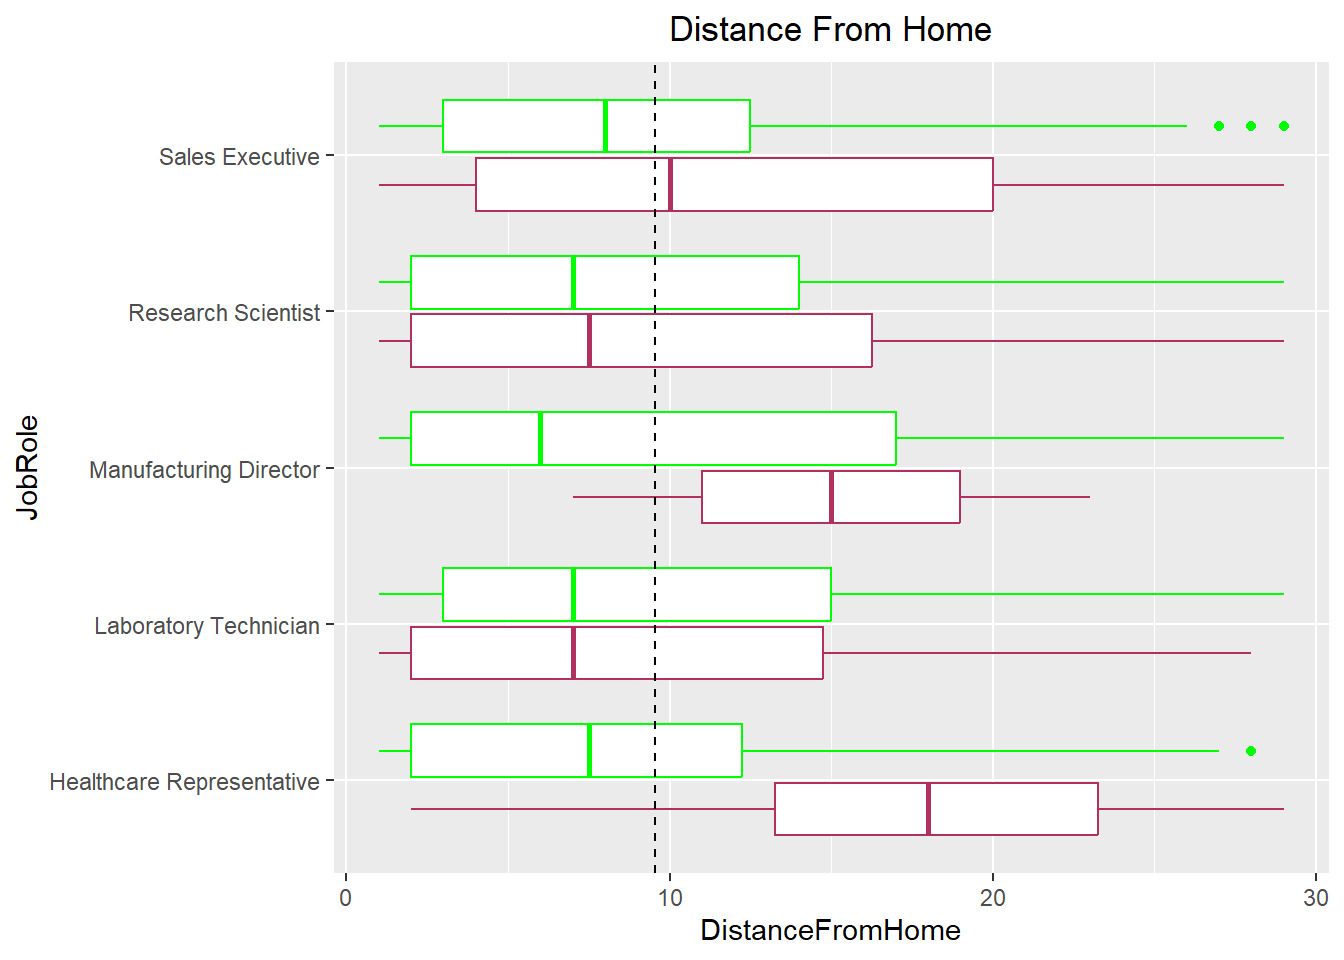
\includegraphics{Employee-Attrition_files/figure-latex/unnamed-chunk-38-1.pdf}

\begin{Shaded}
\begin{Highlighting}[]
\CommentTok{\# Years in Current Role \#\#\#\#}
\NormalTok{y }\OtherTok{\textless{}{-}} \FunctionTok{filter}\NormalTok{(attrition, JobRole }\SpecialCharTok{==} \StringTok{"Research Scientist"} \SpecialCharTok{|}\NormalTok{ JobRole }\SpecialCharTok{==} \StringTok{"Sales Executive"}  \SpecialCharTok{|}\NormalTok{ JobRole }\SpecialCharTok{==} \StringTok{"Laboratory Technician"} \SpecialCharTok{|}\NormalTok{ JobRole }\SpecialCharTok{==} \StringTok{"Healthcare Representative"}\SpecialCharTok{|}\NormalTok{ JobRole }\SpecialCharTok{==} \StringTok{"Manufacturing Director"}\NormalTok{ ) }\SpecialCharTok{\%\textgreater{}\%}
  \FunctionTok{ggplot}\NormalTok{(}\FunctionTok{aes}\NormalTok{(}\AttributeTok{x =}\NormalTok{ YearsInCurrentRole, }\AttributeTok{y =}\NormalTok{ JobRole, }\AttributeTok{color =}\NormalTok{ Attrition)) }\SpecialCharTok{+}
  \FunctionTok{geom\_boxplot}\NormalTok{() }\SpecialCharTok{+}
  \FunctionTok{geom\_vline}\NormalTok{(}\FunctionTok{aes}\NormalTok{(}\AttributeTok{xintercept =} \FunctionTok{mean}\NormalTok{(YearsInCurrentRole)), }\AttributeTok{color =} \StringTok{"black"}\NormalTok{, }\AttributeTok{linetype =} \StringTok{"dashed"}\NormalTok{) }\SpecialCharTok{+}
  \FunctionTok{ylab}\NormalTok{(}\StringTok{"JobRole"}\NormalTok{) }\SpecialCharTok{+}
  \FunctionTok{xlab}\NormalTok{(}\StringTok{"YearsInCurrentRole"}\NormalTok{) }\SpecialCharTok{+}
  \FunctionTok{ggtitle}\NormalTok{(}\StringTok{"Years In Current Role"}\NormalTok{) }\SpecialCharTok{+}
  \FunctionTok{scale\_color\_manual}\NormalTok{(}\AttributeTok{values =}\NormalTok{ colors) }\SpecialCharTok{+}
  \FunctionTok{theme}\NormalTok{(}\AttributeTok{legend.position =} \StringTok{"none"}\NormalTok{) }\SpecialCharTok{+}
  \FunctionTok{theme}\NormalTok{(}\AttributeTok{plot.title =} \FunctionTok{element\_text}\NormalTok{(}\AttributeTok{hjust =} \FloatTok{0.5}\NormalTok{)) }

\CommentTok{\# Years Since Last Promotion Review \#\#\#\#}
\NormalTok{p }\OtherTok{\textless{}{-}} \FunctionTok{filter}\NormalTok{(attrition, JobRole }\SpecialCharTok{==} \StringTok{"Research Scientist"} \SpecialCharTok{|}\NormalTok{ JobRole }\SpecialCharTok{==} \StringTok{"Sales Executive"}  \SpecialCharTok{|}\NormalTok{ JobRole }\SpecialCharTok{==} \StringTok{"Laboratory Technician"} \SpecialCharTok{|}\NormalTok{ JobRole }\SpecialCharTok{==} \StringTok{"Healthcare Representative"}\SpecialCharTok{|}\NormalTok{ JobRole }\SpecialCharTok{==} \StringTok{"Manufacturing Director"}\NormalTok{ ) }\SpecialCharTok{\%\textgreater{}\%}
  \FunctionTok{ggplot}\NormalTok{(}\FunctionTok{aes}\NormalTok{(}\AttributeTok{x =}\NormalTok{ YearsSinceLastPromotion, }\AttributeTok{y =}\NormalTok{ JobRole, }\AttributeTok{color =}\NormalTok{ Attrition)) }\SpecialCharTok{+}
  \FunctionTok{geom\_boxplot}\NormalTok{() }\SpecialCharTok{+}
  \FunctionTok{geom\_vline}\NormalTok{(}\FunctionTok{aes}\NormalTok{(}\AttributeTok{xintercept =} \FunctionTok{mean}\NormalTok{(YearsSinceLastPromotion)), }\AttributeTok{color =} \StringTok{"black"}\NormalTok{, }\AttributeTok{linetype =} \StringTok{"dashed"}\NormalTok{) }\SpecialCharTok{+}
  \FunctionTok{ylab}\NormalTok{(}\StringTok{"JobRole"}\NormalTok{) }\SpecialCharTok{+}
  \FunctionTok{xlab}\NormalTok{(}\StringTok{"YearsSinceLastPromotion"}\NormalTok{) }\SpecialCharTok{+}
  \FunctionTok{ggtitle}\NormalTok{(}\StringTok{"Years Since Last Promotion"}\NormalTok{) }\SpecialCharTok{+}
  \FunctionTok{scale\_color\_manual}\NormalTok{(}\AttributeTok{values =}\NormalTok{ colors) }\SpecialCharTok{+}
  \FunctionTok{theme}\NormalTok{(}\AttributeTok{legend.position =} \StringTok{"none"}\NormalTok{) }\SpecialCharTok{+}
  \FunctionTok{theme}\NormalTok{(}\AttributeTok{plot.title =} \FunctionTok{element\_text}\NormalTok{(}\AttributeTok{hjust =} \FloatTok{0.5}\NormalTok{)) }


\FunctionTok{grid.arrange}\NormalTok{(y, p, }\AttributeTok{nrow =} \DecValTok{2}\NormalTok{)}
\end{Highlighting}
\end{Shaded}

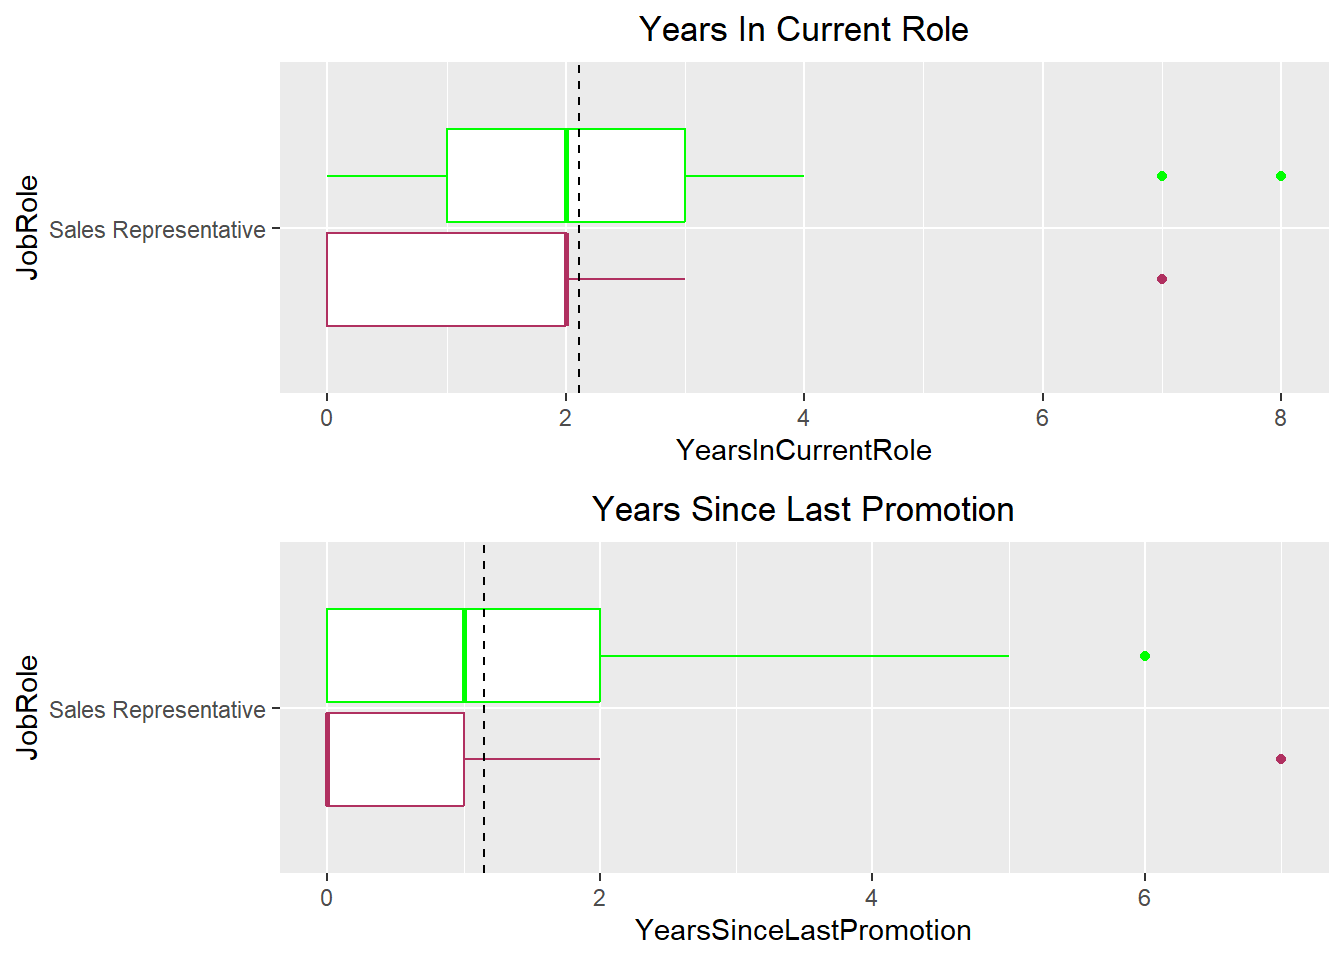
\includegraphics{Employee-Attrition_files/figure-latex/unnamed-chunk-39-1.pdf}

\hypertarget{knn---k-nearest-neighbors}{%
\subsection{KNN - K Nearest Neighbors}\label{knn---k-nearest-neighbors}}

\begin{Shaded}
\begin{Highlighting}[]
\CommentTok{\# CLEAN DATA \#\#\#\#}
\DocumentationTok{\#\# Create Factor Variables for Classification \#\#\#\#}
\NormalTok{income}\SpecialCharTok{$}\NormalTok{Attrition }\OtherTok{=} \FunctionTok{as.factor}\NormalTok{(income}\SpecialCharTok{$}\NormalTok{Attrition)}

\NormalTok{attrition}\SpecialCharTok{$}\NormalTok{Attrition }\OtherTok{=} \FunctionTok{as.factor}\NormalTok{(attrition}\SpecialCharTok{$}\NormalTok{Attrition)}

\DocumentationTok{\#\# Create a tuning grid \#\#\#\#}
\CommentTok{\#tuneGrid \textless{}{-} expand.grid(kmax = 1:10, distance = 1:3, kernel = c("triangular", "epanechnikov", "gaussian"))}
\NormalTok{tuneGrid }\OtherTok{\textless{}{-}} \FunctionTok{expand.grid}\NormalTok{(}\AttributeTok{kmax =} \DecValTok{1}\SpecialCharTok{:}\DecValTok{10}\NormalTok{, }\AttributeTok{distance =} \DecValTok{1}\SpecialCharTok{:}\DecValTok{3}\NormalTok{, }\AttributeTok{kernel =} \FunctionTok{c}\NormalTok{(}\StringTok{"epanechnikov"}\NormalTok{, }\StringTok{"gaussian"}\NormalTok{))}

\CommentTok{\# Regulate results}
\FunctionTok{set.seed}\NormalTok{(}\DecValTok{123}\NormalTok{)}

\DocumentationTok{\#\# Split Data 70{-}30 | KNN \#\#\#\#}
\NormalTok{index }\OtherTok{\textless{}{-}} \FunctionTok{createDataPartition}\NormalTok{(attrition}\SpecialCharTok{$}\NormalTok{Attrition, }\AttributeTok{p =} \FloatTok{0.7}\NormalTok{, }\AttributeTok{list =} \ConstantTok{FALSE}\NormalTok{)}

\NormalTok{train\_knn }\OtherTok{\textless{}{-}}\NormalTok{ attrition[index, ]}

\NormalTok{test\_knn }\OtherTok{\textless{}{-}}\NormalTok{ attrition[}\SpecialCharTok{{-}}\NormalTok{index, ]}
\end{Highlighting}
\end{Shaded}

Find the Best K Option

\begin{Shaded}
\begin{Highlighting}[]
\NormalTok{model }\OtherTok{\textless{}{-}} \FunctionTok{train}\NormalTok{(MonthlyIncome }\SpecialCharTok{\textasciitilde{}}\NormalTok{ JobRole }\SpecialCharTok{+}\NormalTok{ Attrition, }
\CommentTok{\#model \textless{}{-} train(MonthlyIncome \textasciitilde{} Attrition, }
               \AttributeTok{method =} \StringTok{"kknn"}\NormalTok{, }
               \AttributeTok{data =}\NormalTok{ train\_knn, }
               \AttributeTok{preProcess =} \FunctionTok{c}\NormalTok{(}\StringTok{"center"}\NormalTok{, }\StringTok{"scale"}\NormalTok{), }
               \AttributeTok{tuneGrid =}\NormalTok{ tuneGrid,}
               \AttributeTok{trControl =} \FunctionTok{trainControl}\NormalTok{(}\AttributeTok{method =} \StringTok{"cv"}\NormalTok{, }\AttributeTok{number =} \DecValTok{10}\NormalTok{, }\AttributeTok{verboseIter =} \ConstantTok{TRUE}\NormalTok{))}
\end{Highlighting}
\end{Shaded}

\begin{verbatim}
## + Fold01: kmax= 1, distance=1, kernel=epanechnikov 
## - Fold01: kmax= 1, distance=1, kernel=epanechnikov 
## + Fold01: kmax= 2, distance=1, kernel=epanechnikov 
## - Fold01: kmax= 2, distance=1, kernel=epanechnikov 
## + Fold01: kmax= 3, distance=1, kernel=epanechnikov 
## - Fold01: kmax= 3, distance=1, kernel=epanechnikov 
## + Fold01: kmax= 4, distance=1, kernel=epanechnikov 
## - Fold01: kmax= 4, distance=1, kernel=epanechnikov 
## + Fold01: kmax= 5, distance=1, kernel=epanechnikov 
## - Fold01: kmax= 5, distance=1, kernel=epanechnikov 
## + Fold01: kmax= 6, distance=1, kernel=epanechnikov 
## - Fold01: kmax= 6, distance=1, kernel=epanechnikov 
## + Fold01: kmax= 7, distance=1, kernel=epanechnikov 
## - Fold01: kmax= 7, distance=1, kernel=epanechnikov 
## + Fold01: kmax= 8, distance=1, kernel=epanechnikov 
## - Fold01: kmax= 8, distance=1, kernel=epanechnikov 
## + Fold01: kmax= 9, distance=1, kernel=epanechnikov 
## - Fold01: kmax= 9, distance=1, kernel=epanechnikov 
## + Fold01: kmax=10, distance=1, kernel=epanechnikov 
## - Fold01: kmax=10, distance=1, kernel=epanechnikov 
## + Fold01: kmax= 1, distance=2, kernel=epanechnikov 
## - Fold01: kmax= 1, distance=2, kernel=epanechnikov 
## + Fold01: kmax= 2, distance=2, kernel=epanechnikov 
## - Fold01: kmax= 2, distance=2, kernel=epanechnikov 
## + Fold01: kmax= 3, distance=2, kernel=epanechnikov 
## - Fold01: kmax= 3, distance=2, kernel=epanechnikov 
## + Fold01: kmax= 4, distance=2, kernel=epanechnikov 
## - Fold01: kmax= 4, distance=2, kernel=epanechnikov 
## + Fold01: kmax= 5, distance=2, kernel=epanechnikov 
## - Fold01: kmax= 5, distance=2, kernel=epanechnikov 
## + Fold01: kmax= 6, distance=2, kernel=epanechnikov 
## - Fold01: kmax= 6, distance=2, kernel=epanechnikov 
## + Fold01: kmax= 7, distance=2, kernel=epanechnikov 
## - Fold01: kmax= 7, distance=2, kernel=epanechnikov 
## + Fold01: kmax= 8, distance=2, kernel=epanechnikov 
## - Fold01: kmax= 8, distance=2, kernel=epanechnikov 
## + Fold01: kmax= 9, distance=2, kernel=epanechnikov 
## - Fold01: kmax= 9, distance=2, kernel=epanechnikov 
## + Fold01: kmax=10, distance=2, kernel=epanechnikov 
## - Fold01: kmax=10, distance=2, kernel=epanechnikov 
## + Fold01: kmax= 1, distance=3, kernel=epanechnikov 
## - Fold01: kmax= 1, distance=3, kernel=epanechnikov 
## + Fold01: kmax= 2, distance=3, kernel=epanechnikov 
## - Fold01: kmax= 2, distance=3, kernel=epanechnikov 
## + Fold01: kmax= 3, distance=3, kernel=epanechnikov 
## - Fold01: kmax= 3, distance=3, kernel=epanechnikov 
## + Fold01: kmax= 4, distance=3, kernel=epanechnikov 
## - Fold01: kmax= 4, distance=3, kernel=epanechnikov 
## + Fold01: kmax= 5, distance=3, kernel=epanechnikov 
## - Fold01: kmax= 5, distance=3, kernel=epanechnikov 
## + Fold01: kmax= 6, distance=3, kernel=epanechnikov 
## - Fold01: kmax= 6, distance=3, kernel=epanechnikov 
## + Fold01: kmax= 7, distance=3, kernel=epanechnikov 
## - Fold01: kmax= 7, distance=3, kernel=epanechnikov 
## + Fold01: kmax= 8, distance=3, kernel=epanechnikov 
## - Fold01: kmax= 8, distance=3, kernel=epanechnikov 
## + Fold01: kmax= 9, distance=3, kernel=epanechnikov 
## - Fold01: kmax= 9, distance=3, kernel=epanechnikov 
## + Fold01: kmax=10, distance=3, kernel=epanechnikov 
## - Fold01: kmax=10, distance=3, kernel=epanechnikov 
## + Fold01: kmax= 1, distance=1, kernel=gaussian 
## - Fold01: kmax= 1, distance=1, kernel=gaussian 
## + Fold01: kmax= 2, distance=1, kernel=gaussian 
## - Fold01: kmax= 2, distance=1, kernel=gaussian 
## + Fold01: kmax= 3, distance=1, kernel=gaussian 
## - Fold01: kmax= 3, distance=1, kernel=gaussian 
## + Fold01: kmax= 4, distance=1, kernel=gaussian 
## - Fold01: kmax= 4, distance=1, kernel=gaussian 
## + Fold01: kmax= 5, distance=1, kernel=gaussian 
## - Fold01: kmax= 5, distance=1, kernel=gaussian 
## + Fold01: kmax= 6, distance=1, kernel=gaussian 
## - Fold01: kmax= 6, distance=1, kernel=gaussian 
## + Fold01: kmax= 7, distance=1, kernel=gaussian 
## - Fold01: kmax= 7, distance=1, kernel=gaussian 
## + Fold01: kmax= 8, distance=1, kernel=gaussian 
## - Fold01: kmax= 8, distance=1, kernel=gaussian 
## + Fold01: kmax= 9, distance=1, kernel=gaussian 
## - Fold01: kmax= 9, distance=1, kernel=gaussian 
## + Fold01: kmax=10, distance=1, kernel=gaussian 
## - Fold01: kmax=10, distance=1, kernel=gaussian 
## + Fold01: kmax= 1, distance=2, kernel=gaussian 
## - Fold01: kmax= 1, distance=2, kernel=gaussian 
## + Fold01: kmax= 2, distance=2, kernel=gaussian 
## - Fold01: kmax= 2, distance=2, kernel=gaussian 
## + Fold01: kmax= 3, distance=2, kernel=gaussian 
## - Fold01: kmax= 3, distance=2, kernel=gaussian 
## + Fold01: kmax= 4, distance=2, kernel=gaussian 
## - Fold01: kmax= 4, distance=2, kernel=gaussian 
## + Fold01: kmax= 5, distance=2, kernel=gaussian 
## - Fold01: kmax= 5, distance=2, kernel=gaussian 
## + Fold01: kmax= 6, distance=2, kernel=gaussian 
## - Fold01: kmax= 6, distance=2, kernel=gaussian 
## + Fold01: kmax= 7, distance=2, kernel=gaussian 
## - Fold01: kmax= 7, distance=2, kernel=gaussian 
## + Fold01: kmax= 8, distance=2, kernel=gaussian 
## - Fold01: kmax= 8, distance=2, kernel=gaussian 
## + Fold01: kmax= 9, distance=2, kernel=gaussian 
## - Fold01: kmax= 9, distance=2, kernel=gaussian 
## + Fold01: kmax=10, distance=2, kernel=gaussian 
## - Fold01: kmax=10, distance=2, kernel=gaussian 
## + Fold01: kmax= 1, distance=3, kernel=gaussian 
## - Fold01: kmax= 1, distance=3, kernel=gaussian 
## + Fold01: kmax= 2, distance=3, kernel=gaussian 
## - Fold01: kmax= 2, distance=3, kernel=gaussian 
## + Fold01: kmax= 3, distance=3, kernel=gaussian 
## - Fold01: kmax= 3, distance=3, kernel=gaussian 
## + Fold01: kmax= 4, distance=3, kernel=gaussian 
## - Fold01: kmax= 4, distance=3, kernel=gaussian 
## + Fold01: kmax= 5, distance=3, kernel=gaussian 
## - Fold01: kmax= 5, distance=3, kernel=gaussian 
## + Fold01: kmax= 6, distance=3, kernel=gaussian 
## - Fold01: kmax= 6, distance=3, kernel=gaussian 
## + Fold01: kmax= 7, distance=3, kernel=gaussian 
## - Fold01: kmax= 7, distance=3, kernel=gaussian 
## + Fold01: kmax= 8, distance=3, kernel=gaussian 
## - Fold01: kmax= 8, distance=3, kernel=gaussian 
## + Fold01: kmax= 9, distance=3, kernel=gaussian 
## - Fold01: kmax= 9, distance=3, kernel=gaussian 
## + Fold01: kmax=10, distance=3, kernel=gaussian 
## - Fold01: kmax=10, distance=3, kernel=gaussian 
## + Fold02: kmax= 1, distance=1, kernel=epanechnikov 
## - Fold02: kmax= 1, distance=1, kernel=epanechnikov 
## + Fold02: kmax= 2, distance=1, kernel=epanechnikov 
## - Fold02: kmax= 2, distance=1, kernel=epanechnikov 
## + Fold02: kmax= 3, distance=1, kernel=epanechnikov 
## - Fold02: kmax= 3, distance=1, kernel=epanechnikov 
## + Fold02: kmax= 4, distance=1, kernel=epanechnikov 
## - Fold02: kmax= 4, distance=1, kernel=epanechnikov 
## + Fold02: kmax= 5, distance=1, kernel=epanechnikov 
## - Fold02: kmax= 5, distance=1, kernel=epanechnikov 
## + Fold02: kmax= 6, distance=1, kernel=epanechnikov 
## - Fold02: kmax= 6, distance=1, kernel=epanechnikov 
## + Fold02: kmax= 7, distance=1, kernel=epanechnikov 
## - Fold02: kmax= 7, distance=1, kernel=epanechnikov 
## + Fold02: kmax= 8, distance=1, kernel=epanechnikov 
## - Fold02: kmax= 8, distance=1, kernel=epanechnikov 
## + Fold02: kmax= 9, distance=1, kernel=epanechnikov 
## - Fold02: kmax= 9, distance=1, kernel=epanechnikov 
## + Fold02: kmax=10, distance=1, kernel=epanechnikov 
## - Fold02: kmax=10, distance=1, kernel=epanechnikov 
## + Fold02: kmax= 1, distance=2, kernel=epanechnikov 
## - Fold02: kmax= 1, distance=2, kernel=epanechnikov 
## + Fold02: kmax= 2, distance=2, kernel=epanechnikov 
## - Fold02: kmax= 2, distance=2, kernel=epanechnikov 
## + Fold02: kmax= 3, distance=2, kernel=epanechnikov 
## - Fold02: kmax= 3, distance=2, kernel=epanechnikov 
## + Fold02: kmax= 4, distance=2, kernel=epanechnikov 
## - Fold02: kmax= 4, distance=2, kernel=epanechnikov 
## + Fold02: kmax= 5, distance=2, kernel=epanechnikov 
## - Fold02: kmax= 5, distance=2, kernel=epanechnikov 
## + Fold02: kmax= 6, distance=2, kernel=epanechnikov 
## - Fold02: kmax= 6, distance=2, kernel=epanechnikov 
## + Fold02: kmax= 7, distance=2, kernel=epanechnikov 
## - Fold02: kmax= 7, distance=2, kernel=epanechnikov 
## + Fold02: kmax= 8, distance=2, kernel=epanechnikov 
## - Fold02: kmax= 8, distance=2, kernel=epanechnikov 
## + Fold02: kmax= 9, distance=2, kernel=epanechnikov 
## - Fold02: kmax= 9, distance=2, kernel=epanechnikov 
## + Fold02: kmax=10, distance=2, kernel=epanechnikov 
## - Fold02: kmax=10, distance=2, kernel=epanechnikov 
## + Fold02: kmax= 1, distance=3, kernel=epanechnikov 
## - Fold02: kmax= 1, distance=3, kernel=epanechnikov 
## + Fold02: kmax= 2, distance=3, kernel=epanechnikov 
## - Fold02: kmax= 2, distance=3, kernel=epanechnikov 
## + Fold02: kmax= 3, distance=3, kernel=epanechnikov 
## - Fold02: kmax= 3, distance=3, kernel=epanechnikov 
## + Fold02: kmax= 4, distance=3, kernel=epanechnikov 
## - Fold02: kmax= 4, distance=3, kernel=epanechnikov 
## + Fold02: kmax= 5, distance=3, kernel=epanechnikov 
## - Fold02: kmax= 5, distance=3, kernel=epanechnikov 
## + Fold02: kmax= 6, distance=3, kernel=epanechnikov 
## - Fold02: kmax= 6, distance=3, kernel=epanechnikov 
## + Fold02: kmax= 7, distance=3, kernel=epanechnikov 
## - Fold02: kmax= 7, distance=3, kernel=epanechnikov 
## + Fold02: kmax= 8, distance=3, kernel=epanechnikov 
## - Fold02: kmax= 8, distance=3, kernel=epanechnikov 
## + Fold02: kmax= 9, distance=3, kernel=epanechnikov 
## - Fold02: kmax= 9, distance=3, kernel=epanechnikov 
## + Fold02: kmax=10, distance=3, kernel=epanechnikov 
## - Fold02: kmax=10, distance=3, kernel=epanechnikov 
## + Fold02: kmax= 1, distance=1, kernel=gaussian 
## - Fold02: kmax= 1, distance=1, kernel=gaussian 
## + Fold02: kmax= 2, distance=1, kernel=gaussian 
## - Fold02: kmax= 2, distance=1, kernel=gaussian 
## + Fold02: kmax= 3, distance=1, kernel=gaussian 
## - Fold02: kmax= 3, distance=1, kernel=gaussian 
## + Fold02: kmax= 4, distance=1, kernel=gaussian 
## - Fold02: kmax= 4, distance=1, kernel=gaussian 
## + Fold02: kmax= 5, distance=1, kernel=gaussian 
## - Fold02: kmax= 5, distance=1, kernel=gaussian 
## + Fold02: kmax= 6, distance=1, kernel=gaussian 
## - Fold02: kmax= 6, distance=1, kernel=gaussian 
## + Fold02: kmax= 7, distance=1, kernel=gaussian 
## - Fold02: kmax= 7, distance=1, kernel=gaussian 
## + Fold02: kmax= 8, distance=1, kernel=gaussian 
## - Fold02: kmax= 8, distance=1, kernel=gaussian 
## + Fold02: kmax= 9, distance=1, kernel=gaussian 
## - Fold02: kmax= 9, distance=1, kernel=gaussian 
## + Fold02: kmax=10, distance=1, kernel=gaussian 
## - Fold02: kmax=10, distance=1, kernel=gaussian 
## + Fold02: kmax= 1, distance=2, kernel=gaussian 
## - Fold02: kmax= 1, distance=2, kernel=gaussian 
## + Fold02: kmax= 2, distance=2, kernel=gaussian 
## - Fold02: kmax= 2, distance=2, kernel=gaussian 
## + Fold02: kmax= 3, distance=2, kernel=gaussian 
## - Fold02: kmax= 3, distance=2, kernel=gaussian 
## + Fold02: kmax= 4, distance=2, kernel=gaussian 
## - Fold02: kmax= 4, distance=2, kernel=gaussian 
## + Fold02: kmax= 5, distance=2, kernel=gaussian 
## - Fold02: kmax= 5, distance=2, kernel=gaussian 
## + Fold02: kmax= 6, distance=2, kernel=gaussian 
## - Fold02: kmax= 6, distance=2, kernel=gaussian 
## + Fold02: kmax= 7, distance=2, kernel=gaussian 
## - Fold02: kmax= 7, distance=2, kernel=gaussian 
## + Fold02: kmax= 8, distance=2, kernel=gaussian 
## - Fold02: kmax= 8, distance=2, kernel=gaussian 
## + Fold02: kmax= 9, distance=2, kernel=gaussian 
## - Fold02: kmax= 9, distance=2, kernel=gaussian 
## + Fold02: kmax=10, distance=2, kernel=gaussian 
## - Fold02: kmax=10, distance=2, kernel=gaussian 
## + Fold02: kmax= 1, distance=3, kernel=gaussian 
## - Fold02: kmax= 1, distance=3, kernel=gaussian 
## + Fold02: kmax= 2, distance=3, kernel=gaussian 
## - Fold02: kmax= 2, distance=3, kernel=gaussian 
## + Fold02: kmax= 3, distance=3, kernel=gaussian 
## - Fold02: kmax= 3, distance=3, kernel=gaussian 
## + Fold02: kmax= 4, distance=3, kernel=gaussian 
## - Fold02: kmax= 4, distance=3, kernel=gaussian 
## + Fold02: kmax= 5, distance=3, kernel=gaussian 
## - Fold02: kmax= 5, distance=3, kernel=gaussian 
## + Fold02: kmax= 6, distance=3, kernel=gaussian 
## - Fold02: kmax= 6, distance=3, kernel=gaussian 
## + Fold02: kmax= 7, distance=3, kernel=gaussian 
## - Fold02: kmax= 7, distance=3, kernel=gaussian 
## + Fold02: kmax= 8, distance=3, kernel=gaussian 
## - Fold02: kmax= 8, distance=3, kernel=gaussian 
## + Fold02: kmax= 9, distance=3, kernel=gaussian 
## - Fold02: kmax= 9, distance=3, kernel=gaussian 
## + Fold02: kmax=10, distance=3, kernel=gaussian 
## - Fold02: kmax=10, distance=3, kernel=gaussian 
## + Fold03: kmax= 1, distance=1, kernel=epanechnikov 
## - Fold03: kmax= 1, distance=1, kernel=epanechnikov 
## + Fold03: kmax= 2, distance=1, kernel=epanechnikov 
## - Fold03: kmax= 2, distance=1, kernel=epanechnikov 
## + Fold03: kmax= 3, distance=1, kernel=epanechnikov 
## - Fold03: kmax= 3, distance=1, kernel=epanechnikov 
## + Fold03: kmax= 4, distance=1, kernel=epanechnikov 
## - Fold03: kmax= 4, distance=1, kernel=epanechnikov 
## + Fold03: kmax= 5, distance=1, kernel=epanechnikov 
## - Fold03: kmax= 5, distance=1, kernel=epanechnikov 
## + Fold03: kmax= 6, distance=1, kernel=epanechnikov 
## - Fold03: kmax= 6, distance=1, kernel=epanechnikov 
## + Fold03: kmax= 7, distance=1, kernel=epanechnikov 
## - Fold03: kmax= 7, distance=1, kernel=epanechnikov 
## + Fold03: kmax= 8, distance=1, kernel=epanechnikov 
## - Fold03: kmax= 8, distance=1, kernel=epanechnikov 
## + Fold03: kmax= 9, distance=1, kernel=epanechnikov 
## - Fold03: kmax= 9, distance=1, kernel=epanechnikov 
## + Fold03: kmax=10, distance=1, kernel=epanechnikov 
## - Fold03: kmax=10, distance=1, kernel=epanechnikov 
## + Fold03: kmax= 1, distance=2, kernel=epanechnikov 
## - Fold03: kmax= 1, distance=2, kernel=epanechnikov 
## + Fold03: kmax= 2, distance=2, kernel=epanechnikov 
## - Fold03: kmax= 2, distance=2, kernel=epanechnikov 
## + Fold03: kmax= 3, distance=2, kernel=epanechnikov 
## - Fold03: kmax= 3, distance=2, kernel=epanechnikov 
## + Fold03: kmax= 4, distance=2, kernel=epanechnikov 
## - Fold03: kmax= 4, distance=2, kernel=epanechnikov 
## + Fold03: kmax= 5, distance=2, kernel=epanechnikov 
## - Fold03: kmax= 5, distance=2, kernel=epanechnikov 
## + Fold03: kmax= 6, distance=2, kernel=epanechnikov 
## - Fold03: kmax= 6, distance=2, kernel=epanechnikov 
## + Fold03: kmax= 7, distance=2, kernel=epanechnikov 
## - Fold03: kmax= 7, distance=2, kernel=epanechnikov 
## + Fold03: kmax= 8, distance=2, kernel=epanechnikov 
## - Fold03: kmax= 8, distance=2, kernel=epanechnikov 
## + Fold03: kmax= 9, distance=2, kernel=epanechnikov 
## - Fold03: kmax= 9, distance=2, kernel=epanechnikov 
## + Fold03: kmax=10, distance=2, kernel=epanechnikov 
## - Fold03: kmax=10, distance=2, kernel=epanechnikov 
## + Fold03: kmax= 1, distance=3, kernel=epanechnikov 
## - Fold03: kmax= 1, distance=3, kernel=epanechnikov 
## + Fold03: kmax= 2, distance=3, kernel=epanechnikov 
## - Fold03: kmax= 2, distance=3, kernel=epanechnikov 
## + Fold03: kmax= 3, distance=3, kernel=epanechnikov 
## - Fold03: kmax= 3, distance=3, kernel=epanechnikov 
## + Fold03: kmax= 4, distance=3, kernel=epanechnikov 
## - Fold03: kmax= 4, distance=3, kernel=epanechnikov 
## + Fold03: kmax= 5, distance=3, kernel=epanechnikov 
## - Fold03: kmax= 5, distance=3, kernel=epanechnikov 
## + Fold03: kmax= 6, distance=3, kernel=epanechnikov 
## - Fold03: kmax= 6, distance=3, kernel=epanechnikov 
## + Fold03: kmax= 7, distance=3, kernel=epanechnikov 
## - Fold03: kmax= 7, distance=3, kernel=epanechnikov 
## + Fold03: kmax= 8, distance=3, kernel=epanechnikov 
## - Fold03: kmax= 8, distance=3, kernel=epanechnikov 
## + Fold03: kmax= 9, distance=3, kernel=epanechnikov 
## - Fold03: kmax= 9, distance=3, kernel=epanechnikov 
## + Fold03: kmax=10, distance=3, kernel=epanechnikov 
## - Fold03: kmax=10, distance=3, kernel=epanechnikov 
## + Fold03: kmax= 1, distance=1, kernel=gaussian 
## - Fold03: kmax= 1, distance=1, kernel=gaussian 
## + Fold03: kmax= 2, distance=1, kernel=gaussian 
## - Fold03: kmax= 2, distance=1, kernel=gaussian 
## + Fold03: kmax= 3, distance=1, kernel=gaussian 
## - Fold03: kmax= 3, distance=1, kernel=gaussian 
## + Fold03: kmax= 4, distance=1, kernel=gaussian 
## - Fold03: kmax= 4, distance=1, kernel=gaussian 
## + Fold03: kmax= 5, distance=1, kernel=gaussian 
## - Fold03: kmax= 5, distance=1, kernel=gaussian 
## + Fold03: kmax= 6, distance=1, kernel=gaussian 
## - Fold03: kmax= 6, distance=1, kernel=gaussian 
## + Fold03: kmax= 7, distance=1, kernel=gaussian 
## - Fold03: kmax= 7, distance=1, kernel=gaussian 
## + Fold03: kmax= 8, distance=1, kernel=gaussian 
## - Fold03: kmax= 8, distance=1, kernel=gaussian 
## + Fold03: kmax= 9, distance=1, kernel=gaussian 
## - Fold03: kmax= 9, distance=1, kernel=gaussian 
## + Fold03: kmax=10, distance=1, kernel=gaussian 
## - Fold03: kmax=10, distance=1, kernel=gaussian 
## + Fold03: kmax= 1, distance=2, kernel=gaussian 
## - Fold03: kmax= 1, distance=2, kernel=gaussian 
## + Fold03: kmax= 2, distance=2, kernel=gaussian 
## - Fold03: kmax= 2, distance=2, kernel=gaussian 
## + Fold03: kmax= 3, distance=2, kernel=gaussian 
## - Fold03: kmax= 3, distance=2, kernel=gaussian 
## + Fold03: kmax= 4, distance=2, kernel=gaussian 
## - Fold03: kmax= 4, distance=2, kernel=gaussian 
## + Fold03: kmax= 5, distance=2, kernel=gaussian 
## - Fold03: kmax= 5, distance=2, kernel=gaussian 
## + Fold03: kmax= 6, distance=2, kernel=gaussian 
## - Fold03: kmax= 6, distance=2, kernel=gaussian 
## + Fold03: kmax= 7, distance=2, kernel=gaussian 
## - Fold03: kmax= 7, distance=2, kernel=gaussian 
## + Fold03: kmax= 8, distance=2, kernel=gaussian 
## - Fold03: kmax= 8, distance=2, kernel=gaussian 
## + Fold03: kmax= 9, distance=2, kernel=gaussian 
## - Fold03: kmax= 9, distance=2, kernel=gaussian 
## + Fold03: kmax=10, distance=2, kernel=gaussian 
## - Fold03: kmax=10, distance=2, kernel=gaussian 
## + Fold03: kmax= 1, distance=3, kernel=gaussian 
## - Fold03: kmax= 1, distance=3, kernel=gaussian 
## + Fold03: kmax= 2, distance=3, kernel=gaussian 
## - Fold03: kmax= 2, distance=3, kernel=gaussian 
## + Fold03: kmax= 3, distance=3, kernel=gaussian 
## - Fold03: kmax= 3, distance=3, kernel=gaussian 
## + Fold03: kmax= 4, distance=3, kernel=gaussian 
## - Fold03: kmax= 4, distance=3, kernel=gaussian 
## + Fold03: kmax= 5, distance=3, kernel=gaussian 
## - Fold03: kmax= 5, distance=3, kernel=gaussian 
## + Fold03: kmax= 6, distance=3, kernel=gaussian 
## - Fold03: kmax= 6, distance=3, kernel=gaussian 
## + Fold03: kmax= 7, distance=3, kernel=gaussian 
## - Fold03: kmax= 7, distance=3, kernel=gaussian 
## + Fold03: kmax= 8, distance=3, kernel=gaussian 
## - Fold03: kmax= 8, distance=3, kernel=gaussian 
## + Fold03: kmax= 9, distance=3, kernel=gaussian 
## - Fold03: kmax= 9, distance=3, kernel=gaussian 
## + Fold03: kmax=10, distance=3, kernel=gaussian 
## - Fold03: kmax=10, distance=3, kernel=gaussian 
## + Fold04: kmax= 1, distance=1, kernel=epanechnikov 
## - Fold04: kmax= 1, distance=1, kernel=epanechnikov 
## + Fold04: kmax= 2, distance=1, kernel=epanechnikov 
## - Fold04: kmax= 2, distance=1, kernel=epanechnikov 
## + Fold04: kmax= 3, distance=1, kernel=epanechnikov 
## - Fold04: kmax= 3, distance=1, kernel=epanechnikov 
## + Fold04: kmax= 4, distance=1, kernel=epanechnikov 
## - Fold04: kmax= 4, distance=1, kernel=epanechnikov 
## + Fold04: kmax= 5, distance=1, kernel=epanechnikov 
## - Fold04: kmax= 5, distance=1, kernel=epanechnikov 
## + Fold04: kmax= 6, distance=1, kernel=epanechnikov 
## - Fold04: kmax= 6, distance=1, kernel=epanechnikov 
## + Fold04: kmax= 7, distance=1, kernel=epanechnikov 
## - Fold04: kmax= 7, distance=1, kernel=epanechnikov 
## + Fold04: kmax= 8, distance=1, kernel=epanechnikov 
## - Fold04: kmax= 8, distance=1, kernel=epanechnikov 
## + Fold04: kmax= 9, distance=1, kernel=epanechnikov 
## - Fold04: kmax= 9, distance=1, kernel=epanechnikov 
## + Fold04: kmax=10, distance=1, kernel=epanechnikov 
## - Fold04: kmax=10, distance=1, kernel=epanechnikov 
## + Fold04: kmax= 1, distance=2, kernel=epanechnikov 
## - Fold04: kmax= 1, distance=2, kernel=epanechnikov 
## + Fold04: kmax= 2, distance=2, kernel=epanechnikov 
## - Fold04: kmax= 2, distance=2, kernel=epanechnikov 
## + Fold04: kmax= 3, distance=2, kernel=epanechnikov 
## - Fold04: kmax= 3, distance=2, kernel=epanechnikov 
## + Fold04: kmax= 4, distance=2, kernel=epanechnikov 
## - Fold04: kmax= 4, distance=2, kernel=epanechnikov 
## + Fold04: kmax= 5, distance=2, kernel=epanechnikov 
## - Fold04: kmax= 5, distance=2, kernel=epanechnikov 
## + Fold04: kmax= 6, distance=2, kernel=epanechnikov 
## - Fold04: kmax= 6, distance=2, kernel=epanechnikov 
## + Fold04: kmax= 7, distance=2, kernel=epanechnikov 
## - Fold04: kmax= 7, distance=2, kernel=epanechnikov 
## + Fold04: kmax= 8, distance=2, kernel=epanechnikov 
## - Fold04: kmax= 8, distance=2, kernel=epanechnikov 
## + Fold04: kmax= 9, distance=2, kernel=epanechnikov 
## - Fold04: kmax= 9, distance=2, kernel=epanechnikov 
## + Fold04: kmax=10, distance=2, kernel=epanechnikov 
## - Fold04: kmax=10, distance=2, kernel=epanechnikov 
## + Fold04: kmax= 1, distance=3, kernel=epanechnikov 
## - Fold04: kmax= 1, distance=3, kernel=epanechnikov 
## + Fold04: kmax= 2, distance=3, kernel=epanechnikov 
## - Fold04: kmax= 2, distance=3, kernel=epanechnikov 
## + Fold04: kmax= 3, distance=3, kernel=epanechnikov 
## - Fold04: kmax= 3, distance=3, kernel=epanechnikov 
## + Fold04: kmax= 4, distance=3, kernel=epanechnikov 
## - Fold04: kmax= 4, distance=3, kernel=epanechnikov 
## + Fold04: kmax= 5, distance=3, kernel=epanechnikov 
## - Fold04: kmax= 5, distance=3, kernel=epanechnikov 
## + Fold04: kmax= 6, distance=3, kernel=epanechnikov 
## - Fold04: kmax= 6, distance=3, kernel=epanechnikov 
## + Fold04: kmax= 7, distance=3, kernel=epanechnikov 
## - Fold04: kmax= 7, distance=3, kernel=epanechnikov 
## + Fold04: kmax= 8, distance=3, kernel=epanechnikov 
## - Fold04: kmax= 8, distance=3, kernel=epanechnikov 
## + Fold04: kmax= 9, distance=3, kernel=epanechnikov 
## - Fold04: kmax= 9, distance=3, kernel=epanechnikov 
## + Fold04: kmax=10, distance=3, kernel=epanechnikov 
## - Fold04: kmax=10, distance=3, kernel=epanechnikov 
## + Fold04: kmax= 1, distance=1, kernel=gaussian 
## - Fold04: kmax= 1, distance=1, kernel=gaussian 
## + Fold04: kmax= 2, distance=1, kernel=gaussian 
## - Fold04: kmax= 2, distance=1, kernel=gaussian 
## + Fold04: kmax= 3, distance=1, kernel=gaussian 
## - Fold04: kmax= 3, distance=1, kernel=gaussian 
## + Fold04: kmax= 4, distance=1, kernel=gaussian 
## - Fold04: kmax= 4, distance=1, kernel=gaussian 
## + Fold04: kmax= 5, distance=1, kernel=gaussian 
## - Fold04: kmax= 5, distance=1, kernel=gaussian 
## + Fold04: kmax= 6, distance=1, kernel=gaussian 
## - Fold04: kmax= 6, distance=1, kernel=gaussian 
## + Fold04: kmax= 7, distance=1, kernel=gaussian 
## - Fold04: kmax= 7, distance=1, kernel=gaussian 
## + Fold04: kmax= 8, distance=1, kernel=gaussian 
## - Fold04: kmax= 8, distance=1, kernel=gaussian 
## + Fold04: kmax= 9, distance=1, kernel=gaussian 
## - Fold04: kmax= 9, distance=1, kernel=gaussian 
## + Fold04: kmax=10, distance=1, kernel=gaussian 
## - Fold04: kmax=10, distance=1, kernel=gaussian 
## + Fold04: kmax= 1, distance=2, kernel=gaussian 
## - Fold04: kmax= 1, distance=2, kernel=gaussian 
## + Fold04: kmax= 2, distance=2, kernel=gaussian 
## - Fold04: kmax= 2, distance=2, kernel=gaussian 
## + Fold04: kmax= 3, distance=2, kernel=gaussian 
## - Fold04: kmax= 3, distance=2, kernel=gaussian 
## + Fold04: kmax= 4, distance=2, kernel=gaussian 
## - Fold04: kmax= 4, distance=2, kernel=gaussian 
## + Fold04: kmax= 5, distance=2, kernel=gaussian 
## - Fold04: kmax= 5, distance=2, kernel=gaussian 
## + Fold04: kmax= 6, distance=2, kernel=gaussian 
## - Fold04: kmax= 6, distance=2, kernel=gaussian 
## + Fold04: kmax= 7, distance=2, kernel=gaussian 
## - Fold04: kmax= 7, distance=2, kernel=gaussian 
## + Fold04: kmax= 8, distance=2, kernel=gaussian 
## - Fold04: kmax= 8, distance=2, kernel=gaussian 
## + Fold04: kmax= 9, distance=2, kernel=gaussian 
## - Fold04: kmax= 9, distance=2, kernel=gaussian 
## + Fold04: kmax=10, distance=2, kernel=gaussian 
## - Fold04: kmax=10, distance=2, kernel=gaussian 
## + Fold04: kmax= 1, distance=3, kernel=gaussian 
## - Fold04: kmax= 1, distance=3, kernel=gaussian 
## + Fold04: kmax= 2, distance=3, kernel=gaussian 
## - Fold04: kmax= 2, distance=3, kernel=gaussian 
## + Fold04: kmax= 3, distance=3, kernel=gaussian 
## - Fold04: kmax= 3, distance=3, kernel=gaussian 
## + Fold04: kmax= 4, distance=3, kernel=gaussian 
## - Fold04: kmax= 4, distance=3, kernel=gaussian 
## + Fold04: kmax= 5, distance=3, kernel=gaussian 
## - Fold04: kmax= 5, distance=3, kernel=gaussian 
## + Fold04: kmax= 6, distance=3, kernel=gaussian 
## - Fold04: kmax= 6, distance=3, kernel=gaussian 
## + Fold04: kmax= 7, distance=3, kernel=gaussian 
## - Fold04: kmax= 7, distance=3, kernel=gaussian 
## + Fold04: kmax= 8, distance=3, kernel=gaussian 
## - Fold04: kmax= 8, distance=3, kernel=gaussian 
## + Fold04: kmax= 9, distance=3, kernel=gaussian 
## - Fold04: kmax= 9, distance=3, kernel=gaussian 
## + Fold04: kmax=10, distance=3, kernel=gaussian 
## - Fold04: kmax=10, distance=3, kernel=gaussian 
## + Fold05: kmax= 1, distance=1, kernel=epanechnikov 
## - Fold05: kmax= 1, distance=1, kernel=epanechnikov 
## + Fold05: kmax= 2, distance=1, kernel=epanechnikov 
## - Fold05: kmax= 2, distance=1, kernel=epanechnikov 
## + Fold05: kmax= 3, distance=1, kernel=epanechnikov 
## - Fold05: kmax= 3, distance=1, kernel=epanechnikov 
## + Fold05: kmax= 4, distance=1, kernel=epanechnikov 
## - Fold05: kmax= 4, distance=1, kernel=epanechnikov 
## + Fold05: kmax= 5, distance=1, kernel=epanechnikov 
## - Fold05: kmax= 5, distance=1, kernel=epanechnikov 
## + Fold05: kmax= 6, distance=1, kernel=epanechnikov 
## - Fold05: kmax= 6, distance=1, kernel=epanechnikov 
## + Fold05: kmax= 7, distance=1, kernel=epanechnikov 
## - Fold05: kmax= 7, distance=1, kernel=epanechnikov 
## + Fold05: kmax= 8, distance=1, kernel=epanechnikov 
## - Fold05: kmax= 8, distance=1, kernel=epanechnikov 
## + Fold05: kmax= 9, distance=1, kernel=epanechnikov 
## - Fold05: kmax= 9, distance=1, kernel=epanechnikov 
## + Fold05: kmax=10, distance=1, kernel=epanechnikov 
## - Fold05: kmax=10, distance=1, kernel=epanechnikov 
## + Fold05: kmax= 1, distance=2, kernel=epanechnikov 
## - Fold05: kmax= 1, distance=2, kernel=epanechnikov 
## + Fold05: kmax= 2, distance=2, kernel=epanechnikov 
## - Fold05: kmax= 2, distance=2, kernel=epanechnikov 
## + Fold05: kmax= 3, distance=2, kernel=epanechnikov 
## - Fold05: kmax= 3, distance=2, kernel=epanechnikov 
## + Fold05: kmax= 4, distance=2, kernel=epanechnikov 
## - Fold05: kmax= 4, distance=2, kernel=epanechnikov 
## + Fold05: kmax= 5, distance=2, kernel=epanechnikov 
## - Fold05: kmax= 5, distance=2, kernel=epanechnikov 
## + Fold05: kmax= 6, distance=2, kernel=epanechnikov 
## - Fold05: kmax= 6, distance=2, kernel=epanechnikov 
## + Fold05: kmax= 7, distance=2, kernel=epanechnikov 
## - Fold05: kmax= 7, distance=2, kernel=epanechnikov 
## + Fold05: kmax= 8, distance=2, kernel=epanechnikov 
## - Fold05: kmax= 8, distance=2, kernel=epanechnikov 
## + Fold05: kmax= 9, distance=2, kernel=epanechnikov 
## - Fold05: kmax= 9, distance=2, kernel=epanechnikov 
## + Fold05: kmax=10, distance=2, kernel=epanechnikov 
## - Fold05: kmax=10, distance=2, kernel=epanechnikov 
## + Fold05: kmax= 1, distance=3, kernel=epanechnikov 
## - Fold05: kmax= 1, distance=3, kernel=epanechnikov 
## + Fold05: kmax= 2, distance=3, kernel=epanechnikov 
## - Fold05: kmax= 2, distance=3, kernel=epanechnikov 
## + Fold05: kmax= 3, distance=3, kernel=epanechnikov 
## - Fold05: kmax= 3, distance=3, kernel=epanechnikov 
## + Fold05: kmax= 4, distance=3, kernel=epanechnikov 
## - Fold05: kmax= 4, distance=3, kernel=epanechnikov 
## + Fold05: kmax= 5, distance=3, kernel=epanechnikov 
## - Fold05: kmax= 5, distance=3, kernel=epanechnikov 
## + Fold05: kmax= 6, distance=3, kernel=epanechnikov 
## - Fold05: kmax= 6, distance=3, kernel=epanechnikov 
## + Fold05: kmax= 7, distance=3, kernel=epanechnikov 
## - Fold05: kmax= 7, distance=3, kernel=epanechnikov 
## + Fold05: kmax= 8, distance=3, kernel=epanechnikov 
## - Fold05: kmax= 8, distance=3, kernel=epanechnikov 
## + Fold05: kmax= 9, distance=3, kernel=epanechnikov 
## - Fold05: kmax= 9, distance=3, kernel=epanechnikov 
## + Fold05: kmax=10, distance=3, kernel=epanechnikov 
## - Fold05: kmax=10, distance=3, kernel=epanechnikov 
## + Fold05: kmax= 1, distance=1, kernel=gaussian 
## - Fold05: kmax= 1, distance=1, kernel=gaussian 
## + Fold05: kmax= 2, distance=1, kernel=gaussian 
## - Fold05: kmax= 2, distance=1, kernel=gaussian 
## + Fold05: kmax= 3, distance=1, kernel=gaussian 
## - Fold05: kmax= 3, distance=1, kernel=gaussian 
## + Fold05: kmax= 4, distance=1, kernel=gaussian 
## - Fold05: kmax= 4, distance=1, kernel=gaussian 
## + Fold05: kmax= 5, distance=1, kernel=gaussian 
## - Fold05: kmax= 5, distance=1, kernel=gaussian 
## + Fold05: kmax= 6, distance=1, kernel=gaussian 
## - Fold05: kmax= 6, distance=1, kernel=gaussian 
## + Fold05: kmax= 7, distance=1, kernel=gaussian 
## - Fold05: kmax= 7, distance=1, kernel=gaussian 
## + Fold05: kmax= 8, distance=1, kernel=gaussian 
## - Fold05: kmax= 8, distance=1, kernel=gaussian 
## + Fold05: kmax= 9, distance=1, kernel=gaussian 
## - Fold05: kmax= 9, distance=1, kernel=gaussian 
## + Fold05: kmax=10, distance=1, kernel=gaussian 
## - Fold05: kmax=10, distance=1, kernel=gaussian 
## + Fold05: kmax= 1, distance=2, kernel=gaussian 
## - Fold05: kmax= 1, distance=2, kernel=gaussian 
## + Fold05: kmax= 2, distance=2, kernel=gaussian 
## - Fold05: kmax= 2, distance=2, kernel=gaussian 
## + Fold05: kmax= 3, distance=2, kernel=gaussian 
## - Fold05: kmax= 3, distance=2, kernel=gaussian 
## + Fold05: kmax= 4, distance=2, kernel=gaussian 
## - Fold05: kmax= 4, distance=2, kernel=gaussian 
## + Fold05: kmax= 5, distance=2, kernel=gaussian 
## - Fold05: kmax= 5, distance=2, kernel=gaussian 
## + Fold05: kmax= 6, distance=2, kernel=gaussian 
## - Fold05: kmax= 6, distance=2, kernel=gaussian 
## + Fold05: kmax= 7, distance=2, kernel=gaussian 
## - Fold05: kmax= 7, distance=2, kernel=gaussian 
## + Fold05: kmax= 8, distance=2, kernel=gaussian 
## - Fold05: kmax= 8, distance=2, kernel=gaussian 
## + Fold05: kmax= 9, distance=2, kernel=gaussian 
## - Fold05: kmax= 9, distance=2, kernel=gaussian 
## + Fold05: kmax=10, distance=2, kernel=gaussian 
## - Fold05: kmax=10, distance=2, kernel=gaussian 
## + Fold05: kmax= 1, distance=3, kernel=gaussian 
## - Fold05: kmax= 1, distance=3, kernel=gaussian 
## + Fold05: kmax= 2, distance=3, kernel=gaussian 
## - Fold05: kmax= 2, distance=3, kernel=gaussian 
## + Fold05: kmax= 3, distance=3, kernel=gaussian 
## - Fold05: kmax= 3, distance=3, kernel=gaussian 
## + Fold05: kmax= 4, distance=3, kernel=gaussian 
## - Fold05: kmax= 4, distance=3, kernel=gaussian 
## + Fold05: kmax= 5, distance=3, kernel=gaussian 
## - Fold05: kmax= 5, distance=3, kernel=gaussian 
## + Fold05: kmax= 6, distance=3, kernel=gaussian 
## - Fold05: kmax= 6, distance=3, kernel=gaussian 
## + Fold05: kmax= 7, distance=3, kernel=gaussian 
## - Fold05: kmax= 7, distance=3, kernel=gaussian 
## + Fold05: kmax= 8, distance=3, kernel=gaussian 
## - Fold05: kmax= 8, distance=3, kernel=gaussian 
## + Fold05: kmax= 9, distance=3, kernel=gaussian 
## - Fold05: kmax= 9, distance=3, kernel=gaussian 
## + Fold05: kmax=10, distance=3, kernel=gaussian 
## - Fold05: kmax=10, distance=3, kernel=gaussian 
## + Fold06: kmax= 1, distance=1, kernel=epanechnikov 
## - Fold06: kmax= 1, distance=1, kernel=epanechnikov 
## + Fold06: kmax= 2, distance=1, kernel=epanechnikov 
## - Fold06: kmax= 2, distance=1, kernel=epanechnikov 
## + Fold06: kmax= 3, distance=1, kernel=epanechnikov 
## - Fold06: kmax= 3, distance=1, kernel=epanechnikov 
## + Fold06: kmax= 4, distance=1, kernel=epanechnikov 
## - Fold06: kmax= 4, distance=1, kernel=epanechnikov 
## + Fold06: kmax= 5, distance=1, kernel=epanechnikov 
## - Fold06: kmax= 5, distance=1, kernel=epanechnikov 
## + Fold06: kmax= 6, distance=1, kernel=epanechnikov 
## - Fold06: kmax= 6, distance=1, kernel=epanechnikov 
## + Fold06: kmax= 7, distance=1, kernel=epanechnikov 
## - Fold06: kmax= 7, distance=1, kernel=epanechnikov 
## + Fold06: kmax= 8, distance=1, kernel=epanechnikov 
## - Fold06: kmax= 8, distance=1, kernel=epanechnikov 
## + Fold06: kmax= 9, distance=1, kernel=epanechnikov 
## - Fold06: kmax= 9, distance=1, kernel=epanechnikov 
## + Fold06: kmax=10, distance=1, kernel=epanechnikov 
## - Fold06: kmax=10, distance=1, kernel=epanechnikov 
## + Fold06: kmax= 1, distance=2, kernel=epanechnikov 
## - Fold06: kmax= 1, distance=2, kernel=epanechnikov 
## + Fold06: kmax= 2, distance=2, kernel=epanechnikov 
## - Fold06: kmax= 2, distance=2, kernel=epanechnikov 
## + Fold06: kmax= 3, distance=2, kernel=epanechnikov 
## - Fold06: kmax= 3, distance=2, kernel=epanechnikov 
## + Fold06: kmax= 4, distance=2, kernel=epanechnikov 
## - Fold06: kmax= 4, distance=2, kernel=epanechnikov 
## + Fold06: kmax= 5, distance=2, kernel=epanechnikov 
## - Fold06: kmax= 5, distance=2, kernel=epanechnikov 
## + Fold06: kmax= 6, distance=2, kernel=epanechnikov 
## - Fold06: kmax= 6, distance=2, kernel=epanechnikov 
## + Fold06: kmax= 7, distance=2, kernel=epanechnikov 
## - Fold06: kmax= 7, distance=2, kernel=epanechnikov 
## + Fold06: kmax= 8, distance=2, kernel=epanechnikov 
## - Fold06: kmax= 8, distance=2, kernel=epanechnikov 
## + Fold06: kmax= 9, distance=2, kernel=epanechnikov 
## - Fold06: kmax= 9, distance=2, kernel=epanechnikov 
## + Fold06: kmax=10, distance=2, kernel=epanechnikov 
## - Fold06: kmax=10, distance=2, kernel=epanechnikov 
## + Fold06: kmax= 1, distance=3, kernel=epanechnikov 
## - Fold06: kmax= 1, distance=3, kernel=epanechnikov 
## + Fold06: kmax= 2, distance=3, kernel=epanechnikov 
## - Fold06: kmax= 2, distance=3, kernel=epanechnikov 
## + Fold06: kmax= 3, distance=3, kernel=epanechnikov 
## - Fold06: kmax= 3, distance=3, kernel=epanechnikov 
## + Fold06: kmax= 4, distance=3, kernel=epanechnikov 
## - Fold06: kmax= 4, distance=3, kernel=epanechnikov 
## + Fold06: kmax= 5, distance=3, kernel=epanechnikov 
## - Fold06: kmax= 5, distance=3, kernel=epanechnikov 
## + Fold06: kmax= 6, distance=3, kernel=epanechnikov 
## - Fold06: kmax= 6, distance=3, kernel=epanechnikov 
## + Fold06: kmax= 7, distance=3, kernel=epanechnikov 
## - Fold06: kmax= 7, distance=3, kernel=epanechnikov 
## + Fold06: kmax= 8, distance=3, kernel=epanechnikov 
## - Fold06: kmax= 8, distance=3, kernel=epanechnikov 
## + Fold06: kmax= 9, distance=3, kernel=epanechnikov 
## - Fold06: kmax= 9, distance=3, kernel=epanechnikov 
## + Fold06: kmax=10, distance=3, kernel=epanechnikov 
## - Fold06: kmax=10, distance=3, kernel=epanechnikov 
## + Fold06: kmax= 1, distance=1, kernel=gaussian 
## - Fold06: kmax= 1, distance=1, kernel=gaussian 
## + Fold06: kmax= 2, distance=1, kernel=gaussian 
## - Fold06: kmax= 2, distance=1, kernel=gaussian 
## + Fold06: kmax= 3, distance=1, kernel=gaussian 
## - Fold06: kmax= 3, distance=1, kernel=gaussian 
## + Fold06: kmax= 4, distance=1, kernel=gaussian 
## - Fold06: kmax= 4, distance=1, kernel=gaussian 
## + Fold06: kmax= 5, distance=1, kernel=gaussian 
## - Fold06: kmax= 5, distance=1, kernel=gaussian 
## + Fold06: kmax= 6, distance=1, kernel=gaussian 
## - Fold06: kmax= 6, distance=1, kernel=gaussian 
## + Fold06: kmax= 7, distance=1, kernel=gaussian 
## - Fold06: kmax= 7, distance=1, kernel=gaussian 
## + Fold06: kmax= 8, distance=1, kernel=gaussian 
## - Fold06: kmax= 8, distance=1, kernel=gaussian 
## + Fold06: kmax= 9, distance=1, kernel=gaussian 
## - Fold06: kmax= 9, distance=1, kernel=gaussian 
## + Fold06: kmax=10, distance=1, kernel=gaussian 
## - Fold06: kmax=10, distance=1, kernel=gaussian 
## + Fold06: kmax= 1, distance=2, kernel=gaussian 
## - Fold06: kmax= 1, distance=2, kernel=gaussian 
## + Fold06: kmax= 2, distance=2, kernel=gaussian 
## - Fold06: kmax= 2, distance=2, kernel=gaussian 
## + Fold06: kmax= 3, distance=2, kernel=gaussian 
## - Fold06: kmax= 3, distance=2, kernel=gaussian 
## + Fold06: kmax= 4, distance=2, kernel=gaussian 
## - Fold06: kmax= 4, distance=2, kernel=gaussian 
## + Fold06: kmax= 5, distance=2, kernel=gaussian 
## - Fold06: kmax= 5, distance=2, kernel=gaussian 
## + Fold06: kmax= 6, distance=2, kernel=gaussian 
## - Fold06: kmax= 6, distance=2, kernel=gaussian 
## + Fold06: kmax= 7, distance=2, kernel=gaussian 
## - Fold06: kmax= 7, distance=2, kernel=gaussian 
## + Fold06: kmax= 8, distance=2, kernel=gaussian 
## - Fold06: kmax= 8, distance=2, kernel=gaussian 
## + Fold06: kmax= 9, distance=2, kernel=gaussian 
## - Fold06: kmax= 9, distance=2, kernel=gaussian 
## + Fold06: kmax=10, distance=2, kernel=gaussian 
## - Fold06: kmax=10, distance=2, kernel=gaussian 
## + Fold06: kmax= 1, distance=3, kernel=gaussian 
## - Fold06: kmax= 1, distance=3, kernel=gaussian 
## + Fold06: kmax= 2, distance=3, kernel=gaussian 
## - Fold06: kmax= 2, distance=3, kernel=gaussian 
## + Fold06: kmax= 3, distance=3, kernel=gaussian 
## - Fold06: kmax= 3, distance=3, kernel=gaussian 
## + Fold06: kmax= 4, distance=3, kernel=gaussian 
## - Fold06: kmax= 4, distance=3, kernel=gaussian 
## + Fold06: kmax= 5, distance=3, kernel=gaussian 
## - Fold06: kmax= 5, distance=3, kernel=gaussian 
## + Fold06: kmax= 6, distance=3, kernel=gaussian 
## - Fold06: kmax= 6, distance=3, kernel=gaussian 
## + Fold06: kmax= 7, distance=3, kernel=gaussian 
## - Fold06: kmax= 7, distance=3, kernel=gaussian 
## + Fold06: kmax= 8, distance=3, kernel=gaussian 
## - Fold06: kmax= 8, distance=3, kernel=gaussian 
## + Fold06: kmax= 9, distance=3, kernel=gaussian 
## - Fold06: kmax= 9, distance=3, kernel=gaussian 
## + Fold06: kmax=10, distance=3, kernel=gaussian 
## - Fold06: kmax=10, distance=3, kernel=gaussian 
## + Fold07: kmax= 1, distance=1, kernel=epanechnikov 
## - Fold07: kmax= 1, distance=1, kernel=epanechnikov 
## + Fold07: kmax= 2, distance=1, kernel=epanechnikov 
## - Fold07: kmax= 2, distance=1, kernel=epanechnikov 
## + Fold07: kmax= 3, distance=1, kernel=epanechnikov 
## - Fold07: kmax= 3, distance=1, kernel=epanechnikov 
## + Fold07: kmax= 4, distance=1, kernel=epanechnikov 
## - Fold07: kmax= 4, distance=1, kernel=epanechnikov 
## + Fold07: kmax= 5, distance=1, kernel=epanechnikov 
## - Fold07: kmax= 5, distance=1, kernel=epanechnikov 
## + Fold07: kmax= 6, distance=1, kernel=epanechnikov 
## - Fold07: kmax= 6, distance=1, kernel=epanechnikov 
## + Fold07: kmax= 7, distance=1, kernel=epanechnikov 
## - Fold07: kmax= 7, distance=1, kernel=epanechnikov 
## + Fold07: kmax= 8, distance=1, kernel=epanechnikov 
## - Fold07: kmax= 8, distance=1, kernel=epanechnikov 
## + Fold07: kmax= 9, distance=1, kernel=epanechnikov 
## - Fold07: kmax= 9, distance=1, kernel=epanechnikov 
## + Fold07: kmax=10, distance=1, kernel=epanechnikov 
## - Fold07: kmax=10, distance=1, kernel=epanechnikov 
## + Fold07: kmax= 1, distance=2, kernel=epanechnikov 
## - Fold07: kmax= 1, distance=2, kernel=epanechnikov 
## + Fold07: kmax= 2, distance=2, kernel=epanechnikov 
## - Fold07: kmax= 2, distance=2, kernel=epanechnikov 
## + Fold07: kmax= 3, distance=2, kernel=epanechnikov 
## - Fold07: kmax= 3, distance=2, kernel=epanechnikov 
## + Fold07: kmax= 4, distance=2, kernel=epanechnikov 
## - Fold07: kmax= 4, distance=2, kernel=epanechnikov 
## + Fold07: kmax= 5, distance=2, kernel=epanechnikov 
## - Fold07: kmax= 5, distance=2, kernel=epanechnikov 
## + Fold07: kmax= 6, distance=2, kernel=epanechnikov 
## - Fold07: kmax= 6, distance=2, kernel=epanechnikov 
## + Fold07: kmax= 7, distance=2, kernel=epanechnikov 
## - Fold07: kmax= 7, distance=2, kernel=epanechnikov 
## + Fold07: kmax= 8, distance=2, kernel=epanechnikov 
## - Fold07: kmax= 8, distance=2, kernel=epanechnikov 
## + Fold07: kmax= 9, distance=2, kernel=epanechnikov 
## - Fold07: kmax= 9, distance=2, kernel=epanechnikov 
## + Fold07: kmax=10, distance=2, kernel=epanechnikov 
## - Fold07: kmax=10, distance=2, kernel=epanechnikov 
## + Fold07: kmax= 1, distance=3, kernel=epanechnikov 
## - Fold07: kmax= 1, distance=3, kernel=epanechnikov 
## + Fold07: kmax= 2, distance=3, kernel=epanechnikov 
## - Fold07: kmax= 2, distance=3, kernel=epanechnikov 
## + Fold07: kmax= 3, distance=3, kernel=epanechnikov 
## - Fold07: kmax= 3, distance=3, kernel=epanechnikov 
## + Fold07: kmax= 4, distance=3, kernel=epanechnikov 
## - Fold07: kmax= 4, distance=3, kernel=epanechnikov 
## + Fold07: kmax= 5, distance=3, kernel=epanechnikov 
## - Fold07: kmax= 5, distance=3, kernel=epanechnikov 
## + Fold07: kmax= 6, distance=3, kernel=epanechnikov 
## - Fold07: kmax= 6, distance=3, kernel=epanechnikov 
## + Fold07: kmax= 7, distance=3, kernel=epanechnikov 
## - Fold07: kmax= 7, distance=3, kernel=epanechnikov 
## + Fold07: kmax= 8, distance=3, kernel=epanechnikov 
## - Fold07: kmax= 8, distance=3, kernel=epanechnikov 
## + Fold07: kmax= 9, distance=3, kernel=epanechnikov 
## - Fold07: kmax= 9, distance=3, kernel=epanechnikov 
## + Fold07: kmax=10, distance=3, kernel=epanechnikov 
## - Fold07: kmax=10, distance=3, kernel=epanechnikov 
## + Fold07: kmax= 1, distance=1, kernel=gaussian 
## - Fold07: kmax= 1, distance=1, kernel=gaussian 
## + Fold07: kmax= 2, distance=1, kernel=gaussian 
## - Fold07: kmax= 2, distance=1, kernel=gaussian 
## + Fold07: kmax= 3, distance=1, kernel=gaussian 
## - Fold07: kmax= 3, distance=1, kernel=gaussian 
## + Fold07: kmax= 4, distance=1, kernel=gaussian 
## - Fold07: kmax= 4, distance=1, kernel=gaussian 
## + Fold07: kmax= 5, distance=1, kernel=gaussian 
## - Fold07: kmax= 5, distance=1, kernel=gaussian 
## + Fold07: kmax= 6, distance=1, kernel=gaussian 
## - Fold07: kmax= 6, distance=1, kernel=gaussian 
## + Fold07: kmax= 7, distance=1, kernel=gaussian 
## - Fold07: kmax= 7, distance=1, kernel=gaussian 
## + Fold07: kmax= 8, distance=1, kernel=gaussian 
## - Fold07: kmax= 8, distance=1, kernel=gaussian 
## + Fold07: kmax= 9, distance=1, kernel=gaussian 
## - Fold07: kmax= 9, distance=1, kernel=gaussian 
## + Fold07: kmax=10, distance=1, kernel=gaussian 
## - Fold07: kmax=10, distance=1, kernel=gaussian 
## + Fold07: kmax= 1, distance=2, kernel=gaussian 
## - Fold07: kmax= 1, distance=2, kernel=gaussian 
## + Fold07: kmax= 2, distance=2, kernel=gaussian 
## - Fold07: kmax= 2, distance=2, kernel=gaussian 
## + Fold07: kmax= 3, distance=2, kernel=gaussian 
## - Fold07: kmax= 3, distance=2, kernel=gaussian 
## + Fold07: kmax= 4, distance=2, kernel=gaussian 
## - Fold07: kmax= 4, distance=2, kernel=gaussian 
## + Fold07: kmax= 5, distance=2, kernel=gaussian 
## - Fold07: kmax= 5, distance=2, kernel=gaussian 
## + Fold07: kmax= 6, distance=2, kernel=gaussian 
## - Fold07: kmax= 6, distance=2, kernel=gaussian 
## + Fold07: kmax= 7, distance=2, kernel=gaussian 
## - Fold07: kmax= 7, distance=2, kernel=gaussian 
## + Fold07: kmax= 8, distance=2, kernel=gaussian 
## - Fold07: kmax= 8, distance=2, kernel=gaussian 
## + Fold07: kmax= 9, distance=2, kernel=gaussian 
## - Fold07: kmax= 9, distance=2, kernel=gaussian 
## + Fold07: kmax=10, distance=2, kernel=gaussian 
## - Fold07: kmax=10, distance=2, kernel=gaussian 
## + Fold07: kmax= 1, distance=3, kernel=gaussian 
## - Fold07: kmax= 1, distance=3, kernel=gaussian 
## + Fold07: kmax= 2, distance=3, kernel=gaussian 
## - Fold07: kmax= 2, distance=3, kernel=gaussian 
## + Fold07: kmax= 3, distance=3, kernel=gaussian 
## - Fold07: kmax= 3, distance=3, kernel=gaussian 
## + Fold07: kmax= 4, distance=3, kernel=gaussian 
## - Fold07: kmax= 4, distance=3, kernel=gaussian 
## + Fold07: kmax= 5, distance=3, kernel=gaussian 
## - Fold07: kmax= 5, distance=3, kernel=gaussian 
## + Fold07: kmax= 6, distance=3, kernel=gaussian 
## - Fold07: kmax= 6, distance=3, kernel=gaussian 
## + Fold07: kmax= 7, distance=3, kernel=gaussian 
## - Fold07: kmax= 7, distance=3, kernel=gaussian 
## + Fold07: kmax= 8, distance=3, kernel=gaussian 
## - Fold07: kmax= 8, distance=3, kernel=gaussian 
## + Fold07: kmax= 9, distance=3, kernel=gaussian 
## - Fold07: kmax= 9, distance=3, kernel=gaussian 
## + Fold07: kmax=10, distance=3, kernel=gaussian 
## - Fold07: kmax=10, distance=3, kernel=gaussian 
## + Fold08: kmax= 1, distance=1, kernel=epanechnikov 
## - Fold08: kmax= 1, distance=1, kernel=epanechnikov 
## + Fold08: kmax= 2, distance=1, kernel=epanechnikov 
## - Fold08: kmax= 2, distance=1, kernel=epanechnikov 
## + Fold08: kmax= 3, distance=1, kernel=epanechnikov 
## - Fold08: kmax= 3, distance=1, kernel=epanechnikov 
## + Fold08: kmax= 4, distance=1, kernel=epanechnikov 
## - Fold08: kmax= 4, distance=1, kernel=epanechnikov 
## + Fold08: kmax= 5, distance=1, kernel=epanechnikov 
## - Fold08: kmax= 5, distance=1, kernel=epanechnikov 
## + Fold08: kmax= 6, distance=1, kernel=epanechnikov 
## - Fold08: kmax= 6, distance=1, kernel=epanechnikov 
## + Fold08: kmax= 7, distance=1, kernel=epanechnikov 
## - Fold08: kmax= 7, distance=1, kernel=epanechnikov 
## + Fold08: kmax= 8, distance=1, kernel=epanechnikov 
## - Fold08: kmax= 8, distance=1, kernel=epanechnikov 
## + Fold08: kmax= 9, distance=1, kernel=epanechnikov 
## - Fold08: kmax= 9, distance=1, kernel=epanechnikov 
## + Fold08: kmax=10, distance=1, kernel=epanechnikov 
## - Fold08: kmax=10, distance=1, kernel=epanechnikov 
## + Fold08: kmax= 1, distance=2, kernel=epanechnikov 
## - Fold08: kmax= 1, distance=2, kernel=epanechnikov 
## + Fold08: kmax= 2, distance=2, kernel=epanechnikov 
## - Fold08: kmax= 2, distance=2, kernel=epanechnikov 
## + Fold08: kmax= 3, distance=2, kernel=epanechnikov 
## - Fold08: kmax= 3, distance=2, kernel=epanechnikov 
## + Fold08: kmax= 4, distance=2, kernel=epanechnikov 
## - Fold08: kmax= 4, distance=2, kernel=epanechnikov 
## + Fold08: kmax= 5, distance=2, kernel=epanechnikov 
## - Fold08: kmax= 5, distance=2, kernel=epanechnikov 
## + Fold08: kmax= 6, distance=2, kernel=epanechnikov 
## - Fold08: kmax= 6, distance=2, kernel=epanechnikov 
## + Fold08: kmax= 7, distance=2, kernel=epanechnikov 
## - Fold08: kmax= 7, distance=2, kernel=epanechnikov 
## + Fold08: kmax= 8, distance=2, kernel=epanechnikov 
## - Fold08: kmax= 8, distance=2, kernel=epanechnikov 
## + Fold08: kmax= 9, distance=2, kernel=epanechnikov 
## - Fold08: kmax= 9, distance=2, kernel=epanechnikov 
## + Fold08: kmax=10, distance=2, kernel=epanechnikov 
## - Fold08: kmax=10, distance=2, kernel=epanechnikov 
## + Fold08: kmax= 1, distance=3, kernel=epanechnikov 
## - Fold08: kmax= 1, distance=3, kernel=epanechnikov 
## + Fold08: kmax= 2, distance=3, kernel=epanechnikov 
## - Fold08: kmax= 2, distance=3, kernel=epanechnikov 
## + Fold08: kmax= 3, distance=3, kernel=epanechnikov 
## - Fold08: kmax= 3, distance=3, kernel=epanechnikov 
## + Fold08: kmax= 4, distance=3, kernel=epanechnikov 
## - Fold08: kmax= 4, distance=3, kernel=epanechnikov 
## + Fold08: kmax= 5, distance=3, kernel=epanechnikov 
## - Fold08: kmax= 5, distance=3, kernel=epanechnikov 
## + Fold08: kmax= 6, distance=3, kernel=epanechnikov 
## - Fold08: kmax= 6, distance=3, kernel=epanechnikov 
## + Fold08: kmax= 7, distance=3, kernel=epanechnikov 
## - Fold08: kmax= 7, distance=3, kernel=epanechnikov 
## + Fold08: kmax= 8, distance=3, kernel=epanechnikov 
## - Fold08: kmax= 8, distance=3, kernel=epanechnikov 
## + Fold08: kmax= 9, distance=3, kernel=epanechnikov 
## - Fold08: kmax= 9, distance=3, kernel=epanechnikov 
## + Fold08: kmax=10, distance=3, kernel=epanechnikov 
## - Fold08: kmax=10, distance=3, kernel=epanechnikov 
## + Fold08: kmax= 1, distance=1, kernel=gaussian 
## - Fold08: kmax= 1, distance=1, kernel=gaussian 
## + Fold08: kmax= 2, distance=1, kernel=gaussian 
## - Fold08: kmax= 2, distance=1, kernel=gaussian 
## + Fold08: kmax= 3, distance=1, kernel=gaussian 
## - Fold08: kmax= 3, distance=1, kernel=gaussian 
## + Fold08: kmax= 4, distance=1, kernel=gaussian 
## - Fold08: kmax= 4, distance=1, kernel=gaussian 
## + Fold08: kmax= 5, distance=1, kernel=gaussian 
## - Fold08: kmax= 5, distance=1, kernel=gaussian 
## + Fold08: kmax= 6, distance=1, kernel=gaussian 
## - Fold08: kmax= 6, distance=1, kernel=gaussian 
## + Fold08: kmax= 7, distance=1, kernel=gaussian 
## - Fold08: kmax= 7, distance=1, kernel=gaussian 
## + Fold08: kmax= 8, distance=1, kernel=gaussian 
## - Fold08: kmax= 8, distance=1, kernel=gaussian 
## + Fold08: kmax= 9, distance=1, kernel=gaussian 
## - Fold08: kmax= 9, distance=1, kernel=gaussian 
## + Fold08: kmax=10, distance=1, kernel=gaussian 
## - Fold08: kmax=10, distance=1, kernel=gaussian 
## + Fold08: kmax= 1, distance=2, kernel=gaussian 
## - Fold08: kmax= 1, distance=2, kernel=gaussian 
## + Fold08: kmax= 2, distance=2, kernel=gaussian 
## - Fold08: kmax= 2, distance=2, kernel=gaussian 
## + Fold08: kmax= 3, distance=2, kernel=gaussian 
## - Fold08: kmax= 3, distance=2, kernel=gaussian 
## + Fold08: kmax= 4, distance=2, kernel=gaussian 
## - Fold08: kmax= 4, distance=2, kernel=gaussian 
## + Fold08: kmax= 5, distance=2, kernel=gaussian 
## - Fold08: kmax= 5, distance=2, kernel=gaussian 
## + Fold08: kmax= 6, distance=2, kernel=gaussian 
## - Fold08: kmax= 6, distance=2, kernel=gaussian 
## + Fold08: kmax= 7, distance=2, kernel=gaussian 
## - Fold08: kmax= 7, distance=2, kernel=gaussian 
## + Fold08: kmax= 8, distance=2, kernel=gaussian 
## - Fold08: kmax= 8, distance=2, kernel=gaussian 
## + Fold08: kmax= 9, distance=2, kernel=gaussian 
## - Fold08: kmax= 9, distance=2, kernel=gaussian 
## + Fold08: kmax=10, distance=2, kernel=gaussian 
## - Fold08: kmax=10, distance=2, kernel=gaussian 
## + Fold08: kmax= 1, distance=3, kernel=gaussian 
## - Fold08: kmax= 1, distance=3, kernel=gaussian 
## + Fold08: kmax= 2, distance=3, kernel=gaussian 
## - Fold08: kmax= 2, distance=3, kernel=gaussian 
## + Fold08: kmax= 3, distance=3, kernel=gaussian 
## - Fold08: kmax= 3, distance=3, kernel=gaussian 
## + Fold08: kmax= 4, distance=3, kernel=gaussian 
## - Fold08: kmax= 4, distance=3, kernel=gaussian 
## + Fold08: kmax= 5, distance=3, kernel=gaussian 
## - Fold08: kmax= 5, distance=3, kernel=gaussian 
## + Fold08: kmax= 6, distance=3, kernel=gaussian 
## - Fold08: kmax= 6, distance=3, kernel=gaussian 
## + Fold08: kmax= 7, distance=3, kernel=gaussian 
## - Fold08: kmax= 7, distance=3, kernel=gaussian 
## + Fold08: kmax= 8, distance=3, kernel=gaussian 
## - Fold08: kmax= 8, distance=3, kernel=gaussian 
## + Fold08: kmax= 9, distance=3, kernel=gaussian 
## - Fold08: kmax= 9, distance=3, kernel=gaussian 
## + Fold08: kmax=10, distance=3, kernel=gaussian 
## - Fold08: kmax=10, distance=3, kernel=gaussian 
## + Fold09: kmax= 1, distance=1, kernel=epanechnikov 
## - Fold09: kmax= 1, distance=1, kernel=epanechnikov 
## + Fold09: kmax= 2, distance=1, kernel=epanechnikov 
## - Fold09: kmax= 2, distance=1, kernel=epanechnikov 
## + Fold09: kmax= 3, distance=1, kernel=epanechnikov 
## - Fold09: kmax= 3, distance=1, kernel=epanechnikov 
## + Fold09: kmax= 4, distance=1, kernel=epanechnikov 
## - Fold09: kmax= 4, distance=1, kernel=epanechnikov 
## + Fold09: kmax= 5, distance=1, kernel=epanechnikov 
## - Fold09: kmax= 5, distance=1, kernel=epanechnikov 
## + Fold09: kmax= 6, distance=1, kernel=epanechnikov 
## - Fold09: kmax= 6, distance=1, kernel=epanechnikov 
## + Fold09: kmax= 7, distance=1, kernel=epanechnikov 
## - Fold09: kmax= 7, distance=1, kernel=epanechnikov 
## + Fold09: kmax= 8, distance=1, kernel=epanechnikov 
## - Fold09: kmax= 8, distance=1, kernel=epanechnikov 
## + Fold09: kmax= 9, distance=1, kernel=epanechnikov 
## - Fold09: kmax= 9, distance=1, kernel=epanechnikov 
## + Fold09: kmax=10, distance=1, kernel=epanechnikov 
## - Fold09: kmax=10, distance=1, kernel=epanechnikov 
## + Fold09: kmax= 1, distance=2, kernel=epanechnikov 
## - Fold09: kmax= 1, distance=2, kernel=epanechnikov 
## + Fold09: kmax= 2, distance=2, kernel=epanechnikov 
## - Fold09: kmax= 2, distance=2, kernel=epanechnikov 
## + Fold09: kmax= 3, distance=2, kernel=epanechnikov 
## - Fold09: kmax= 3, distance=2, kernel=epanechnikov 
## + Fold09: kmax= 4, distance=2, kernel=epanechnikov 
## - Fold09: kmax= 4, distance=2, kernel=epanechnikov 
## + Fold09: kmax= 5, distance=2, kernel=epanechnikov 
## - Fold09: kmax= 5, distance=2, kernel=epanechnikov 
## + Fold09: kmax= 6, distance=2, kernel=epanechnikov 
## - Fold09: kmax= 6, distance=2, kernel=epanechnikov 
## + Fold09: kmax= 7, distance=2, kernel=epanechnikov 
## - Fold09: kmax= 7, distance=2, kernel=epanechnikov 
## + Fold09: kmax= 8, distance=2, kernel=epanechnikov 
## - Fold09: kmax= 8, distance=2, kernel=epanechnikov 
## + Fold09: kmax= 9, distance=2, kernel=epanechnikov 
## - Fold09: kmax= 9, distance=2, kernel=epanechnikov 
## + Fold09: kmax=10, distance=2, kernel=epanechnikov 
## - Fold09: kmax=10, distance=2, kernel=epanechnikov 
## + Fold09: kmax= 1, distance=3, kernel=epanechnikov 
## - Fold09: kmax= 1, distance=3, kernel=epanechnikov 
## + Fold09: kmax= 2, distance=3, kernel=epanechnikov 
## - Fold09: kmax= 2, distance=3, kernel=epanechnikov 
## + Fold09: kmax= 3, distance=3, kernel=epanechnikov 
## - Fold09: kmax= 3, distance=3, kernel=epanechnikov 
## + Fold09: kmax= 4, distance=3, kernel=epanechnikov 
## - Fold09: kmax= 4, distance=3, kernel=epanechnikov 
## + Fold09: kmax= 5, distance=3, kernel=epanechnikov 
## - Fold09: kmax= 5, distance=3, kernel=epanechnikov 
## + Fold09: kmax= 6, distance=3, kernel=epanechnikov 
## - Fold09: kmax= 6, distance=3, kernel=epanechnikov 
## + Fold09: kmax= 7, distance=3, kernel=epanechnikov 
## - Fold09: kmax= 7, distance=3, kernel=epanechnikov 
## + Fold09: kmax= 8, distance=3, kernel=epanechnikov 
## - Fold09: kmax= 8, distance=3, kernel=epanechnikov 
## + Fold09: kmax= 9, distance=3, kernel=epanechnikov 
## - Fold09: kmax= 9, distance=3, kernel=epanechnikov 
## + Fold09: kmax=10, distance=3, kernel=epanechnikov 
## - Fold09: kmax=10, distance=3, kernel=epanechnikov 
## + Fold09: kmax= 1, distance=1, kernel=gaussian 
## - Fold09: kmax= 1, distance=1, kernel=gaussian 
## + Fold09: kmax= 2, distance=1, kernel=gaussian 
## - Fold09: kmax= 2, distance=1, kernel=gaussian 
## + Fold09: kmax= 3, distance=1, kernel=gaussian 
## - Fold09: kmax= 3, distance=1, kernel=gaussian 
## + Fold09: kmax= 4, distance=1, kernel=gaussian 
## - Fold09: kmax= 4, distance=1, kernel=gaussian 
## + Fold09: kmax= 5, distance=1, kernel=gaussian 
## - Fold09: kmax= 5, distance=1, kernel=gaussian 
## + Fold09: kmax= 6, distance=1, kernel=gaussian 
## - Fold09: kmax= 6, distance=1, kernel=gaussian 
## + Fold09: kmax= 7, distance=1, kernel=gaussian 
## - Fold09: kmax= 7, distance=1, kernel=gaussian 
## + Fold09: kmax= 8, distance=1, kernel=gaussian 
## - Fold09: kmax= 8, distance=1, kernel=gaussian 
## + Fold09: kmax= 9, distance=1, kernel=gaussian 
## - Fold09: kmax= 9, distance=1, kernel=gaussian 
## + Fold09: kmax=10, distance=1, kernel=gaussian 
## - Fold09: kmax=10, distance=1, kernel=gaussian 
## + Fold09: kmax= 1, distance=2, kernel=gaussian 
## - Fold09: kmax= 1, distance=2, kernel=gaussian 
## + Fold09: kmax= 2, distance=2, kernel=gaussian 
## - Fold09: kmax= 2, distance=2, kernel=gaussian 
## + Fold09: kmax= 3, distance=2, kernel=gaussian 
## - Fold09: kmax= 3, distance=2, kernel=gaussian 
## + Fold09: kmax= 4, distance=2, kernel=gaussian 
## - Fold09: kmax= 4, distance=2, kernel=gaussian 
## + Fold09: kmax= 5, distance=2, kernel=gaussian 
## - Fold09: kmax= 5, distance=2, kernel=gaussian 
## + Fold09: kmax= 6, distance=2, kernel=gaussian 
## - Fold09: kmax= 6, distance=2, kernel=gaussian 
## + Fold09: kmax= 7, distance=2, kernel=gaussian 
## - Fold09: kmax= 7, distance=2, kernel=gaussian 
## + Fold09: kmax= 8, distance=2, kernel=gaussian 
## - Fold09: kmax= 8, distance=2, kernel=gaussian 
## + Fold09: kmax= 9, distance=2, kernel=gaussian 
## - Fold09: kmax= 9, distance=2, kernel=gaussian 
## + Fold09: kmax=10, distance=2, kernel=gaussian 
## - Fold09: kmax=10, distance=2, kernel=gaussian 
## + Fold09: kmax= 1, distance=3, kernel=gaussian 
## - Fold09: kmax= 1, distance=3, kernel=gaussian 
## + Fold09: kmax= 2, distance=3, kernel=gaussian 
## - Fold09: kmax= 2, distance=3, kernel=gaussian 
## + Fold09: kmax= 3, distance=3, kernel=gaussian 
## - Fold09: kmax= 3, distance=3, kernel=gaussian 
## + Fold09: kmax= 4, distance=3, kernel=gaussian 
## - Fold09: kmax= 4, distance=3, kernel=gaussian 
## + Fold09: kmax= 5, distance=3, kernel=gaussian 
## - Fold09: kmax= 5, distance=3, kernel=gaussian 
## + Fold09: kmax= 6, distance=3, kernel=gaussian 
## - Fold09: kmax= 6, distance=3, kernel=gaussian 
## + Fold09: kmax= 7, distance=3, kernel=gaussian 
## - Fold09: kmax= 7, distance=3, kernel=gaussian 
## + Fold09: kmax= 8, distance=3, kernel=gaussian 
## - Fold09: kmax= 8, distance=3, kernel=gaussian 
## + Fold09: kmax= 9, distance=3, kernel=gaussian 
## - Fold09: kmax= 9, distance=3, kernel=gaussian 
## + Fold09: kmax=10, distance=3, kernel=gaussian 
## - Fold09: kmax=10, distance=3, kernel=gaussian 
## + Fold10: kmax= 1, distance=1, kernel=epanechnikov 
## - Fold10: kmax= 1, distance=1, kernel=epanechnikov 
## + Fold10: kmax= 2, distance=1, kernel=epanechnikov 
## - Fold10: kmax= 2, distance=1, kernel=epanechnikov 
## + Fold10: kmax= 3, distance=1, kernel=epanechnikov 
## - Fold10: kmax= 3, distance=1, kernel=epanechnikov 
## + Fold10: kmax= 4, distance=1, kernel=epanechnikov 
## - Fold10: kmax= 4, distance=1, kernel=epanechnikov 
## + Fold10: kmax= 5, distance=1, kernel=epanechnikov 
## - Fold10: kmax= 5, distance=1, kernel=epanechnikov 
## + Fold10: kmax= 6, distance=1, kernel=epanechnikov 
## - Fold10: kmax= 6, distance=1, kernel=epanechnikov 
## + Fold10: kmax= 7, distance=1, kernel=epanechnikov 
## - Fold10: kmax= 7, distance=1, kernel=epanechnikov 
## + Fold10: kmax= 8, distance=1, kernel=epanechnikov 
## - Fold10: kmax= 8, distance=1, kernel=epanechnikov 
## + Fold10: kmax= 9, distance=1, kernel=epanechnikov 
## - Fold10: kmax= 9, distance=1, kernel=epanechnikov 
## + Fold10: kmax=10, distance=1, kernel=epanechnikov 
## - Fold10: kmax=10, distance=1, kernel=epanechnikov 
## + Fold10: kmax= 1, distance=2, kernel=epanechnikov 
## - Fold10: kmax= 1, distance=2, kernel=epanechnikov 
## + Fold10: kmax= 2, distance=2, kernel=epanechnikov 
## - Fold10: kmax= 2, distance=2, kernel=epanechnikov 
## + Fold10: kmax= 3, distance=2, kernel=epanechnikov 
## - Fold10: kmax= 3, distance=2, kernel=epanechnikov 
## + Fold10: kmax= 4, distance=2, kernel=epanechnikov 
## - Fold10: kmax= 4, distance=2, kernel=epanechnikov 
## + Fold10: kmax= 5, distance=2, kernel=epanechnikov 
## - Fold10: kmax= 5, distance=2, kernel=epanechnikov 
## + Fold10: kmax= 6, distance=2, kernel=epanechnikov 
## - Fold10: kmax= 6, distance=2, kernel=epanechnikov 
## + Fold10: kmax= 7, distance=2, kernel=epanechnikov 
## - Fold10: kmax= 7, distance=2, kernel=epanechnikov 
## + Fold10: kmax= 8, distance=2, kernel=epanechnikov 
## - Fold10: kmax= 8, distance=2, kernel=epanechnikov 
## + Fold10: kmax= 9, distance=2, kernel=epanechnikov 
## - Fold10: kmax= 9, distance=2, kernel=epanechnikov 
## + Fold10: kmax=10, distance=2, kernel=epanechnikov 
## - Fold10: kmax=10, distance=2, kernel=epanechnikov 
## + Fold10: kmax= 1, distance=3, kernel=epanechnikov 
## - Fold10: kmax= 1, distance=3, kernel=epanechnikov 
## + Fold10: kmax= 2, distance=3, kernel=epanechnikov 
## - Fold10: kmax= 2, distance=3, kernel=epanechnikov 
## + Fold10: kmax= 3, distance=3, kernel=epanechnikov 
## - Fold10: kmax= 3, distance=3, kernel=epanechnikov 
## + Fold10: kmax= 4, distance=3, kernel=epanechnikov 
## - Fold10: kmax= 4, distance=3, kernel=epanechnikov 
## + Fold10: kmax= 5, distance=3, kernel=epanechnikov 
## - Fold10: kmax= 5, distance=3, kernel=epanechnikov 
## + Fold10: kmax= 6, distance=3, kernel=epanechnikov 
## - Fold10: kmax= 6, distance=3, kernel=epanechnikov 
## + Fold10: kmax= 7, distance=3, kernel=epanechnikov 
## - Fold10: kmax= 7, distance=3, kernel=epanechnikov 
## + Fold10: kmax= 8, distance=3, kernel=epanechnikov 
## - Fold10: kmax= 8, distance=3, kernel=epanechnikov 
## + Fold10: kmax= 9, distance=3, kernel=epanechnikov 
## - Fold10: kmax= 9, distance=3, kernel=epanechnikov 
## + Fold10: kmax=10, distance=3, kernel=epanechnikov 
## - Fold10: kmax=10, distance=3, kernel=epanechnikov 
## + Fold10: kmax= 1, distance=1, kernel=gaussian 
## - Fold10: kmax= 1, distance=1, kernel=gaussian 
## + Fold10: kmax= 2, distance=1, kernel=gaussian 
## - Fold10: kmax= 2, distance=1, kernel=gaussian 
## + Fold10: kmax= 3, distance=1, kernel=gaussian 
## - Fold10: kmax= 3, distance=1, kernel=gaussian 
## + Fold10: kmax= 4, distance=1, kernel=gaussian 
## - Fold10: kmax= 4, distance=1, kernel=gaussian 
## + Fold10: kmax= 5, distance=1, kernel=gaussian 
## - Fold10: kmax= 5, distance=1, kernel=gaussian 
## + Fold10: kmax= 6, distance=1, kernel=gaussian 
## - Fold10: kmax= 6, distance=1, kernel=gaussian 
## + Fold10: kmax= 7, distance=1, kernel=gaussian 
## - Fold10: kmax= 7, distance=1, kernel=gaussian 
## + Fold10: kmax= 8, distance=1, kernel=gaussian 
## - Fold10: kmax= 8, distance=1, kernel=gaussian 
## + Fold10: kmax= 9, distance=1, kernel=gaussian 
## - Fold10: kmax= 9, distance=1, kernel=gaussian 
## + Fold10: kmax=10, distance=1, kernel=gaussian 
## - Fold10: kmax=10, distance=1, kernel=gaussian 
## + Fold10: kmax= 1, distance=2, kernel=gaussian 
## - Fold10: kmax= 1, distance=2, kernel=gaussian 
## + Fold10: kmax= 2, distance=2, kernel=gaussian 
## - Fold10: kmax= 2, distance=2, kernel=gaussian 
## + Fold10: kmax= 3, distance=2, kernel=gaussian 
## - Fold10: kmax= 3, distance=2, kernel=gaussian 
## + Fold10: kmax= 4, distance=2, kernel=gaussian 
## - Fold10: kmax= 4, distance=2, kernel=gaussian 
## + Fold10: kmax= 5, distance=2, kernel=gaussian 
## - Fold10: kmax= 5, distance=2, kernel=gaussian 
## + Fold10: kmax= 6, distance=2, kernel=gaussian 
## - Fold10: kmax= 6, distance=2, kernel=gaussian 
## + Fold10: kmax= 7, distance=2, kernel=gaussian 
## - Fold10: kmax= 7, distance=2, kernel=gaussian 
## + Fold10: kmax= 8, distance=2, kernel=gaussian 
## - Fold10: kmax= 8, distance=2, kernel=gaussian 
## + Fold10: kmax= 9, distance=2, kernel=gaussian 
## - Fold10: kmax= 9, distance=2, kernel=gaussian 
## + Fold10: kmax=10, distance=2, kernel=gaussian 
## - Fold10: kmax=10, distance=2, kernel=gaussian 
## + Fold10: kmax= 1, distance=3, kernel=gaussian 
## - Fold10: kmax= 1, distance=3, kernel=gaussian 
## + Fold10: kmax= 2, distance=3, kernel=gaussian 
## - Fold10: kmax= 2, distance=3, kernel=gaussian 
## + Fold10: kmax= 3, distance=3, kernel=gaussian 
## - Fold10: kmax= 3, distance=3, kernel=gaussian 
## + Fold10: kmax= 4, distance=3, kernel=gaussian 
## - Fold10: kmax= 4, distance=3, kernel=gaussian 
## + Fold10: kmax= 5, distance=3, kernel=gaussian 
## - Fold10: kmax= 5, distance=3, kernel=gaussian 
## + Fold10: kmax= 6, distance=3, kernel=gaussian 
## - Fold10: kmax= 6, distance=3, kernel=gaussian 
## + Fold10: kmax= 7, distance=3, kernel=gaussian 
## - Fold10: kmax= 7, distance=3, kernel=gaussian 
## + Fold10: kmax= 8, distance=3, kernel=gaussian 
## - Fold10: kmax= 8, distance=3, kernel=gaussian 
## + Fold10: kmax= 9, distance=3, kernel=gaussian 
## - Fold10: kmax= 9, distance=3, kernel=gaussian 
## + Fold10: kmax=10, distance=3, kernel=gaussian 
## - Fold10: kmax=10, distance=3, kernel=gaussian 
## Aggregating results
## Selecting tuning parameters
## Fitting kmax = 9, distance = 1, kernel = gaussian on full training set
\end{verbatim}

\begin{Shaded}
\begin{Highlighting}[]
\CommentTok{\# Determine the best K to use for KNN \#\#\#\#}
\CommentTok{\# 10{-}fold cross{-}validation to choose the value of K}
\CommentTok{\# minimizes the mean squared error (MSE)}
\NormalTok{best\_k }\OtherTok{\textless{}{-}}\NormalTok{ model}\SpecialCharTok{$}\NormalTok{bestTune}\SpecialCharTok{$}\NormalTok{kmax}
\end{Highlighting}
\end{Shaded}

\begin{Shaded}
\begin{Highlighting}[]
\CommentTok{\# KNN Test One \#\#\#\#}
\NormalTok{model3 }\OtherTok{\textless{}{-}} \FunctionTok{knn}\NormalTok{(train\_knn[ , }\FunctionTok{c}\NormalTok{(}\StringTok{"MonthlyIncome"}\NormalTok{, }\StringTok{"Age"}\NormalTok{)], }
\NormalTok{    test\_knn[ , }\FunctionTok{c}\NormalTok{(}\StringTok{"MonthlyIncome"}\NormalTok{, }\StringTok{"Age"}\NormalTok{)], }
\NormalTok{    train\_knn}\SpecialCharTok{$}\NormalTok{Attrition, }
    \AttributeTok{k =}\NormalTok{ best\_k, }\AttributeTok{prob =}\NormalTok{ T)}
\end{Highlighting}
\end{Shaded}

Validate KNN Model

\begin{Shaded}
\begin{Highlighting}[]
\FunctionTok{confusionMatrix}\NormalTok{(test\_knn}\SpecialCharTok{$}\NormalTok{Attrition, model3) }\CommentTok{\# works}
\end{Highlighting}
\end{Shaded}

\begin{verbatim}
## Confusion Matrix and Statistics
## 
##           Reference
## Prediction Left Stayed
##     Left      0     42
##     Stayed    3    216
##                                           
##                Accuracy : 0.8276          
##                  95% CI : (0.7762, 0.8714)
##     No Information Rate : 0.9885          
##     P-Value [Acc > NIR] : 1               
##                                           
##                   Kappa : -0.0219         
##                                           
##  Mcnemar's Test P-Value : 1.473e-08       
##                                           
##             Sensitivity : 0.00000         
##             Specificity : 0.83721         
##          Pos Pred Value : 0.00000         
##          Neg Pred Value : 0.98630         
##              Prevalence : 0.01149         
##          Detection Rate : 0.00000         
##    Detection Prevalence : 0.16092         
##       Balanced Accuracy : 0.41860         
##                                           
##        'Positive' Class : Left            
## 
\end{verbatim}

\begin{Shaded}
\begin{Highlighting}[]
\CommentTok{\#pred1 \textless{}{-} predict(model3, newdata = income) \# fails}

\CommentTok{\#pred1}
\end{Highlighting}
\end{Shaded}

Cross Validation \textbar{} Leave One Out Test

\begin{Shaded}
\begin{Highlighting}[]
\CommentTok{\# Leave One Out KNN \#\#\#\#}
\NormalTok{model4 }\OtherTok{\textless{}{-}} \FunctionTok{knn.cv}\NormalTok{(attrition[ , }\FunctionTok{c}\NormalTok{(}\StringTok{"MonthlyIncome"}\NormalTok{, }\StringTok{"Age"}\NormalTok{)],}
\NormalTok{       attrition}\SpecialCharTok{$}\NormalTok{Attrition,}
       \AttributeTok{k =}\NormalTok{ best\_k)}

\FunctionTok{confusionMatrix}\NormalTok{(attrition}\SpecialCharTok{$}\NormalTok{Attrition, model4) }\CommentTok{\# works}
\end{Highlighting}
\end{Shaded}

\begin{verbatim}
## Confusion Matrix and Statistics
## 
##           Reference
## Prediction Left Stayed
##     Left      6    134
##     Stayed   13    717
##                                           
##                Accuracy : 0.831           
##                  95% CI : (0.8044, 0.8554)
##     No Information Rate : 0.9782          
##     P-Value [Acc > NIR] : 1               
##                                           
##                   Kappa : 0.0385          
##                                           
##  Mcnemar's Test P-Value : <2e-16          
##                                           
##             Sensitivity : 0.315789        
##             Specificity : 0.842538        
##          Pos Pred Value : 0.042857        
##          Neg Pred Value : 0.982192        
##              Prevalence : 0.021839        
##          Detection Rate : 0.006897        
##    Detection Prevalence : 0.160920        
##       Balanced Accuracy : 0.579164        
##                                           
##        'Positive' Class : Left            
## 
\end{verbatim}

\begin{Shaded}
\begin{Highlighting}[]
\CommentTok{\#pred1 \textless{}{-} predict(model4, newdata = income) \# fails}

\CommentTok{\#pred1}
\end{Highlighting}
\end{Shaded}

\hypertarget{naive-bayes-review}{%
\subsection{Naive Bayes Review}\label{naive-bayes-review}}

\begin{Shaded}
\begin{Highlighting}[]
\CommentTok{\# Create prediction for Naive Bayes Model \#\#\#\#}
\DocumentationTok{\#\# Predictor \#\#\#\#}
\NormalTok{df }\OtherTok{=} \FunctionTok{data.frame}\NormalTok{(}\AttributeTok{MonthlyIncome =} \DecValTok{6390}\NormalTok{ , }\AttributeTok{Age =} \DecValTok{37}\NormalTok{)}
\end{Highlighting}
\end{Shaded}

\begin{Shaded}
\begin{Highlighting}[]
\CommentTok{\#model2 \textless{}{-} naiveBayes(MonthlyIncome \textasciitilde{} Age + Education + Gender + MaritalStatus + NumCompaniesWorked + OverTime + TotalWorkingYears + YearsAtCompany + YearsInCurrentRole +  YearsSinceLastPromotion + YearsWithCurrManager, data = attrition)}

\NormalTok{model2 }\OtherTok{\textless{}{-}} \FunctionTok{naiveBayes}\NormalTok{(Attrition }\SpecialCharTok{\textasciitilde{}}\NormalTok{.,}
                     \AttributeTok{data =}\NormalTok{ train\_knn)}

\CommentTok{\# Predict the missing MonthlyIncome values for the test set}
\NormalTok{predicted\_values2 }\OtherTok{\textless{}{-}} \FunctionTok{predict}\NormalTok{(model2, df) }\CommentTok{\# No values}
\end{Highlighting}
\end{Shaded}

\begin{verbatim}
## Warning in predict.naiveBayes(model2, df): Type mismatch
## between training and new data for variable 'ID'. Did you use
## factors with numeric labels for training, and numeric values
## for new data?
\end{verbatim}

\begin{verbatim}
## Warning in predict.naiveBayes(model2, df): Type mismatch
## between training and new data for variable 'DailyRate'. Did
## you use factors with numeric labels for training, and numeric
## values for new data?
\end{verbatim}

\begin{verbatim}
## Warning in predict.naiveBayes(model2, df): Type mismatch
## between training and new data for variable 'DistanceFromHome'.
## Did you use factors with numeric labels for training, and
## numeric values for new data?
\end{verbatim}

\begin{verbatim}
## Warning in predict.naiveBayes(model2, df): Type mismatch
## between training and new data for variable 'Education'. Did
## you use factors with numeric labels for training, and numeric
## values for new data?
\end{verbatim}

\begin{verbatim}
## Warning in predict.naiveBayes(model2, df): Type mismatch
## between training and new data for variable 'EmployeeCount'. Did
## you use factors with numeric labels for training, and numeric
## values for new data?
\end{verbatim}

\begin{verbatim}
## Warning in predict.naiveBayes(model2, df): Type mismatch
## between training and new data for variable 'EmployeeNumber'.
## Did you use factors with numeric labels for training, and
## numeric values for new data?
\end{verbatim}

\begin{verbatim}
## Warning in predict.naiveBayes(model2, df): Type
## mismatch between training and new data for variable
## 'EnvironmentSatisfaction'. Did you use factors with numeric
## labels for training, and numeric values for new data?
\end{verbatim}

\begin{verbatim}
## Warning in predict.naiveBayes(model2, df): Type mismatch
## between training and new data for variable 'HourlyRate'. Did
## you use factors with numeric labels for training, and numeric
## values for new data?
\end{verbatim}

\begin{verbatim}
## Warning in predict.naiveBayes(model2, df): Type mismatch
## between training and new data for variable 'JobInvolvement'.
## Did you use factors with numeric labels for training, and
## numeric values for new data?
\end{verbatim}

\begin{verbatim}
## Warning in predict.naiveBayes(model2, df): Type mismatch
## between training and new data for variable 'JobLevel'. Did
## you use factors with numeric labels for training, and numeric
## values for new data?
\end{verbatim}

\begin{verbatim}
## Warning in predict.naiveBayes(model2, df): Type mismatch
## between training and new data for variable 'JobSatisfaction'.
## Did you use factors with numeric labels for training, and
## numeric values for new data?
\end{verbatim}

\begin{verbatim}
## Warning in predict.naiveBayes(model2, df): Type mismatch
## between training and new data for variable 'MonthlyRate'. Did
## you use factors with numeric labels for training, and numeric
## values for new data?
\end{verbatim}

\begin{verbatim}
## Warning in predict.naiveBayes(model2, df): Type
## mismatch between training and new data for variable
## 'NumCompaniesWorked'. Did you use factors with numeric labels
## for training, and numeric values for new data?
\end{verbatim}

\begin{verbatim}
## Warning in predict.naiveBayes(model2, df): Type mismatch
## between training and new data for variable 'PercentSalaryHike'.
## Did you use factors with numeric labels for training, and
## numeric values for new data?
\end{verbatim}

\begin{verbatim}
## Warning in predict.naiveBayes(model2, df): Type mismatch
## between training and new data for variable 'PerformanceRating'.
## Did you use factors with numeric labels for training, and
## numeric values for new data?
\end{verbatim}

\begin{verbatim}
## Warning in predict.naiveBayes(model2, df): Type
## mismatch between training and new data for variable
## 'RelationshipSatisfaction'. Did you use factors with numeric
## labels for training, and numeric values for new data?
\end{verbatim}

\begin{verbatim}
## Warning in predict.naiveBayes(model2, df): Type mismatch
## between training and new data for variable 'StandardHours'. Did
## you use factors with numeric labels for training, and numeric
## values for new data?
\end{verbatim}

\begin{verbatim}
## Warning in predict.naiveBayes(model2, df): Type mismatch
## between training and new data for variable 'StockOptionLevel'.
## Did you use factors with numeric labels for training, and
## numeric values for new data?
\end{verbatim}

\begin{verbatim}
## Warning in predict.naiveBayes(model2, df): Type mismatch
## between training and new data for variable 'TotalWorkingYears'.
## Did you use factors with numeric labels for training, and
## numeric values for new data?
\end{verbatim}

\begin{verbatim}
## Warning in predict.naiveBayes(model2, df): Type
## mismatch between training and new data for variable
## 'TrainingTimesLastYear'. Did you use factors with numeric
## labels for training, and numeric values for new data?
\end{verbatim}

\begin{verbatim}
## Warning in predict.naiveBayes(model2, df): Type mismatch
## between training and new data for variable 'WorkLifeBalance'.
## Did you use factors with numeric labels for training, and
## numeric values for new data?
\end{verbatim}

\begin{verbatim}
## Warning in predict.naiveBayes(model2, df): Type mismatch
## between training and new data for variable 'YearsAtCompany'.
## Did you use factors with numeric labels for training, and
## numeric values for new data?
\end{verbatim}

\begin{verbatim}
## Warning in predict.naiveBayes(model2, df): Type
## mismatch between training and new data for variable
## 'YearsInCurrentRole'. Did you use factors with numeric labels
## for training, and numeric values for new data?
\end{verbatim}

\begin{verbatim}
## Warning in predict.naiveBayes(model2, df): Type
## mismatch between training and new data for variable
## 'YearsSinceLastPromotion'. Did you use factors with numeric
## labels for training, and numeric values for new data?
\end{verbatim}

\begin{verbatim}
## Warning in predict.naiveBayes(model2, df): Type
## mismatch between training and new data for variable
## 'YearsWithCurrManager'. Did you use factors with numeric labels
## for training, and numeric values for new data?
\end{verbatim}

\begin{Shaded}
\begin{Highlighting}[]
\NormalTok{predicted\_values3 }\OtherTok{\textless{}{-}} \FunctionTok{predict}\NormalTok{(model2, df, }\AttributeTok{type =} \StringTok{"raw"}\NormalTok{) }\CommentTok{\# with Values}
\end{Highlighting}
\end{Shaded}

\begin{verbatim}
## Warning in predict.naiveBayes(model2, df, type = "raw"): Type
## mismatch between training and new data for variable 'ID'. Did
## you use factors with numeric labels for training, and numeric
## values for new data?
\end{verbatim}

\begin{verbatim}
## Warning in predict.naiveBayes(model2, df, type = "raw"):
## Type mismatch between training and new data for variable
## 'DailyRate'. Did you use factors with numeric labels for
## training, and numeric values for new data?
\end{verbatim}

\begin{verbatim}
## Warning in predict.naiveBayes(model2, df, type = "raw"):
## Type mismatch between training and new data for variable
## 'DistanceFromHome'. Did you use factors with numeric labels for
## training, and numeric values for new data?
\end{verbatim}

\begin{verbatim}
## Warning in predict.naiveBayes(model2, df, type = "raw"):
## Type mismatch between training and new data for variable
## 'Education'. Did you use factors with numeric labels for
## training, and numeric values for new data?
\end{verbatim}

\begin{verbatim}
## Warning in predict.naiveBayes(model2, df, type = "raw"):
## Type mismatch between training and new data for variable
## 'EmployeeCount'. Did you use factors with numeric labels for
## training, and numeric values for new data?
\end{verbatim}

\begin{verbatim}
## Warning in predict.naiveBayes(model2, df, type = "raw"):
## Type mismatch between training and new data for variable
## 'EmployeeNumber'. Did you use factors with numeric labels for
## training, and numeric values for new data?
\end{verbatim}

\begin{verbatim}
## Warning in predict.naiveBayes(model2, df, type = "raw"):
## Type mismatch between training and new data for variable
## 'EnvironmentSatisfaction'. Did you use factors with numeric
## labels for training, and numeric values for new data?
\end{verbatim}

\begin{verbatim}
## Warning in predict.naiveBayes(model2, df, type = "raw"):
## Type mismatch between training and new data for variable
## 'HourlyRate'. Did you use factors with numeric labels for
## training, and numeric values for new data?
\end{verbatim}

\begin{verbatim}
## Warning in predict.naiveBayes(model2, df, type = "raw"):
## Type mismatch between training and new data for variable
## 'JobInvolvement'. Did you use factors with numeric labels for
## training, and numeric values for new data?
\end{verbatim}

\begin{verbatim}
## Warning in predict.naiveBayes(model2, df, type = "raw"): Type
## mismatch between training and new data for variable 'JobLevel'.
## Did you use factors with numeric labels for training, and
## numeric values for new data?
\end{verbatim}

\begin{verbatim}
## Warning in predict.naiveBayes(model2, df, type = "raw"):
## Type mismatch between training and new data for variable
## 'JobSatisfaction'. Did you use factors with numeric labels for
## training, and numeric values for new data?
\end{verbatim}

\begin{verbatim}
## Warning in predict.naiveBayes(model2, df, type = "raw"):
## Type mismatch between training and new data for variable
## 'MonthlyRate'. Did you use factors with numeric labels for
## training, and numeric values for new data?
\end{verbatim}

\begin{verbatim}
## Warning in predict.naiveBayes(model2, df, type = "raw"):
## Type mismatch between training and new data for variable
## 'NumCompaniesWorked'. Did you use factors with numeric labels
## for training, and numeric values for new data?
\end{verbatim}

\begin{verbatim}
## Warning in predict.naiveBayes(model2, df, type = "raw"):
## Type mismatch between training and new data for variable
## 'PercentSalaryHike'. Did you use factors with numeric labels
## for training, and numeric values for new data?
\end{verbatim}

\begin{verbatim}
## Warning in predict.naiveBayes(model2, df, type = "raw"):
## Type mismatch between training and new data for variable
## 'PerformanceRating'. Did you use factors with numeric labels
## for training, and numeric values for new data?
\end{verbatim}

\begin{verbatim}
## Warning in predict.naiveBayes(model2, df, type = "raw"):
## Type mismatch between training and new data for variable
## 'RelationshipSatisfaction'. Did you use factors with numeric
## labels for training, and numeric values for new data?
\end{verbatim}

\begin{verbatim}
## Warning in predict.naiveBayes(model2, df, type = "raw"):
## Type mismatch between training and new data for variable
## 'StandardHours'. Did you use factors with numeric labels for
## training, and numeric values for new data?
\end{verbatim}

\begin{verbatim}
## Warning in predict.naiveBayes(model2, df, type = "raw"):
## Type mismatch between training and new data for variable
## 'StockOptionLevel'. Did you use factors with numeric labels for
## training, and numeric values for new data?
\end{verbatim}

\begin{verbatim}
## Warning in predict.naiveBayes(model2, df, type = "raw"):
## Type mismatch between training and new data for variable
## 'TotalWorkingYears'. Did you use factors with numeric labels
## for training, and numeric values for new data?
\end{verbatim}

\begin{verbatim}
## Warning in predict.naiveBayes(model2, df, type = "raw"):
## Type mismatch between training and new data for variable
## 'TrainingTimesLastYear'. Did you use factors with numeric
## labels for training, and numeric values for new data?
\end{verbatim}

\begin{verbatim}
## Warning in predict.naiveBayes(model2, df, type = "raw"):
## Type mismatch between training and new data for variable
## 'WorkLifeBalance'. Did you use factors with numeric labels for
## training, and numeric values for new data?
\end{verbatim}

\begin{verbatim}
## Warning in predict.naiveBayes(model2, df, type = "raw"):
## Type mismatch between training and new data for variable
## 'YearsAtCompany'. Did you use factors with numeric labels for
## training, and numeric values for new data?
\end{verbatim}

\begin{verbatim}
## Warning in predict.naiveBayes(model2, df, type = "raw"):
## Type mismatch between training and new data for variable
## 'YearsInCurrentRole'. Did you use factors with numeric labels
## for training, and numeric values for new data?
\end{verbatim}

\begin{verbatim}
## Warning in predict.naiveBayes(model2, df, type = "raw"):
## Type mismatch between training and new data for variable
## 'YearsSinceLastPromotion'. Did you use factors with numeric
## labels for training, and numeric values for new data?
\end{verbatim}

\begin{verbatim}
## Warning in predict.naiveBayes(model2, df, type = "raw"):
## Type mismatch between training and new data for variable
## 'YearsWithCurrManager'. Did you use factors with numeric labels
## for training, and numeric values for new data?
\end{verbatim}

\begin{Shaded}
\begin{Highlighting}[]
\NormalTok{predicted\_values2}
\end{Highlighting}
\end{Shaded}

\begin{verbatim}
## [1] Stayed
## Levels: Left Stayed
\end{verbatim}

\begin{Shaded}
\begin{Highlighting}[]
\NormalTok{predicted\_values3}
\end{Highlighting}
\end{Shaded}

\begin{verbatim}
##           Left    Stayed
## [1,] 0.1562513 0.8437487
\end{verbatim}

Validate Naive Bayes Prediction

\begin{Shaded}
\begin{Highlighting}[]
\CommentTok{\# Help...}
\CommentTok{\#predicted\_values\_factor \textless{}{-} factor(predicted\_values3[, "No"], levels = levels(test\_knn$Attrition))}

\CommentTok{\#predicted\_values\_factor}

\CommentTok{\#View(predicted\_data)}

\CommentTok{\# confusionMatrix(test\_knn$Attrition, predicted\_values3) \# Fails NA Values}
\end{Highlighting}
\end{Shaded}

\hypertarget{six-step-test}{%
\subsection{Six Step Test}\label{six-step-test}}

\begin{Shaded}
\begin{Highlighting}[]
\CommentTok{\# T }\AlertTok{TEST}\CommentTok{ \#\#\#\#}
\CommentTok{\#t.test(model3, predicted\_values3, paired = TRUE)}
\CommentTok{\# Error in complete.cases(x, y) : not all arguments have the same length}
\end{Highlighting}
\end{Shaded}


\end{document}
